\appendix
\section{A note on the vocabulary and the sources}\label{app:dictionarynote}
The vocabulary of this compendium is fixed by the Rosetta table, printed in full as chapter~\ref{mod:I-7-rosetta-table-in-full} among the instruments, which lines every term of the theory with its nearest standard concept and says whether the two are the same object or only the nearest ones. The glossary at the front of the compendium is drawn from it, and every source the chapters cite is listed in the references at the end.
\section{The conditions of the compendium and the open results they rest on}\label{app:conditions}
Every result of this compendium that holds under a stated condition is listed here with the open results that its condition rests on. A result listed as resting on no open result holds under a condition tied to no open result. Where a result is treated at a chapter of this compendium the chapter is named.
\begin{enumerate}\setlength{\itemsep}{2pt}
\item Universe link from parity, a conditional theorem, treated at chapter 1-2 and 16-7, rests on no open result.
\item Read state boundary, a conditional theorem, treated at chapter 1-3 and 16-7, rests on no open result.
\item Continuum from tower, a conditional theorem, treated at chapter 16-7 and 4-1, rests on no open result.
\item Tick as depth step, a conditional theorem, treated at chapter 16-7 and 4-1, rests on no open result.
\item Junction sharing at the star, a conditional theorem, treated at chapter 16-7 and 9-3, rests on no open result.
\item Arrow resolvent at the star release two, a conditional theorem, treated at chapter 16-7 and 3-6, rests on no open result.
\item Persistence from distilling release two, a conditional theorem, treated at chapter 15-4 and 16-7 and 8-2, rests on no open result.
\item Junction count at the moves release two, a conditional theorem, treated at chapter 16-7 and 5-6, rests on no open result.
\item Unit weight charge release two, a conditional theorem, treated at chapter 16-7 and 5-4 and 8-2, rests on no open result.
\item Cp measure at the carrier face, a conditional theorem, treated at chapter 16-7 and 4-6, rests on no open result.
\item Conserved functionals on the typed count, a conditional theorem, treated at chapter 16-7 and 5-6, rests on no open result.
\item Spin at the moves, a conditional theorem, treated at chapter 16-7 and 4-5, rests on Structure counts at the moves (an open result).
\item Carrier end from cpt, a conditional theorem, treated at chapter 16-7 and 4-6 and 8-2, rests on no open result.
\item Conservation as one link, a conditional theorem, treated at chapter 16-7 and 5-6, rests on Structure counts at the moves (an open result); Triangle count at the moves (an open result); Dark link cut admissibility (an open result); Commutant spine (an open question); Lepton flavour at the corner frame (an open question); One act from the read clause (an open question); Structure counts at the dark cut (an open question).
\item Momentum as the direction functional, a conditional theorem, treated at chapter 16-7 and 5-6, rests on Orientation rule at the read (an open question).
\item Mixing as the depth eigenbasis overlap, a conditional theorem, treated at chapter 16-7 and 8-7, rests on Commutant spine (an open question); Plancherel mixing (an open question); Nuclear norm readout (an open result).
\item Polarity from the read line, a conditional theorem, treated at chapter 16-7 and 4-6, rests on Parity from the one port read (an open question); Orientation rule at the read (an open question); Dark link cut admissibility (an open result); Carrier root from odd cycle parity (an open question); Root placement at the cycle (an open result); Structure counts at the dark cut (an open question); Cp as the relative component sign (an open result); Sign at the unread components (an open result).
\item Carrier read at the read link, a conditional theorem, treated at chapter 16-7 and 5-3, rests on Carriers from the readable genres (an open question); Carrier mass at the first power (an open question); Spin from the open end label (an open result).
\item Gain as the washed direction count at the sector, a conditional theorem, treated at chapter 1-3 and 16-7, rests on Configuration from the two point definition (an open question).
\item Rydberg ladder from the per record read, a conditional theorem, treated at chapter 16-7 and 7-4, rests on Configuration from the two point definition (an open question).
\item Sector key as the depth momentum, a conditional theorem, treated at chapter 10-4 and 16-7, rests on Sector key from the conserved vector (an open question); Sector key at the structure counts (an open question); Sector key at the chain sum (an open question).
\item Rydberg ladder as the two vertex wash, a conditional theorem, treated at chapter 16-7 and 7-4, rests on Dark link cut admissibility (an open result); Commutant spine (an open question); Carriers from the readable genres (an open question); One act from the read clause (an open question); Structure counts at the dark cut (an open question); Coupling through the body (an open result); Configuration from the two point definition (an open question); Spin from the open end label (an open result); Mass unit as the rung register (an open question).
\item Read at every order, a conditional theorem, treated at chapter 16-7 and 3-7, rests on Dark link cut admissibility (an open result); Commutant spine (an open question); Carriers from the readable genres (an open question); One act from the read clause (an open question); Structure counts at the dark cut (an open question); Coupling through the body (an open result); Configuration from the two point definition (an open question); Spin from the open end label (an open result); Mass unit as the rung register (an open question).
\item Ward identity from conservation as one link, a conditional theorem, treated at chapter 16-7 and 5-8, rests on Nuclear norm readout (an open result) and Configuration from the two point definition (an open question).
\item Rung naming from the depth ladder, a conditional theorem, treated at chapter 10-1 and 16-7, rests on Depth step as the mass ladder (an open result).
\item Depth scale at the register tower, a conditional theorem, treated at chapter 16-7 and 6-2 and 6-5 and 6-9, rests on Boundary count from the valence law (an open result).
\item Conservation at the acting centre, a conditional theorem, treated at chapter 16-7 and 5-6, rests on Conservation as centrality (an open result) and Conserved charges as the centre census (an open result).
\item Second order term at zero transfer, a conditional theorem, treated at chapter 16-7 and 7-6, rests on no open result.
\item Spin as the doublet content at the closed read, a conditional theorem, treated at chapter 16-7 and 4-5, rests on Carriers from the readable genres (an open question); Spin from the open end label (an open result); Spin as the doublet content of the read row two (an open result); Statistics from the odd cycle sign (an open result).
\item Read at every order through the body, a conditional theorem, treated at chapter 16-7 and 3-7, rests on Dark link cut admissibility (an open result) and Readout through the body faces (an open question).
\item Scale map run from zero transfer, a conditional theorem, treated at chapter 16-7 and 7-7, rests on Z as the two line read of the w word (an open question); Readout through the body faces (an open question); Mass unit at the one tick (an open result).
\item Doublet swap at the generic qubit read, a conditional theorem, treated at chapter 16-7 and 3-5, rests on Statistics from the odd cycle sign (an open result) and Statistics as the doublet swap (an open result).
\item Flavour as the rung name at the corner frame, a conditional theorem, treated at chapter 16-7 and 9-7, rests on Lepton flavour at the corner frame (an open question).
\item Feynman five as the records at order, a conditional theorem, treated at chapter 16-7 and 7-6, rests on no open result.
\item An entry whose header this compendium withholds, a conditional theorem, treated at chapter 16-7 and 7-2, rests on Binding as the cross term at the two vertex read (an open result) and Binding as the exact joined Born face (an open result).
\item Second order term at zero transfer through the lepton, a conditional theorem, treated at chapter 16-7 and 7-6, rests on Mass unit as the office at the common support (an open result).
\item Coherent release as the unwashed square at the joined web, a conditional theorem, treated at chapter 12-2 and 16-7, rests on Slot end washed at equal dimension (an open question) and Slot end at the larger star (an open result).
\item Cross core doublet count, a conditional theorem, treated at chapter 16-7 and 8-3, rests on Statistics from the odd cycle sign (an open result) and Statistics as the doublet swap (an open result).
\item Closure clause as the commutator antisymmetry, a conditional theorem, treated at chapter 16-7 and 7-1, rests on no open result.
\item Order correspondence as the gain grading, a conditional theorem, treated at chapter 16-7 and 7-6, rests on no open result.
\item Configuration from the two point definition, a conditional theorem, treated at chapter 16-7 and 7-1, rests on Commutant spine (an open question); Configuration from the two point definition (an open question); Record clause from the one act read (an open result).
\item Closure sign from the known clause, a conditional theorem, treated at chapter 16-7 and 7-1, rests on no open result.
\item Lean derivation for the alpha replication pack, a conditional theorem, treated at chapter 16-7 and 7-1, rests on Commutant spine (an open question) and Record clause from the one act read (an open result).
\item Orbit reading from the knowledge clause, a conditional theorem, treated at chapter 1-1 and 16-7, rests on Commutant spine (an open question) and Configuration from the two point definition (an open question).
\item Ward subdivision reading as a washed clause, a conditional theorem, treated at chapter 16-7 and 5-8, rests on no open result.
\item Lean derivation for the alpha replication pack, a conditional theorem, treated at chapter 16-7 and 7-1, rests on Commutant spine (an open question) and Record clause from the one act read (an open result).
\item Readability order at the six genres, a conditional theorem, treated at chapter 1-2 and 13-4 and 16-7, rests on Dark link cut admissibility (an open result); Commutant spine (an open question); Dark cut counts at the second order read (an open result).
\item Higgs mass at the order two attachment read, a conditional theorem, treated at chapter 11-1 and 16-7, rests on Mass unit as the office at the common support (an open result) and Office rule from the closed read at every body (an open question).
\item Higgs exponent as an output of the direct sum, a conditional theorem, treated at chapter 11-1 and 16-7, rests on Statistics as the doublet swap (an open result); Mass unit as the office at the common support (an open result); Record clause from the one act read (an open result); Nuclear web records at the joined stars (an open question).
\item Scale as the body at the carrier readouts, a conditional theorem, treated at chapter 16-7 and 7-7, rests on no open result.
\item Lean derivation for the alpha replication pack, a conditional theorem, treated at chapter 16-7 and 7-1, rests on Commutant spine (an open question) and Record clause from the one act read (an open result).
\item The root set as the factors of the universe link, a conditional theorem, treated at chapter 1-2 and 16-7, rests on Dimension as the valence at every kit site (an open result); The act alphabet (an open result); The hub as the pair read as a qudit (an open result).
\item Lean derivation for the alpha replication pack, a conditional theorem, treated at chapter 16-7 and 7-1, rests on no open result.
\item The vacuum expectation row as the office register of the w word, a conditional theorem, treated at chapter 11-1 and 16-7, rests on no open result.
\item The one link value theorem with the word as a parameter, a conditional theorem, treated at chapter 16-7 and 7-1, rests on The support rank as the act readout sum at the one link (an open result).
\item Lean derivation for the alpha replication pack, a conditional theorem, treated at chapters 16-7 and 7-1, rests on no open result.
\item The Rydberg constant as the two vertex term at the bond, a conditional theorem, treated at chapter 16-7 and 7-4, rests on Dark link cut admissibility (an open result); Commutant spine (an open question); Carriers from the readable genres (an open question); One act from the read clause (an open question); Structure counts at the dark cut (an open question); Coupling through the body (an open result); Configuration from the two point definition (an open question); Spin from the open end label (an open result); Mass unit as the rung register (an open question); Statistics as the doublet swap (an open result); Slot pair as the ket and bra reads (an open result); Inner product phases as the matching freedom (an open question); Record clause from the one act read (an open result); Representation from the open end census (an open result); Lepton content from the open end census at three generations (an open result).
\item The horizon web as a non sink at the bound, a conditional theorem, treated at chapter 16-7 and 6-3 and 6-8 and 6-9, rests on The content graded closure under the pairing move sink (an open result); The depth at the deepest sink (an open question); The order parameter as the sink class at the stop condition (an open result); The horizon web as a seeded saturation (an open question); The unstable row correction as the open move readout (an open question); The horizon depth as the termination wave (an open question); Decay graph as the census graph (an open question).
\item The baryon asymmetry as the sign of the imbalance at the universe web, a conditional theorem, treated at chapter 12-4 and 16-7, rests on no open result.
\item The soft limit at the one link, a conditional theorem, treated at chapter 1-2 and 16-7, rests on The first power as the pole residue (an open question) and The soft limit as the washed open read (an open question).
\item Lean derivation for the alpha replication pack, a conditional theorem, treated at chapter 16-7 and 7-1, rests on no open result.
\item Lean derivation for the alpha replication pack, a conditional theorem, treated at chapters 16-7 and 7-1, rests on no open result.
\item The horizon as a non sink, a conditional theorem, treated at chapter 6-9, rests on The order parameter as the sink class at the stop condition (an open result); The horizon web as a seeded saturation (an open question); The horizon depth as the termination wave (an open question); Decay graph as the census graph (an open question); Beta decay as the release at the plus two arm (an open question); The field equation at the horizon web (an open question).
\item Lean derivation for the alpha replication pack, a conditional theorem, treated at chapter 7-1, rests on The minimality theorem (an open result).
\item The coherent production at the joined web, a conditional theorem, treated at chapter 1-5, rests on The charged current as the hub step at every sink (an open question); The lepton mixing as the three site block with the dark end column (an open question); Hadron spectroscopy at the cap sinks (an open question).
\item The alpha Lean derivation, an earlier edition (I), a conditional theorem, treated at chapter 7-1, rests on The twirl at the four read bases and the third state (an open question) and The stabilizer of the pair ket and the unbroken charge (an open question).
\item The alpha Lean derivation, an earlier edition (II), a conditional theorem, treated at chapter 7-1, rests on The Ward functional and the dressing per unit at the one link (an open question).
\item The count metric as the logarithm of the tower metric, a conditional theorem, treated at chapter 2-1 and 6-5, rests on Mass unit at the one tick (an open result); The register as the reach bounded at the cap (an open question); The count of a read as the rank at the cut (an open question); The serial two two insertion at the metric (an open question); The depth metric as the two two count (an open question).
\item Lean derivation for the alpha replication pack, a conditional theorem, treated at chapter 7-1, rests on no open result.
\item One object at five readings, a conditional theorem, treated at chapter 4-1, rests on Energy as the step generator (an open result); Mass unit at the one tick (an open result); The act as the step of the first power operator (an open result); The step generator as the order operator (an open result); The serial two two insertion at the metric (an open question); The depth metric as the two two count (an open question); The tick as the office of one serial two two link (an open question); The depth rule as the dynamics (an open question).
\item The strong coupling at the depth scale, a conditional theorem, treated at chapter 9-2, rests on The running per rung at the scale body (an open question); The coupling read through the scale body at the body part (an open question); The strong coupling at the first order readouts of the saturated proton (an open question); The strong coupling at the register growth of the saturated proton (an open question); The running as the register growth (an open question); The decoupling as the register count below the cap (an open question); The six dressings at the six genres (an open question); The depth rule as the dynamics (an open question).
\end{enumerate}
\section{Reproducibility: the checked declarations and tables of every chapter}\label{app:reproducibility}
The machine-checked declarations of this compendium are the Lean packages in \texttt{compendium/lean}, and \texttt{compendium/index} maps every chapter to its boxed statements, their grades, their premises, and their Lean declarations.
\section{The moves in one table}\label{mod:I-4-moves-in-one-table}
\chdesig{1-4}{}{I-4-moves-in-one-table}{I-4-D543848-w-hfbk}
\begin{chwall}[The move decomposition and the graded poset]\label{box:I-4-moves-in-one-table:1}
This chapter lays the admitted moves in one table: the twenty-eight moves of the content-graded closure with their inverses, thirty-two tokens, namely the attach at an open end by link type, the pairing and the join at the equal types with their reverses, the two hub-forming moves, the cut, and the four hub steps, every one with its reverse. Every move is a composition of a group element and a transfer word in read, pair, wash and join at one kind word by letter at twenty-eight tokens, while the graded poset of the content grade parts at its deciding cell.
\end{chwall}
\chstanding{open result}
\chdeps{Definitions 1.1 to 1.6, Theorems 2.1 to 2.3, Open results 2.4 and 2.5, Theorem 2.6, Open results 2.7 and 2.8 and Theorems 2.9 and 2.10 and Theorems 9.1 to 9.7 and Open result 9.8}{the theorems of Chapters 1-2, 1-4 to 1-5, 3-1, 3-5 to 3-7, 5-2 to 5-9, 5-15, 6-1, 6-3 to 6-4, 6-7, 7-8, 7-10, 8-1, 8-3, 9-7, 10-4, 11-1, 12-1, 12-6 to 12-7, 13-1, 14-1, 14-3, 14-5, 15-1 to 15-2, 15-4 to 15-5}
\begin{chwall}[The action of every move on the grade]\label{box:I-4-moves-in-one-table:2}
The move matrix at the adopted lettering carries one hundred fifty-nine columns, all but four at one integer delta vector over their applications, and with the target spelled through the isomorphism-class table the four resolve, the integer left kernel of rank zero at both faces.
\end{chwall}
\chstanding{open result}
\chdeps{Definitions 1.1 to 1.6, Theorems 2.1 to 2.3, Open results 2.4 and 2.5, Theorem 2.6, Open results 2.7 and 2.8 and Theorems 2.9 and 2.10 and Theorems 9.1 to 9.7 and Open result 9.8}{the theorems of Chapters 1-2, 1-4 to 1-5, 3-1, 3-5 to 3-7, 5-2 to 5-9, 5-15, 6-1, 6-3 to 6-4, 6-7, 7-8, 7-10, 8-1, 8-3, 9-7, 10-4, 11-1, 12-1, 12-6 to 12-7, 13-1, 14-1, 14-3, 14-5, 15-1 to 15-2, 15-4 to 15-5}
\begin{chtheorem}[The hub step as the pair ket move]\label{box:I-4-moves-in-one-table:3}
The hub step is one move on the pair state: the unit of the hub, attached as one body at the site of the step by its leg and its odd leg with the far ends open, re-makes every derived hub step, the sixteen deciding webs standing at their grammar, dressing and direct sum.
\end{chtheorem}
\chstanding{theorem}
\chdeps{Definitions 1.1 to 1.6, Theorems 2.1 to 2.3, Open results 2.4 and 2.5, Theorem 2.6, Open results 2.7 and 2.8 and Theorems 2.9 and 2.10 and Theorems 9.1 to 9.7 and Open result 9.8}{the theorems of Chapters 1-2, 1-4 to 1-5, 3-1, 3-5 to 3-7, 5-2 to 5-9, 5-15, 6-1, 6-3 to 6-4, 6-7, 7-8, 7-10, 8-1, 8-3, 9-7, 10-4, 11-1, 12-1, 12-6 to 12-7, 13-1, 14-1, 14-3, 14-5, 15-1 to 15-2, 15-4 to 15-5}
\begin{chtheorem}[The orientation law at the root]\label{box:I-4-moves-in-one-table:4}
The pair state of the one qutrit-qubit link is closed at both orientations, opened by the first act at the qutrit end with the far qubit end open and at the qubit end with the far qutrit end closed, and every listed body with its conjugate at every end and every arrow reversed is a web of the same grammar and the same direct sum, the law of the root.
\end{chtheorem}
\chstanding{theorem}
\chdeps{Definitions 1.1 to 1.6, Theorems 2.1 to 2.3, Open results 2.4 and 2.5, Theorem 2.6, Open results 2.7 and 2.8 and Theorems 2.9 and 2.10 and Theorems 9.1 to 9.7 and Open result 9.8}{the theorems of Chapters 1-2, 1-4 to 1-5, 3-1, 3-5 to 3-7, 5-2 to 5-9, 5-15, 6-1, 6-3 to 6-4, 6-7, 7-8, 7-10, 8-1, 8-3, 9-7, 10-4, 11-1, 12-1, 12-6 to 12-7, 13-1, 14-1, 14-3, 14-5, 15-1 to 15-2, 15-4 to 15-5}
\begin{chwall}[The orientation at the act]\label{box:I-4-moves-in-one-table:5}
The act fixes the arrow of the link it reads through at every attach end admitted and leaves the arrow of the new link free at the adopted reading; the arrow carried through the shared qudit defines an orientation at eleven of the fourteen sinks and reproduces the letters of the network list at none; and the listed sink orientation is that carried arrow up to one named reversal at every hub leg and at the acting arm of every junction, together with the odd-cycle holonomy, so the orientation is defined at every sink up to the holonomy parity of its cycle.
\end{chwall}
\chstanding{open result}
\chdeps{Definitions 1.1 to 1.6, Theorems 2.1 to 2.3, Open results 2.4 and 2.5, Theorem 2.6, Open results 2.7 and 2.8 and Theorems 2.9 and 2.10 and Theorems 9.1 to 9.7 and Open result 9.8}{the theorems of Chapters 1-2, 1-4 to 1-5, 3-1, 3-5 to 3-7, 5-2 to 5-9, 5-15, 6-1, 6-3 to 6-4, 6-7, 7-8, 7-10, 8-1, 8-3, 9-7, 10-4, 11-1, 12-1, 12-6 to 12-7, 13-1, 14-1, 14-3, 14-5, 15-1 to 15-2, 15-4 to 15-5}
\begin{chwall}[Orientation rule exclusion sweep]\label{box:I-4-moves-in-one-table:6}
No orientation rule among the six swept is admitted at the central functional, and although the arrow of every listed body is defined at every component with reads, one rule per body does not hold.
\end{chwall}
\chstanding{open result}
\chdeps{Definitions 1.1 to 1.6, Theorems 2.1 to 2.3, Open results 2.4 and 2.5, Theorem 2.6, Open results 2.7 and 2.8 and Theorems 2.9 and 2.10 and Theorems 9.1 to 9.7 and Open result 9.8}{the theorems of Chapters 1-2, 1-4 to 1-5, 3-1, 3-5 to 3-7, 5-2 to 5-9, 5-15, 6-1, 6-3 to 6-4, 6-7, 7-8, 7-10, 8-1, 8-3, 9-7, 10-4, 11-1, 12-1, 12-6 to 12-7, 13-1, 14-1, 14-3, 14-5, 15-1 to 15-2, 15-4 to 15-5}
\begin{chwall}[The move graph at the sinks]\label{box:I-4-moves-in-one-table:7}
Over the sinks of the closure read as an initial segment most sinks are reached by no edge from a sink, so the move graph is not closed at the sinks; and the four gates identified at the moves, the step transport, the holonomy, the pairing and the wash, generate a finite group at the registers of dimensions two, three and four, the first gate with no move the Hadamard at dimension two. The neutron at its node of the move graph is a theorem placed at this chapter and read at its grade.
\end{chwall}
\chstanding{open result}
\chdeps{Definitions 1.1 to 1.6, Theorems 2.1 to 2.3, Open results 2.4 and 2.5, Theorem 2.6, Open results 2.7 and 2.8 and Theorems 2.9 and 2.10 and Theorems 9.1 to 9.7 and Open result 9.8}{the theorems of Chapters 1-2, 1-4 to 1-5, 3-1, 3-5 to 3-7, 5-2 to 5-9, 5-15, 6-1, 6-3 to 6-4, 6-7, 7-8, 7-10, 8-1, 8-3, 9-7, 10-4, 11-1, 12-1, 12-6 to 12-7, 13-1, 14-1, 14-3, 14-5, 15-1 to 15-2, 15-4 to 15-5}
The reduced operators of the pair state are flat on the common support at both orientations, the far end opened by the first act is typed by the transport table at every cap read, and the direct sum of every listed body is re-computed at the conjugate list. The carried arrow is re-met at every end copy, the named reversal is compared with the letters of the network list at every lettered copy, and the free link at each odd cycle is sorted by the parity of the holonomy. The hub unit is attached as one body and every derived hub step re-made as an isomorph.
\begin{figure}[htbp]\centering
\setlength{\unitlength}{1mm}
\begin{picture}(156,48)(0,0)
\put(2,47){\makebox(0,0)[tl]{\parbox{150mm}{\footnotesize the hub-forming move: the struck cell, the inserted cells with the central scalar of each, the two ququart ends with the broken scalar}}}
\put(4,18){\dashbox{1}(18,10){\footnotesize (2,3)}}\put(13,15){\makebox(0,0)[t]{\tiny struck, scalar 1}}
\put(30,18){\framebox(18,10){\footnotesize (2,2)}}\put(39,15){\makebox(0,0)[t]{\tiny scalar 0}}
\put(50,18){\framebox(18,10){\footnotesize (2,4)}}\put(59,15){\makebox(0,0)[t]{\tiny scalar 2}}
\put(70,18){\framebox(18,10){\footnotesize (2,4)}}\put(79,15){\makebox(0,0)[t]{\tiny scalar 2}}
\put(90,18){\framebox(18,10){\footnotesize (3,4)}}\put(99,15){\makebox(0,0)[t]{\tiny scalar 1}}
\put(116,18){\framebox(18,10){\footnotesize the end 4}}\put(125,15){\makebox(0,0)[t]{\tiny scalar -2}}
\put(136,18){\framebox(18,10){\footnotesize the end 4}}\put(145,15){\makebox(0,0)[t]{\tiny scalar -2}}
\put(2,9){\makebox(0,0)[tl]{\parbox{150mm}{\footnotesize the ledger: the inserted cells of the breaking genre 4, the two ends -4, the sum 0 at 1693 of 1693 forward hub-forming edges}}}
\end{picture}

\footnotesize
\setlength{\tabcolsep}{3pt}
\begin{adjustbox}{max width=\linewidth}\begin{tabular}{llll}
the inserted scalar read & the broken scalar read & the ledger zero at & the face \\ \hline
the genre functions & per end & 1693 of 1693 & A \\
the genre functions & once & 0 of 1693 & B, 4 plus -2 is 2 \\
the primitive form & per end & 0 of 1693 & B, 2 plus -4 is -2 \\
the primitive form & once & 1693 of 1693 & A \\
\end{tabular}\end{adjustbox}

\footnotesize
\begin{adjustbox}{max width=\linewidth}\begin{tabular}{llll}
the delta read & the scalar read & equal at & the face \\ \hline
as printed & signed & 1930 of 3623 & B, 4 against -4 \\
as printed & at the magnitude & 3623 of 3623 & A \\
at the forward move & signed & 0 of 3623 & B, 4 against -4 \\
at the forward move & at the magnitude & 3623 of 3623 & A \\
\end{tabular}\end{adjustbox}
\caption{The hub-forming move with its ledger: the move inserts one (2,2) cell, two (2,4) cells and one (3,4) cell and strikes one (2,3) cell; the central scalar of the inserted cells of the breaking genre is plus two at each, plus four at the move; the broken scalar is minus two at each of the two ququart ends of the vacuum register; the ledger four plus minus four is zero at every one of the 1693 forward hub-forming edges.}\label{fig:I-4-D544596-hub-forming-ledger}
\end{figure}

\begin{chbridge}
The elementary operations on a network of maximally entangled pairs are the entanglement swap that joins two pairs at a shared system, its reverse that cuts a pair, and the local measurement that reads an end \cite{Zukowski1993,Horodecki2009}; a set of gates generates a finite group when every generator has finite order and none lies outside the Clifford group \cite{Gottesman1997}; an orientation of a graph is a direction at every edge. The derivation supplies the moves as compositions of group elements and transfer words, the carried arrow and the orientation of every sink here, and the gate named for Hadamard and the neutron with its binding are named by correspondence.
\end{chbridge}
\begin{chproof}[census]
The premises are the axiom with its definitions of the act and the read (chapter 1-1, the text), the moves of the content-graded closure with their inverses (chapter 1-4, a theorem), the listed webs with their end letters (chapter 1-5, a theorem) and the record phase group with the parity of its holonomy (chapter 1-2, a theorem). The chain back to the axiom runs through chapter 1-4 and the framework chapter. By exhaustive enumeration of the eighteen thousand eight hundred sixteen end copies of the fourteen sinks of the pairing move at their one hundred twenty-six join instances (the set generated by the pairing move applied at every admitted instance of the fourteen sinks, every end copy lettered by the carried arrow of the act). The property tested at every lettered copy being whether the carried arrow under the reading taken, the uniform reversal at every hub leg together with the reversal at the acting arm of every junction, equals the end letter of the list. The counts by kind, reversed at zero of eighteen thousand eight hundred sixteen copies and equal at twelve thousand two hundred sixty lettered copies, the sinks equal at fourteen of fourteen and the instances at one hundred twenty-six of one hundred twenty-six, the paths and even cycles at eleven of eleven sinks over ninety-six of ninety-six instances and the odd cycles at three of three at their lettered copies, with one link left free at each odd cycle, thirty free links at thirty of one hundred twenty-six instances, every one a junction arm of the star opposite the acting dock, defined up to the holonomy parity of its cycle by the parity theorem re-met at three hundred forty-one of three hundred forty-one paths,
\begin{equation} \adjustbox{max width=\dimexpr\linewidth-3em\relax}{$\displaystyle \begin{gathered} \text{reversed copies under the reading taken} = 0 \text{ of } 18816, \\ \text{sinks defined} = 14 \text{ of } 14 \ (11 \text{ outright}, 3 \text{ up to the holonomy parity}) , \end{gathered}$} \end{equation}
the three readings beside parting at every sink, the uniform reversal at every junction leg reversed at six thousand three hundred twenty-four copies, the hub legs alone at one thousand four hundred eighty-four and the acting arm alone at three thousand four hundred sixteen. The first parting element at the reading taken none, so the listed sink orientation is the carried arrow of the act up to one named reversal and the odd-cycle holonomy, which is the theorem. The junction of the list a source at all three arms at seven hundred forty-two of seven hundred forty-two star instances, the acting arm named at every one. The smallest case on the page is one path instance of a sink with no cycle, the carried arrow entering at the acting dock runs through the shared qudit to every end copy, and with the hub legs and the acting arm reversed it reads the end letters of the list at every copy.

The counter-tests swapped the acting arm to another arm, which moved one thousand two hundred eighty-eight cells and the deciding cell. struck the holonomy parity at the odd cycles, which moved fifty-four cells. inverted the end letters at the junction legs, which moved two thousand five hundred nine cells beginning at the first cycle, and struck the text at its gate. Every control read the same at both engines, and the carried arrow was reproduced at a second engine, equal at every copy.
\chcert{18816}
\end{chproof}
\section{The forces as the move classes at the genres}\label{mod:I-4-D538891-w-fmcg}
\begin{chwall}[The forces as the move classes at the genres]\label{box:I-4-D538891-w-fmcg:1}
Mapped to the move classes (the move class) at the link types of the move graph of the derived sinks, one move class per force with its type as the carrier holds at no force of the four: the electromagnetic, the first force in the order of the solution, is carried by two move classes, the hub-forming pairing of the photon join face and the qubit-qubit join across webs, both at the carrier type (2,2); the weak read is carried by two move classes alike, the cut and the hub steps at the two release types of its generation edges; and the strong force and gravity are carried by no move class present at the graph, the qutrit-qutrit join standing at the table and at no edge of the initial segment. The open result is entered with the two move classes named, conditional on the seven results it rests on at their own grades.
\end{chwall}
\chstanding{open result}
\chdeps{Definitions 1.1 to 1.6, Theorems 9.1 to 9.7 and Open result 9.8 and Open results 241.1 and 241.2, Theorems 241.3 and 241.4 and Open results 241.5 to 241.7}{no theorem beyond it at this release}
The move classes of the move graph of the sinks are enumerated, every force is mapped to the move classes carrying its edges at the carrier types, and the carriers are listed; the solution read at the slate holds at no force, the electromagnetic and the weak at two move classes each and the strong and gravity at none; the controls agree at both engines except at one listed web spelling a link type reversed and at one label line of an image capture, disclosed.

\begin{chbridge}
The four interactions of nature are electromagnetism, the weak and strong interactions, and gravitation. The first three are carried by the photon, by the W and the Z, and by the gluons, each coupling to its own charge and each one gauge field with its own group \cite{Glashow1961,Weinberg1967,Gross1973}, and gravitation is the curvature of spacetime. The derivation supplies the move classes at the carrier types of the move graph here, and the four forces and their carriers are named by correspondence.
\end{chbridge}
\begin{chproof}[census]
The premises are the moves in one table (chapter 1-4, a theorem), the saturation with its sinks and its move graph (chapter 1-5, a theorem) and the link with its six types (chapter 1-2, a theorem). The chain back to the axiom runs through chapter 1-4 and the framework chapter. By exhaustive enumeration of the forty-four thousand three hundred forty-one edges of the move graph of the derived sinks (the set generated by the admitted moves applied at the sinks of the saturation, every edge at its move class and at the type of the link it carries). The property tested being whether each of the four forces, mapped to the edges at its carrier type, is carried by exactly one move class. The counts by kind, the electromagnetic force at two move classes, the hub-forming pairing of the photon join face at sixteen edges with the carriers (2,2), (2,3), (2,4) and (3,4) and the (2,2) join across webs at thirty-one thousand three hundred twenty-five edges with the carrier (2,2), the two sharing the carrier type (2,2). The weak force at two move classes alike, the cut and the hub steps at the release types of its generation edges, the carriers (2,2), (2,3), (2,4), (3,4) and (4,4). The strong force at no move class present at the graph, the (3,3) join standing at the table and at no edge of the initial segment, and gravity at no move class. A force at exactly one move class at zero of four,
\begin{equation}
n_{\mathrm{EM}} = 2,\qquad n_{\mathrm{weak}} = 2,\qquad n_{\mathrm{strong}} = 0,\qquad n_{\mathrm{gravity}} = 0 ,
\end{equation}
the first parting element the electromagnetic force, the first in the order of the solution, carried by the two move classes named, which is the open result. The smallest case on the page is one (2,2) carrier edge of the photon, read at the join face it is the hub-forming pairing move, read at the move graph of the sinks it is the (2,2) join across webs, two move classes at one edge type.

The counter-tests re-keyed the move classes of the electromagnetic, the weak, the strong and gravity in turn, each moving the count of its force and the first parting, and struck the text at its gate, five of five at their pinned letters. Every control read the same at both engines but two, one web of the table spelling a link type in the reversed order and one label line of an image capture, neither moving a cell of the result. The counts were reproduced at a second engine, equal at every cell.
\chcert{44341}
\end{chproof}
\section{The centre singlet at every move}\label{mod:I-4-D543514-w-csng}
\begin{chwall}[The centre singlet at every move]\label{box:I-4-D543514-w-csng:1}
The pair ket is a singlet under the diagonal centre of its cell at every genre, and the total central scalar of the genre-functions row is not unchanged by every move of the depth rule: the inserted pair ket is invariant under the diagonal-centre generator of the stabiliser open result at six of six genres, the scalar zero at every one, while the central generator of the identification algebra acts on the same ket at the scalar $c - f$, zero at the homogeneous genres and one, two and one at the mixed genres, so the total of that scalar over the cells of a web moves at every recorded application inserting or striking a mixed cell: at the adopted reading, under the two moves of the rule, the total is unchanged at the sixty-seven joins of the closure and the sixty-two joins of the termination wave and moves at every one of the three thousand six hundred twenty-three hub-forming edges of the move graph at the saturated sinks, the delta four at the hub-forming move, which inserts one (2,2), two (2,4) and one (3,4) cell and strikes one (2,3) cell, and minus four at its reverse, the first move the fourteenth edge of the first sink of the proton saturation under the hub-forming move at the delta four. Under every move of the table the total is unchanged at ninety-four of nine hundred twenty-two closure advances, at none of the sixty-eight thousand forty-four sink edges and at one thousand nine hundred fifty-eight of two thousand eight hundred fifteen and thirty-six of nine hundred forty-one typed webs of the termination wave; at the diagonal-centre reading the total is zero at every web and unchanged at every move by construction, the first face at that reading beside. The first face reads no and the second face, the first move named, reads yes at the adopted reading; the open results re-read at their partings as instances are met at eight of eight.
\end{chwall}
\chstanding{open result}
\chdeps{Definitions 1.1 to 1.6, Theorems 9.1 to 9.7 and Open result 9.8, Theorems 105.1 and 105.2, Open results 105.3 to 105.5 and Theorem 105.6, Theorem 124.1, Open results 241.1 and 241.2, Theorems 241.3 and 241.4 and Open results 241.5 to 241.7 and Open results 245.1 and 245.2, Theorem 245.3, Open results 245.4 to 245.8 and Theorem 245.9}{no theorem beyond it at this release}
The move table is read at its twenty-eight moves closed under the inverse rule, the two moves of the rule at the carrier genre; every recorded application at the closure, at the move graph of the saturated sinks and at the termination wave is listed with the cells it inserts and strikes; the central scalar per genre is computed at three readings at its explicit generator acting on the pair ket; the total over the cells of every recorded web is summed and its delta read at every application, and the open results of the item are re-read at their partings as instances.

\begin{chbridge}
A conserved charge is the eigenvalue of a generator of the centre of the symmetry algebra, and a process that changes the number of charged constituents changes the total charge unless the charges inserted and removed cancel \cite{Noether1918,Nishijima1955}. The derivation supplies the two central scalars and their totals at every recorded web here, and the charge conservation is named by correspondence.
\end{chbridge}
\begin{chproof}[census and exact]
The premises are the depth rule as the dynamics with its two moves (chapter 10-4, an open result), the moves in one table (chapter 1-4, an open result), the forces as the move classes (chapter 1-4, an open result), the genre functions in the end dimensions (chapter 1-2, a theorem), the stabiliser of the pair ket (chapter 5-1, an open result) and the terminated saturation at three registers (chapter 4-8d, a theorem). The chain back to the axiom runs through chapter 1-4 and the framework chapter. By exhaustive enumeration of the recorded applications of the moves, the one thousand one hundred eight advances of the closure at one thousand one hundred thirteen webs, by act five hundred eighty-two attaches, four hundred thirty-two hub acts and ninety-four joins, the sixty-eight thousand forty-four edges of the move graph at the sixteen thousand nine hundred sixty-two saturated sinks, the hub-forming kind at one thousand six hundred ninety-three forward and one thousand nine hundred thirty reverse edges, and the seventy-three thousand eight hundred twenty-two recorded webs of the termination wave, two thousand eight hundred fifteen typed at the second rung and nine hundred forty-one at the first, the property tested at each application being whether the total central scalar of the web is unchanged. From the central generator of the identification algebra, with the entry $c$ at the $f$ end and $-f$ at the $c$ end, acting on the pair ket of the matched directions by the Kronecker sum, we obtain the scalar at the six genres
\begin{equation}
c - f = 0,\ 1,\ 2,\ 0,\ 1,\ 0 \quad\text{at } (2,2),\ (2,3),\ (2,4),\ (3,3),\ (3,4),\ (4,4) ,
\end{equation}
and from the diagonal-centre generator of the stabiliser open result, one at the $f$ end, minus one at the matched support and zero beyond, the scalar zero at every genre, the pair ket a singlet. From the cells the hub-forming move inserts and strikes, by the sum of the scalars, we obtain its delta,
\begin{equation}
\Delta_{\mathrm{HF}} = 1\cdot 0 + 2\cdot 2 + 1\cdot 1 - 1\cdot 1 = 4 ,
\end{equation}
at every one of its one thousand six hundred ninety-three forward edges and minus four at its one thousand nine hundred thirty reverse edges, while the join at a (2,2) cell inserts the scalar zero and keeps the total at the sixty-seven joins of the closure and the sixty-two joins of the wave. The counts by kind: under the two moves of the rule the total unchanged at sixty-seven of sixty-seven closure joins, at none of three thousand six hundred twenty-three sink edges and at thirty-one of thirty-one wave joins at each rung; under every move of the table unchanged at ninety-four of nine hundred twenty-two closure advances, the first parting the third web of the first-order chain under an attach at a site of dimension above three at the delta one, at none of the sixty-eight thousand forty-four sink edges, the first the first edge of the first sink under the dock attach at the delta one, and at one thousand nine hundred fifty-eight of two thousand eight hundred fifteen and thirty-six of nine hundred forty-one typed wave webs; at the diagonal-centre reading unchanged at every application, the total zero at every web. So the quantity every move conserves is the diagonal-centre scalar and not the central scalar of the genre functions, which moves at every mixed cell inserted or struck, and the first move is named, which is the open result. The smallest instance on the page is the join at a (2,2) cell: the scalar inserted zero at both readings, the total unchanged.

The counter-tests inserted a non-maximally-entangled ket, which moved nine cells with the singlet among them while the deciding cells stayed. A second struck the centre, which moved every total to zero and the face to the first. A third struck the hub-forming move, the rule at the join alone, and a fourth weighted every cell by its register of the count, which moved the first-parting cell by construction with the application named unchanged, the pinned standing of that test read at one cell. Every control read the same at both engines, eleven of eleven, and the totals were reproduced at a second engine of a different construction, byte-identical at every run.
\chcert{68044}
\end{chproof}
\begin{figure}[h]\centering
\begin{adjustbox}{max width=\linewidth}\begin{tabular}{lllrr}\toprule
move & cells inserted & cell struck & delta at the central scalar & delta at the diagonal centre \\ \midrule
the hub-forming move & one (2,2), two (2,4), one (3,4) & one (2,3) & $4$ & $0$ \\
its reverse & one (2,3) & one (2,2), two (2,4), one (3,4) & $-4$ & $0$ \\
the join at (2,2) & one (2,2) & none & $0$ & $0$ \\
the attach at a dock & one (2,3) & none & $1$ & $0$ \\ \bottomrule
\end{tabular}\end{adjustbox}
\caption{The cells a move of the table inserts and strikes and the delta of the total central scalar at the two readings, the central generator of the identification algebra and the diagonal centre of the stabiliser.}
\end{figure}
\section{The hub-forming move as the breaking}\label{mod:I-4-D543848-w-hfbk}
\begin{chwall}[The hub-forming move as the breaking]\label{box:I-4-D543848-w-hfbk:1}
The delta of the centre open result at its hub-forming edges and twice the broken central scalar of the electroweak theorem are one figure at their magnitude and opposite at their sign: the hub-forming move inserts one (2,2), two (2,4) and one (3,4) cell and strikes one (2,3) cell at the delta four at every one of its one thousand six hundred ninety-three forward edges and at minus four at every one of its one thousand nine hundred thirty reverse edges, the whole delta carried by the (2,4) cells alone, while the (2,4) centre of the electroweak theorem acts on the (4,4) vacuum register at the adopted reading of that theorem as the scalar minus two, twice it minus four, re-derived as the block minus one of its primitive generator at an end of the larger dimension at the two ququart ends; so at the adopted reading of the comparison, the delta as the open result prints it at the edge against twice the located scalar, signed, the two are equal at the one thousand nine hundred thirty reverse edges and part at the one thousand six hundred ninety-three forward edges, the first edge parting the fourteenth edge of the first sink of the proton saturation under the hub-forming move at four against minus four; at the magnitude reading they are equal at three thousand six hundred twenty-three of three thousand six hundred twenty-three, the first face there, and the forward delta of the hub-forming move equals minus twice the located scalar at every edge as an identity beside. The first face reads no and the second face reads yes at the adopted reading.
\end{chwall}
\chstanding{open result}
\chdeps{Definitions 1.1 to 1.6, Theorems 9.1 to 9.7 and Open result 9.8, Theorems 105.1 and 105.2, Open results 105.3 to 105.5 and Theorem 105.6 and Open results 241.1 and 241.2, Theorems 241.3 and 241.4 and Open results 241.5 to 241.7}{no theorem beyond it at this release}
The edges table of the centre open result is read at its hub-forming kind, forward and reverse, with the delta at every edge re-met from the cells the edge inserts and strikes at the genre-functions reading of the central scalar; the action of the (2,4) centre of the electroweak theorem on the vacuum register is located at its own key and re-derived as the block of its primitive generator at the two ququart ends; the two figures are compared at every edge at four readings, printed and signed, and the first parting edge is named.

\begin{chbridge}
In the electroweak theory the vacuum breaks the symmetry generated by a combination of the weak isospin and the hypercharge, and the charge that survives the breaking is the one whose generator annihilates the vacuum, the electric charge \cite{Weinberg1967,Higgs1964}. The derivation supplies the delta at the hub-forming edges and the scalar at the vacuum register here, and the symmetry breaking is named by correspondence.
\end{chbridge}
\begin{chproof}[census and exact]
The premises are the centre singlet at every move (chapter 1-4, an open result), the electroweak breaking as the stabiliser of the vacuum register (chapter 6-9, a theorem), the depth rule with its move table (chapter 10-4, an open result), the genre functions in the end dimensions (chapter 1-2, a theorem) and the moves in one table (chapter 1-4, an open result). The chain back to the axiom runs through chapter 1-4 and the framework chapter. By exhaustive enumeration of the sixty-eight thousand forty-four edges of the centre open result at the move graph of the saturated sinks, the hub-forming kind at three thousand six hundred twenty-three of them, one thousand six hundred ninety-three forward and one thousand nine hundred thirty reverse, every one in scope, the property tested at each being whether the printed delta equals twice the located scalar at the signed reading. From the cells the hub-forming move inserts and strikes, by the central scalar at the genre-functions reading, zero, one, two, zero, one and zero at the six genres, we obtain the delta by genre, zero at (2,2), minus one at (2,3), four at (2,4), zero at (3,3), one at (3,4) and zero at (4,4), the whole
\begin{equation}
\Delta_{\mathrm{HF}} = 4 \ \text{at a forward edge} , \qquad -4 \ \text{at a reverse edge} ,
\end{equation}
re-met at three thousand six hundred twenty-three of three thousand six hundred twenty-three edges, the part at the breaking genre four equal to the whole. From the action of the (2,4) centre of the electroweak theorem on the vacuum register, located at its own key as the scalar minus two at the genre-end reading, its primitive diagonal two, two, minus one, minus one, minus one, minus one, by the block of that generator at an end of the larger dimension, minus one, multiplied by the two ququart ends of the (4,4) register, we obtain
\begin{equation}
s = (-1)\cdot 2 = -2 , \qquad 2s = -4 ,
\end{equation}
equal to the located figure, its magnitude four. The counts by kind at the four readings of the grid: the printed delta against the signed figure equal at one thousand nine hundred thirty of three thousand six hundred twenty-three, the reverse edges alone, the first parting the fourteenth edge of the first sink of the proton saturation at four against minus four; the printed delta against the magnitude equal at every edge; the forward delta against the signed figure equal at none and against the magnitude at every edge; and the forward delta equal to minus twice the located scalar at every edge, the identity beside. So the two objects are one figure in magnitude and opposite in sign, the open result adding the central scalar at the two (2,4) cells the move inserts and the theorem subtracting it at the two ququart ends of the vacuum register, which is the open result. The smallest instance on the page is one forward edge: the four cells inserted at the scalars zero, two, two and one and the one cell struck at the scalar one, the delta four.

The counter-tests struck the breaking to the (2,3) centre of the theorem, whose action at the ququart ends is zero, which moved the letter while the deciding standing stayed. A second read the delta at the primitive reading, the printed delta two at a forward edge, which moved seven thousand two hundred seventy-seven cells. A third widened the scope to every edge of the move graph, and a fourth struck the scalar reading from the signed to the magnitude, which moved the deciding cell to the first face with the first parting none. Every control read the same at both engines, and the grid was reproduced at a second engine of a different construction, byte-identical at every run.
\chcert{3623}
\end{chproof}
\begin{figure}[h]\centering
\begin{adjustbox}{max width=\linewidth}\begin{tabular}{lrrl}\toprule
reading & the delta & twice the scalar & equal \\ \midrule
the printed delta against the signed figure, a forward edge & $4$ & $-4$ & no \\
the printed delta against the signed figure, a reverse edge & $-4$ & $-4$ & yes \\
the printed delta against the magnitude, every edge & $4$ & $4$ & yes \\
the forward delta against minus twice the scalar, every edge & $4$ & $4$ & yes \\ \bottomrule
\end{tabular}\end{adjustbox}
\caption{The delta of the centre open result at a hub-forming edge against twice the broken scalar of the electroweak theorem at the four readings of the grid, equal in magnitude and opposite in sign.}
\end{figure}
\section{The saturation in one figure: seeds, waves, termination, sinks}\label{mod:I-5-saturation-in-one-figure-seeds-waves-termination-sinks}
\chdesig{1-5}{}{I-5-saturation-in-one-figure-seeds-waves-termination-sinks}{I-5-D544009-w-jnwc}
\begin{chwall}[The content-graded closure under the pairing-move sink]\label{box:I-5-saturation-in-one-figure-seeds-waves-termination-sinks:1}
This chapter draws the saturation (the saturation) in one figure: a seed is a web run as its own start, its closure under the admitted moves is iterated wave by wave, and the saturation is that closure read to the stop condition, a web at which the pairing move admits no further join (the sink). From the three admitted roots under the twenty-eight moves the closure records sixteen thousand webs over five waves and stops at the web cap, ten of its sinks on the network list and the docked electron the first listed web unreached; re-fired with the one precondition on the reverse hub step repaired it carries no self-loop link; at the site bound of ninety-seven it stops at the budget, and the bands cut at the budget are cut at the doubled budget again.
\end{chwall}
\chstanding{open result}
\chdeps{Definitions 1.1 to 1.6, Theorems 2.1 to 2.3, Open results 2.4 and 2.5, Theorem 2.6, Open results 2.7 and 2.8 and Theorems 2.9 and 2.10, Theorems 9.1 to 9.7 and Open result 9.8 and Open results 241.1 and 241.2, Theorems 241.3 and 241.4 and Open results 241.5 to 241.7}{the theorems of Chapters 1-4 to 1-5, 3-1, 3-6 to 3-7, 5-3 to 5-7, 5-8f, 5-9, 6-1 to 6-7, 6-7a, 6-10, 7-4 to 7-5, 7-8, 7-10, 8-1, 8-2b, 9-4, 9-6, 10-2, 10-5, 12-1, 12-7, 13-4 to 13-5, 14-1, 14-3, 14-5, 15-1, 15-5, 16-2}
\begin{chwall}[The webs of the network list as seeds]\label{box:I-5-saturation-in-one-figure-seeds-waves-termination-sinks:2}
\begin{figure}[H]\centering
\begin{adjustbox}{max width=\linewidth}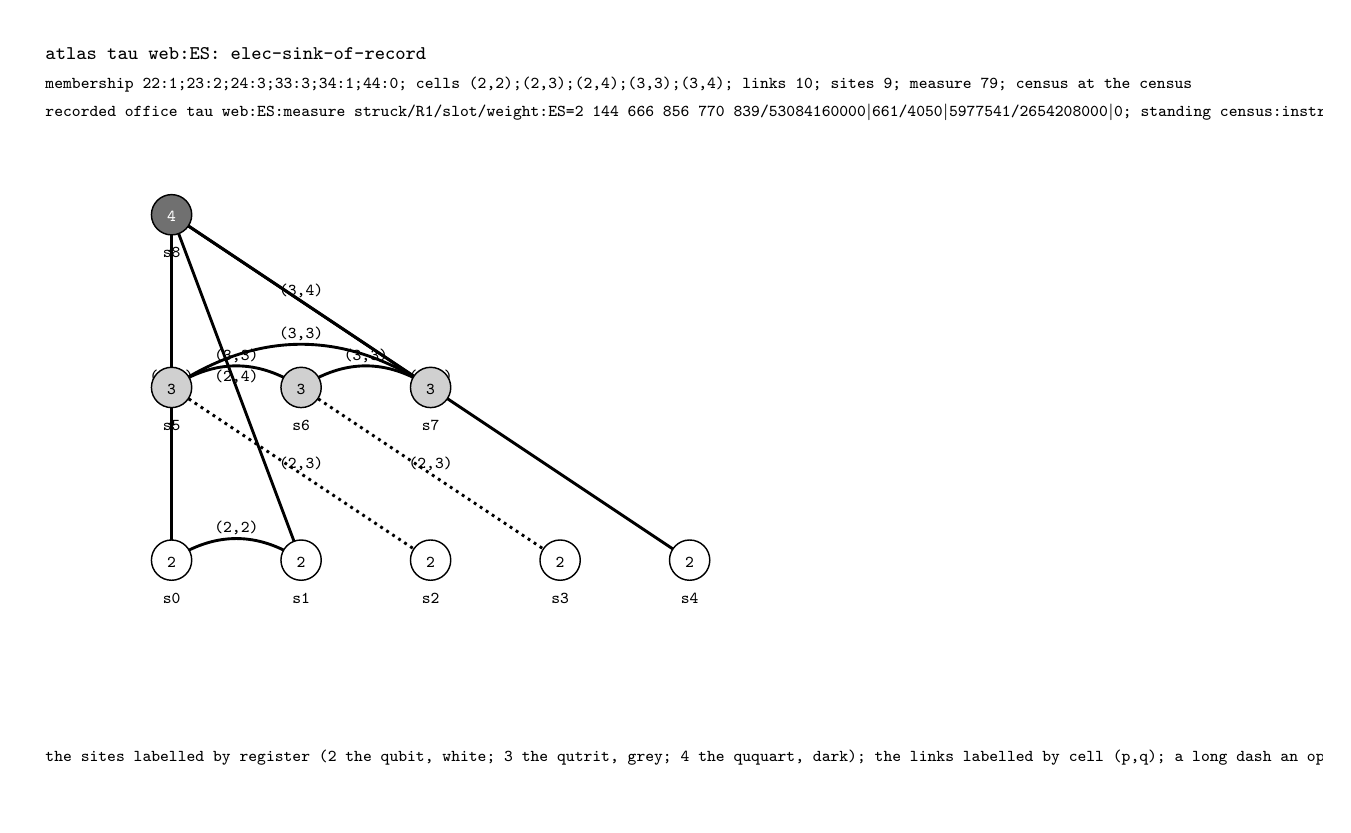
\begin{tikzpicture}[x=0.52pt,y=-0.52pt,baseline]
\clip (0,0) rectangle (900,540);
\fill[white] (0,0) rectangle (900,540);
\node[anchor=base west,inner sep=0pt,text=black,font=\fontsize{6.76}{8.112}\selectfont\ttfamily] at (12,22) {atlas tau web:ES: elec-sink-of-record};
\node[anchor=base west,inner sep=0pt,text=black,font=\fontsize{6.24}{7.488}\selectfont\ttfamily] at (12,42) {membership 22:1;23:2;24:3;33:3;34:1;44:0; cells (2,2);(2,3);(2,4);(3,3);(3,4); links 10; sites 9; measure 79; census at the census};
\node[anchor=base west,inner sep=0pt,text=black,font=\fontsize{5.72}{6.864}\selectfont\ttfamily] at (12,62) {recorded office tau web:ES:measure struck/R1/slot/weight:ES=2 144 666 856 770 839/53084160000\textbar{}661/4050\textbar{}5977541/2654208000\textbar{}0; standing census:instrument;formula:open result;tau web:theorem; board none};
\draw[draw=black,line width=1.04pt] (100,370) .. controls (130,350) and (160,350) .. (190,370);
\node[anchor=base,inner sep=0pt,text=black,font=\fontsize{5.72}{6.864}\selectfont\ttfamily] at (145,351) {(2,2)};
\draw[draw=black,line width=1.04pt] (100,370) -- (100,130);
\node[anchor=base,inner sep=0pt,text=black,font=\fontsize{5.72}{6.864}\selectfont\ttfamily] at (100,246) {(2,4)};
\draw[draw=black,line width=1.04pt] (190,370) -- (100,130);
\node[anchor=base,inner sep=0pt,text=black,font=\fontsize{5.72}{6.864}\selectfont\ttfamily] at (145,246) {(2,4)};
\draw[draw=black,line width=1.04pt,dash pattern=on 1.04pt off 1.56pt] (280,370) -- (100,250);
\node[anchor=base,inner sep=0pt,text=black,font=\fontsize{5.72}{6.864}\selectfont\ttfamily] at (190,306) {(2,3)};
\draw[draw=black,line width=1.04pt,dash pattern=on 1.04pt off 1.56pt] (370,370) -- (190,250);
\node[anchor=base,inner sep=0pt,text=black,font=\fontsize{5.72}{6.864}\selectfont\ttfamily] at (280,306) {(2,3)};
\draw[draw=black,line width=1.04pt] (460,370) -- (100,130);
\node[anchor=base,inner sep=0pt,text=black,font=\fontsize{5.72}{6.864}\selectfont\ttfamily] at (280,246) {(2,4)};
\draw[draw=black,line width=1.04pt] (100,250) .. controls (130,230) and (160,230) .. (190,250);
\node[anchor=base,inner sep=0pt,text=black,font=\fontsize{5.72}{6.864}\selectfont\ttfamily] at (145,231) {(3,3)};
\draw[draw=black,line width=1.04pt] (100,250) .. controls (160,210) and (220,210) .. (280,250);
\node[anchor=base,inner sep=0pt,text=black,font=\fontsize{5.72}{6.864}\selectfont\ttfamily] at (190,216) {(3,3)};
\draw[draw=black,line width=1.04pt] (190,250) .. controls (220,230) and (250,230) .. (280,250);
\node[anchor=base,inner sep=0pt,text=black,font=\fontsize{5.72}{6.864}\selectfont\ttfamily] at (235,231) {(3,3)};
\draw[draw=black,line width=1.04pt] (280,250) -- (100,130);
\node[anchor=base,inner sep=0pt,text=black,font=\fontsize{5.72}{6.864}\selectfont\ttfamily] at (190,186) {(3,4)};
\filldraw[fill=white,draw=black,line width=0.52pt] (100,370) circle (14);
\node[anchor=base,inner sep=0pt,text=black,font=\fontsize{6.24}{7.488}\selectfont\ttfamily] at (100,375) {2};
\node[anchor=base,inner sep=0pt,text=black,font=\fontsize{5.72}{6.864}\selectfont\ttfamily] at (100,400) {s0};
\filldraw[fill=white,draw=black,line width=0.52pt] (190,370) circle (14);
\node[anchor=base,inner sep=0pt,text=black,font=\fontsize{6.24}{7.488}\selectfont\ttfamily] at (190,375) {2};
\node[anchor=base,inner sep=0pt,text=black,font=\fontsize{5.72}{6.864}\selectfont\ttfamily] at (190,400) {s1};
\filldraw[fill=white,draw=black,line width=0.52pt] (280,370) circle (14);
\node[anchor=base,inner sep=0pt,text=black,font=\fontsize{6.24}{7.488}\selectfont\ttfamily] at (280,375) {2};
\node[anchor=base,inner sep=0pt,text=black,font=\fontsize{5.72}{6.864}\selectfont\ttfamily] at (280,400) {s2};
\filldraw[fill=white,draw=black,line width=0.52pt] (370,370) circle (14);
\node[anchor=base,inner sep=0pt,text=black,font=\fontsize{6.24}{7.488}\selectfont\ttfamily] at (370,375) {2};
\node[anchor=base,inner sep=0pt,text=black,font=\fontsize{5.72}{6.864}\selectfont\ttfamily] at (370,400) {s3};
\filldraw[fill=white,draw=black,line width=0.52pt] (460,370) circle (14);
\node[anchor=base,inner sep=0pt,text=black,font=\fontsize{6.24}{7.488}\selectfont\ttfamily] at (460,375) {2};
\node[anchor=base,inner sep=0pt,text=black,font=\fontsize{5.72}{6.864}\selectfont\ttfamily] at (460,400) {s4};
\filldraw[fill={rgb,255:red,208;green,208;blue,208},draw=black,line width=0.52pt] (100,250) circle (14);
\node[anchor=base,inner sep=0pt,text=black,font=\fontsize{6.24}{7.488}\selectfont\ttfamily] at (100,255) {3};
\node[anchor=base,inner sep=0pt,text=black,font=\fontsize{5.72}{6.864}\selectfont\ttfamily] at (100,280) {s5};
\filldraw[fill={rgb,255:red,208;green,208;blue,208},draw=black,line width=0.52pt] (190,250) circle (14);
\node[anchor=base,inner sep=0pt,text=black,font=\fontsize{6.24}{7.488}\selectfont\ttfamily] at (190,255) {3};
\node[anchor=base,inner sep=0pt,text=black,font=\fontsize{5.72}{6.864}\selectfont\ttfamily] at (190,280) {s6};
\filldraw[fill={rgb,255:red,208;green,208;blue,208},draw=black,line width=0.52pt] (280,250) circle (14);
\node[anchor=base,inner sep=0pt,text=black,font=\fontsize{6.24}{7.488}\selectfont\ttfamily] at (280,255) {3};
\node[anchor=base,inner sep=0pt,text=black,font=\fontsize{5.72}{6.864}\selectfont\ttfamily] at (280,280) {s7};
\filldraw[fill={rgb,255:red,112;green,112;blue,112},draw=black,line width=0.52pt] (100,130) circle (14);
\node[anchor=base,inner sep=0pt,text=white,font=\fontsize{6.24}{7.488}\selectfont\ttfamily] at (100,135) {4};
\node[anchor=base,inner sep=0pt,text=black,font=\fontsize{5.72}{6.864}\selectfont\ttfamily] at (100,160) {s8};
\node[anchor=base west,inner sep=0pt,text=black,font=\fontsize{5.72}{6.864}\selectfont\ttfamily] at (12,510) {the sites labelled by register (2 the qubit, white; 3 the qutrit, grey; 4 the ququart, dark); the links labelled by cell (p,q); a long dash an open dark link of the neutron row; a short dash a docked link at the rule R1};
\end{tikzpicture}\end{adjustbox}
\caption{\texttt{elec-sink-of-record}, recorded sink: 9 sites, 10 links, the measure 79; the links at the cells (2,2), (2,3), (2,4), (3,3), (3,4); the membership 22:1; 23:2; 24:3; 33:3; 34:1; 44:0; 2 docked links at the rule R1 (s2-s5; s3-s6); at the census of the six cells. Drawn at the anatomy atlas as its web, the sites labeled by register and the links by cell, from the the roster tau web and the recorded tau sink at the dock rule.}\label{fig:I-5-D540483-elec-sink-of-record-58a580}
\begin{center}\footnotesize\begin{adjustbox}{max width=\linewidth}\begin{tabular}{p{0.26\textwidth}p{0.68\textwidth}}\toprule
recorded office (the slot-count row) & the read o-es of the formula row: the first power 201; the office \texttt{2 144 666 856 770 839/53084160000\textbar{}661/4050\textbar{}5977541/2654208000\textbar{}0}; against the formula with the slot count equal; the slot total 0; dark links 8; hubs s8; dressing 3 \\
mass register (the mass-register row) & the read tes: the class touching the ququart; the first power 201; the office \texttt{2 144 666 856 770 839/53084160000\textbar{}661/4050\textbar{}5977541/2654208000\textbar{}0}; nonzero; met yes; hubs s8; in-legs s7-s8; dressing 3; ports s2-s5; s3-s6; s4-s8 \\
lepton-form office (the lepton row) & the read k-es: the first power 201; the office \texttt{2 144 666 856 770 839/53084160000\textbar{}661/4050\textbar{}5977541/2654208000\textbar{}0}; against the cell equal; dark links 8 \\
\bottomrule\end{tabular}\end{adjustbox}\end{center}
\end{figure}
\begin{figure}[H]\centering
\begin{adjustbox}{max width=\linewidth}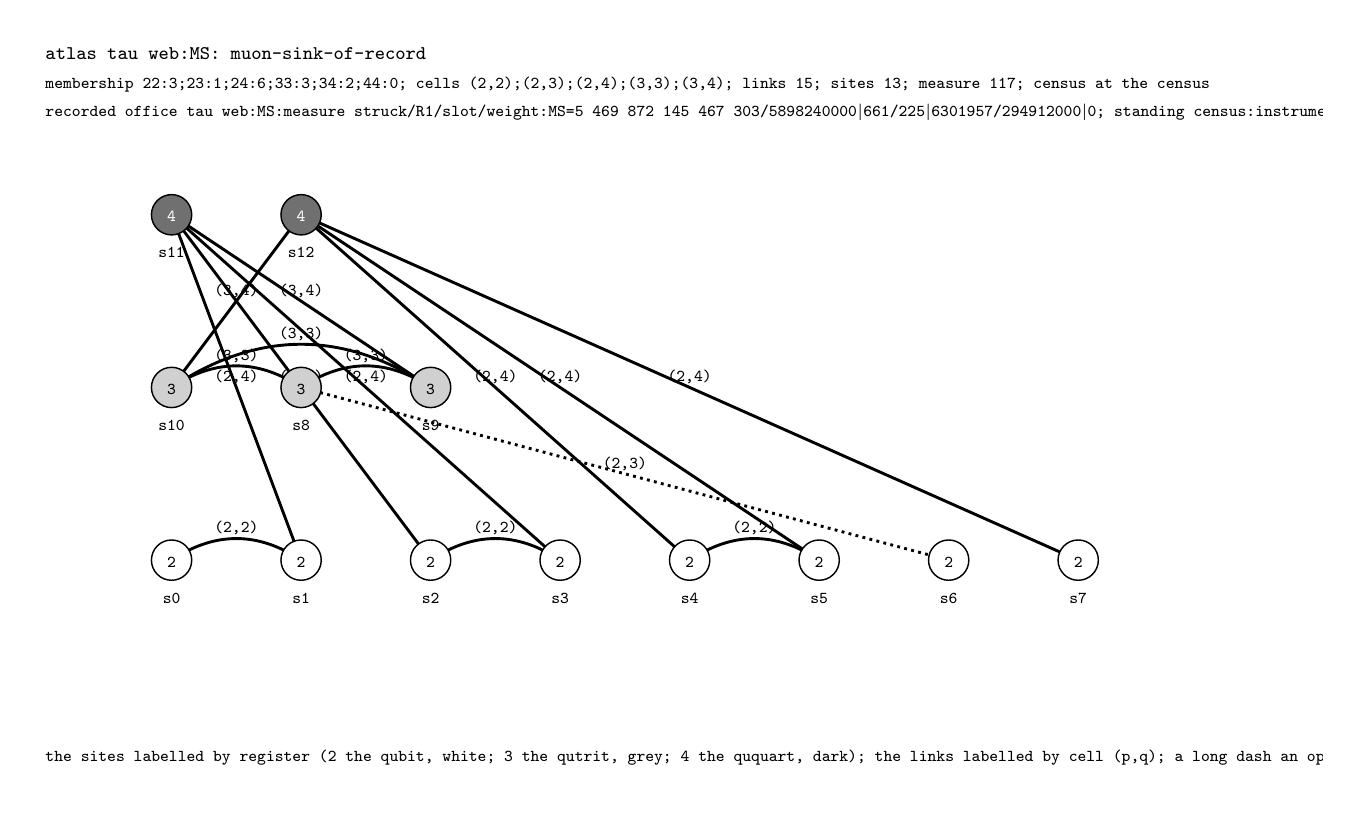
\begin{tikzpicture}[x=0.52pt,y=-0.52pt,baseline]
\clip (0,0) rectangle (900,540);
\fill[white] (0,0) rectangle (900,540);
\node[anchor=base west,inner sep=0pt,text=black,font=\fontsize{6.76}{8.112}\selectfont\ttfamily] at (12,22) {atlas tau web:MS: muon-sink-of-record};
\node[anchor=base west,inner sep=0pt,text=black,font=\fontsize{6.24}{7.488}\selectfont\ttfamily] at (12,42) {membership 22:3;23:1;24:6;33:3;34:2;44:0; cells (2,2);(2,3);(2,4);(3,3);(3,4); links 15; sites 13; measure 117; census at the census};
\node[anchor=base west,inner sep=0pt,text=black,font=\fontsize{5.72}{6.864}\selectfont\ttfamily] at (12,62) {recorded office tau web:MS:measure struck/R1/slot/weight:MS=5 469 872 145 467 303/5898240000\textbar{}661/225\textbar{}6301957/294912000\textbar{}0; standing census:instrument;formula:open result;tau web:theorem; board none};
\draw[draw=black,line width=1.04pt] (100,370) .. controls (130,350) and (160,350) .. (190,370);
\node[anchor=base,inner sep=0pt,text=black,font=\fontsize{5.72}{6.864}\selectfont\ttfamily] at (145,351) {(2,2)};
\draw[draw=black,line width=1.04pt] (190,370) -- (100,130);
\node[anchor=base,inner sep=0pt,text=black,font=\fontsize{5.72}{6.864}\selectfont\ttfamily] at (145,246) {(2,4)};
\draw[draw=black,line width=1.04pt] (100,250) -- (190,130);
\node[anchor=base,inner sep=0pt,text=black,font=\fontsize{5.72}{6.864}\selectfont\ttfamily] at (145,186) {(3,4)};
\draw[draw=black,line width=1.04pt] (100,250) .. controls (130,230) and (160,230) .. (190,250);
\node[anchor=base,inner sep=0pt,text=black,font=\fontsize{5.72}{6.864}\selectfont\ttfamily] at (145,231) {(3,3)};
\draw[draw=black,line width=1.04pt] (100,250) .. controls (160,210) and (220,210) .. (280,250);
\node[anchor=base,inner sep=0pt,text=black,font=\fontsize{5.72}{6.864}\selectfont\ttfamily] at (190,216) {(3,3)};
\draw[draw=black,line width=1.04pt] (100,130) -- (280,370);
\node[anchor=base,inner sep=0pt,text=black,font=\fontsize{5.72}{6.864}\selectfont\ttfamily] at (190,246) {(2,4)};
\draw[draw=black,line width=1.04pt] (100,130) -- (370,370);
\node[anchor=base,inner sep=0pt,text=black,font=\fontsize{5.72}{6.864}\selectfont\ttfamily] at (235,246) {(2,4)};
\draw[draw=black,line width=1.04pt] (100,130) -- (280,250);
\node[anchor=base,inner sep=0pt,text=black,font=\fontsize{5.72}{6.864}\selectfont\ttfamily] at (190,186) {(3,4)};
\draw[draw=black,line width=1.04pt] (190,130) -- (460,370);
\node[anchor=base,inner sep=0pt,text=black,font=\fontsize{5.72}{6.864}\selectfont\ttfamily] at (325,246) {(2,4)};
\draw[draw=black,line width=1.04pt] (190,130) -- (550,370);
\node[anchor=base,inner sep=0pt,text=black,font=\fontsize{5.72}{6.864}\selectfont\ttfamily] at (370,246) {(2,4)};
\draw[draw=black,line width=1.04pt] (190,130) -- (730,370);
\node[anchor=base,inner sep=0pt,text=black,font=\fontsize{5.72}{6.864}\selectfont\ttfamily] at (460,246) {(2,4)};
\draw[draw=black,line width=1.04pt] (280,370) .. controls (310,350) and (340,350) .. (370,370);
\node[anchor=base,inner sep=0pt,text=black,font=\fontsize{5.72}{6.864}\selectfont\ttfamily] at (325,351) {(2,2)};
\draw[draw=black,line width=1.04pt] (460,370) .. controls (490,350) and (520,350) .. (550,370);
\node[anchor=base,inner sep=0pt,text=black,font=\fontsize{5.72}{6.864}\selectfont\ttfamily] at (505,351) {(2,2)};
\draw[draw=black,line width=1.04pt,dash pattern=on 1.04pt off 1.56pt] (640,370) -- (190,250);
\node[anchor=base,inner sep=0pt,text=black,font=\fontsize{5.72}{6.864}\selectfont\ttfamily] at (415,306) {(2,3)};
\draw[draw=black,line width=1.04pt] (190,250) .. controls (220,230) and (250,230) .. (280,250);
\node[anchor=base,inner sep=0pt,text=black,font=\fontsize{5.72}{6.864}\selectfont\ttfamily] at (235,231) {(3,3)};
\filldraw[fill=white,draw=black,line width=0.52pt] (100,370) circle (14);
\node[anchor=base,inner sep=0pt,text=black,font=\fontsize{6.24}{7.488}\selectfont\ttfamily] at (100,375) {2};
\node[anchor=base,inner sep=0pt,text=black,font=\fontsize{5.72}{6.864}\selectfont\ttfamily] at (100,400) {s0};
\filldraw[fill=white,draw=black,line width=0.52pt] (190,370) circle (14);
\node[anchor=base,inner sep=0pt,text=black,font=\fontsize{6.24}{7.488}\selectfont\ttfamily] at (190,375) {2};
\node[anchor=base,inner sep=0pt,text=black,font=\fontsize{5.72}{6.864}\selectfont\ttfamily] at (190,400) {s1};
\filldraw[fill={rgb,255:red,208;green,208;blue,208},draw=black,line width=0.52pt] (100,250) circle (14);
\node[anchor=base,inner sep=0pt,text=black,font=\fontsize{6.24}{7.488}\selectfont\ttfamily] at (100,255) {3};
\node[anchor=base,inner sep=0pt,text=black,font=\fontsize{5.72}{6.864}\selectfont\ttfamily] at (100,280) {s10};
\filldraw[fill={rgb,255:red,112;green,112;blue,112},draw=black,line width=0.52pt] (100,130) circle (14);
\node[anchor=base,inner sep=0pt,text=white,font=\fontsize{6.24}{7.488}\selectfont\ttfamily] at (100,135) {4};
\node[anchor=base,inner sep=0pt,text=black,font=\fontsize{5.72}{6.864}\selectfont\ttfamily] at (100,160) {s11};
\filldraw[fill={rgb,255:red,112;green,112;blue,112},draw=black,line width=0.52pt] (190,130) circle (14);
\node[anchor=base,inner sep=0pt,text=white,font=\fontsize{6.24}{7.488}\selectfont\ttfamily] at (190,135) {4};
\node[anchor=base,inner sep=0pt,text=black,font=\fontsize{5.72}{6.864}\selectfont\ttfamily] at (190,160) {s12};
\filldraw[fill=white,draw=black,line width=0.52pt] (280,370) circle (14);
\node[anchor=base,inner sep=0pt,text=black,font=\fontsize{6.24}{7.488}\selectfont\ttfamily] at (280,375) {2};
\node[anchor=base,inner sep=0pt,text=black,font=\fontsize{5.72}{6.864}\selectfont\ttfamily] at (280,400) {s2};
\filldraw[fill=white,draw=black,line width=0.52pt] (370,370) circle (14);
\node[anchor=base,inner sep=0pt,text=black,font=\fontsize{6.24}{7.488}\selectfont\ttfamily] at (370,375) {2};
\node[anchor=base,inner sep=0pt,text=black,font=\fontsize{5.72}{6.864}\selectfont\ttfamily] at (370,400) {s3};
\filldraw[fill=white,draw=black,line width=0.52pt] (460,370) circle (14);
\node[anchor=base,inner sep=0pt,text=black,font=\fontsize{6.24}{7.488}\selectfont\ttfamily] at (460,375) {2};
\node[anchor=base,inner sep=0pt,text=black,font=\fontsize{5.72}{6.864}\selectfont\ttfamily] at (460,400) {s4};
\filldraw[fill=white,draw=black,line width=0.52pt] (550,370) circle (14);
\node[anchor=base,inner sep=0pt,text=black,font=\fontsize{6.24}{7.488}\selectfont\ttfamily] at (550,375) {2};
\node[anchor=base,inner sep=0pt,text=black,font=\fontsize{5.72}{6.864}\selectfont\ttfamily] at (550,400) {s5};
\filldraw[fill=white,draw=black,line width=0.52pt] (640,370) circle (14);
\node[anchor=base,inner sep=0pt,text=black,font=\fontsize{6.24}{7.488}\selectfont\ttfamily] at (640,375) {2};
\node[anchor=base,inner sep=0pt,text=black,font=\fontsize{5.72}{6.864}\selectfont\ttfamily] at (640,400) {s6};
\filldraw[fill=white,draw=black,line width=0.52pt] (730,370) circle (14);
\node[anchor=base,inner sep=0pt,text=black,font=\fontsize{6.24}{7.488}\selectfont\ttfamily] at (730,375) {2};
\node[anchor=base,inner sep=0pt,text=black,font=\fontsize{5.72}{6.864}\selectfont\ttfamily] at (730,400) {s7};
\filldraw[fill={rgb,255:red,208;green,208;blue,208},draw=black,line width=0.52pt] (190,250) circle (14);
\node[anchor=base,inner sep=0pt,text=black,font=\fontsize{6.24}{7.488}\selectfont\ttfamily] at (190,255) {3};
\node[anchor=base,inner sep=0pt,text=black,font=\fontsize{5.72}{6.864}\selectfont\ttfamily] at (190,280) {s8};
\filldraw[fill={rgb,255:red,208;green,208;blue,208},draw=black,line width=0.52pt] (280,250) circle (14);
\node[anchor=base,inner sep=0pt,text=black,font=\fontsize{6.24}{7.488}\selectfont\ttfamily] at (280,255) {3};
\node[anchor=base,inner sep=0pt,text=black,font=\fontsize{5.72}{6.864}\selectfont\ttfamily] at (280,280) {s9};
\node[anchor=base west,inner sep=0pt,text=black,font=\fontsize{5.72}{6.864}\selectfont\ttfamily] at (12,510) {the sites labelled by register (2 the qubit, white; 3 the qutrit, grey; 4 the ququart, dark); the links labelled by cell (p,q); a long dash an open dark link of the neutron row; a short dash a docked link at the rule R1};
\end{tikzpicture}\end{adjustbox}
\caption{\texttt{muon-sink-of-record}, recorded sink: 13 sites, 15 links, the measure 117; the links at the cells (2,2), (2,3), (2,4), (3,3), (3,4); the membership 22:3; 23:1; 24:6; 33:3; 34:2; 44:0; 1 docked links at the rule R1 (s6-s8); at the census of the six cells. Drawn at the anatomy atlas as its web, the sites labeled by register and the links by cell, from the the roster tau web and the recorded tau sink at the dock rule.}\label{fig:I-5-D540483-muon-sink-of-record-564d76}
\begin{center}\footnotesize\begin{adjustbox}{max width=\linewidth}\begin{tabular}{p{0.26\textwidth}p{0.68\textwidth}}\toprule
recorded office (the slot-count row) & the read o-ms of the formula row: the first power 963; the office \texttt{5 469 872 145 467 303/5898240000\textbar{}661/225\textbar{}6301957/294912000\textbar{}0}; against the formula with the slot count equal; the slot total 0; dark links 14; hubs s11; s12; dressing 9 \\
mass register (the mass-register row) & the read tms: the class touching the ququart; the first power 963; the office \texttt{5 469 872 145 467 303/5898240000\textbar{}661/225\textbar{}6301957/294912000\textbar{}0}; nonzero; met yes; hubs s11; s12; in-legs s9-s11; s10-s12; dressing 9; ports s0-s1; s6-s8; s7-s12 \\
lepton-form office (the lepton row) & the read k-ms: the first power 963; the office \texttt{5 469 872 145 467 303/5898240000\textbar{}661/225\textbar{}6301957/294912000\textbar{}0}; against the cell equal; dark links 14 \\
\bottomrule\end{tabular}\end{adjustbox}\end{center}
\end{figure}
\begin{figure}[H]\centering
\begin{adjustbox}{max width=\linewidth}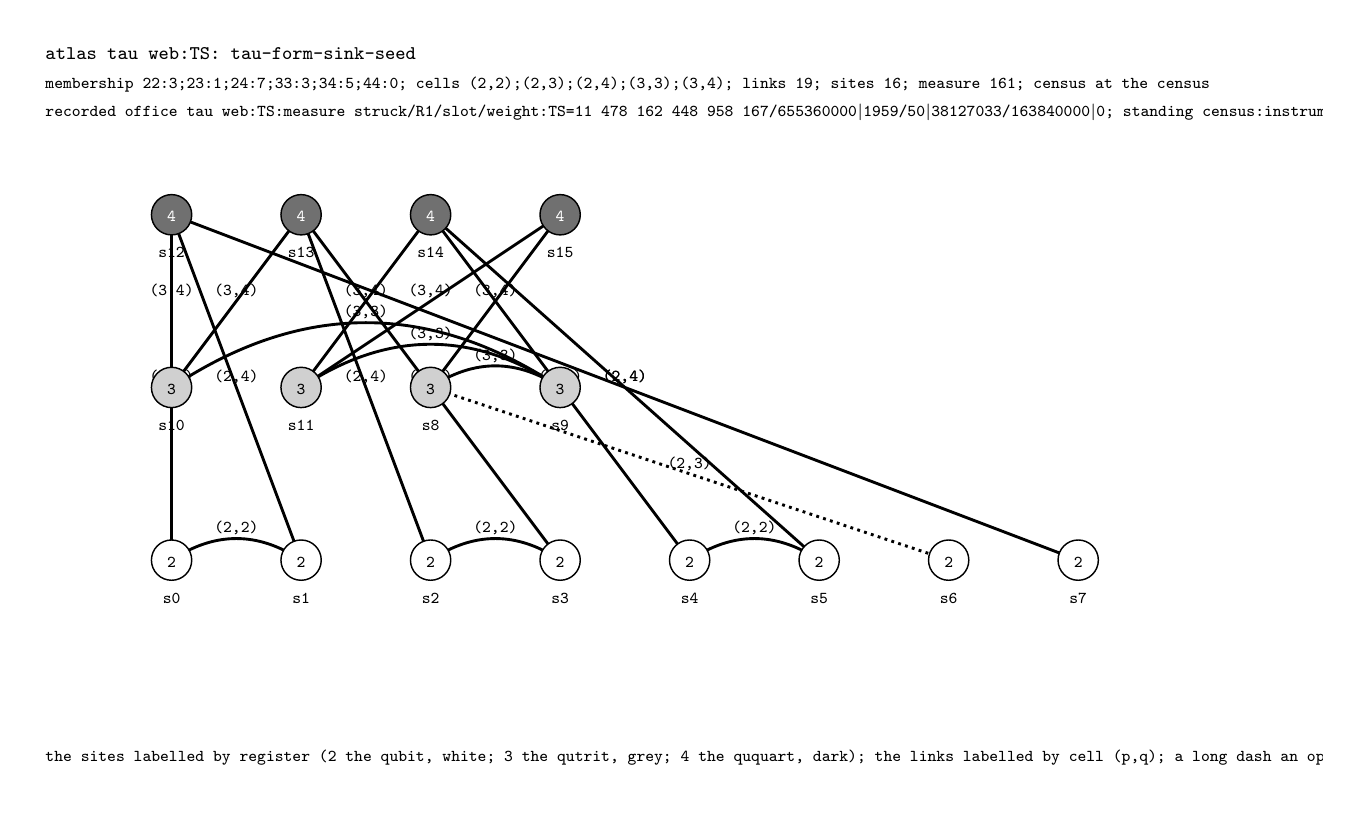
\begin{tikzpicture}[x=0.52pt,y=-0.52pt,baseline]
\clip (0,0) rectangle (900,540);
\fill[white] (0,0) rectangle (900,540);
\node[anchor=base west,inner sep=0pt,text=black,font=\fontsize{6.76}{8.112}\selectfont\ttfamily] at (12,22) {atlas tau web:TS: tau-form-sink-seed};
\node[anchor=base west,inner sep=0pt,text=black,font=\fontsize{6.24}{7.488}\selectfont\ttfamily] at (12,42) {membership 22:3;23:1;24:7;33:3;34:5;44:0; cells (2,2);(2,3);(2,4);(3,3);(3,4); links 19; sites 16; measure 161; census at the census};
\node[anchor=base west,inner sep=0pt,text=black,font=\fontsize{5.72}{6.864}\selectfont\ttfamily] at (12,62) {recorded office tau web:TS:measure struck/R1/slot/weight:TS=11 478 162 448 958 167/655360000\textbar{}1959/50\textbar{}38127033/163840000\textbar{}0; standing census:instrument;formula:open result;tau web:theorem; board none};
\draw[draw=black,line width=1.04pt] (100,370) -- (100,130);
\node[anchor=base,inner sep=0pt,text=black,font=\fontsize{5.72}{6.864}\selectfont\ttfamily] at (100,246) {(2,4)};
\draw[draw=black,line width=1.04pt] (100,370) .. controls (130,350) and (160,350) .. (190,370);
\node[anchor=base,inner sep=0pt,text=black,font=\fontsize{5.72}{6.864}\selectfont\ttfamily] at (145,351) {(2,2)};
\draw[draw=black,line width=1.04pt] (190,370) -- (100,130);
\node[anchor=base,inner sep=0pt,text=black,font=\fontsize{5.72}{6.864}\selectfont\ttfamily] at (145,246) {(2,4)};
\draw[draw=black,line width=1.04pt] (100,250) -- (100,130);
\node[anchor=base,inner sep=0pt,text=black,font=\fontsize{5.72}{6.864}\selectfont\ttfamily] at (100,186) {(3,4)};
\draw[draw=black,line width=1.04pt] (100,250) -- (190,130);
\node[anchor=base,inner sep=0pt,text=black,font=\fontsize{5.72}{6.864}\selectfont\ttfamily] at (145,186) {(3,4)};
\draw[draw=black,line width=1.04pt] (100,250) .. controls (190,190) and (280,190) .. (370,250);
\node[anchor=base,inner sep=0pt,text=black,font=\fontsize{5.72}{6.864}\selectfont\ttfamily] at (235,201) {(3,3)};
\draw[draw=black,line width=1.04pt] (190,250) -- (280,130);
\node[anchor=base,inner sep=0pt,text=black,font=\fontsize{5.72}{6.864}\selectfont\ttfamily] at (235,186) {(3,4)};
\draw[draw=black,line width=1.04pt] (190,250) -- (370,130);
\node[anchor=base,inner sep=0pt,text=black,font=\fontsize{5.72}{6.864}\selectfont\ttfamily] at (280,186) {(3,4)};
\draw[draw=black,line width=1.04pt] (190,250) .. controls (250,210) and (310,210) .. (370,250);
\node[anchor=base,inner sep=0pt,text=black,font=\fontsize{5.72}{6.864}\selectfont\ttfamily] at (280,216) {(3,3)};
\draw[draw=black,line width=1.04pt] (100,130) -- (730,370);
\node[anchor=base,inner sep=0pt,text=black,font=\fontsize{5.72}{6.864}\selectfont\ttfamily] at (415,246) {(2,4)};
\draw[draw=black,line width=1.04pt] (190,130) -- (280,370);
\node[anchor=base,inner sep=0pt,text=black,font=\fontsize{5.72}{6.864}\selectfont\ttfamily] at (235,246) {(2,4)};
\draw[draw=black,line width=1.04pt] (190,130) -- (370,370);
\node[anchor=base,inner sep=0pt,text=black,font=\fontsize{5.72}{6.864}\selectfont\ttfamily] at (280,246) {(2,4)};
\draw[draw=black,line width=1.04pt] (280,130) -- (460,370);
\node[anchor=base,inner sep=0pt,text=black,font=\fontsize{5.72}{6.864}\selectfont\ttfamily] at (370,246) {(2,4)};
\draw[draw=black,line width=1.04pt] (280,130) -- (550,370);
\node[anchor=base,inner sep=0pt,text=black,font=\fontsize{5.72}{6.864}\selectfont\ttfamily] at (415,246) {(2,4)};
\draw[draw=black,line width=1.04pt] (370,130) -- (280,250);
\node[anchor=base,inner sep=0pt,text=black,font=\fontsize{5.72}{6.864}\selectfont\ttfamily] at (325,186) {(3,4)};
\draw[draw=black,line width=1.04pt] (280,370) .. controls (310,350) and (340,350) .. (370,370);
\node[anchor=base,inner sep=0pt,text=black,font=\fontsize{5.72}{6.864}\selectfont\ttfamily] at (325,351) {(2,2)};
\draw[draw=black,line width=1.04pt] (460,370) .. controls (490,350) and (520,350) .. (550,370);
\node[anchor=base,inner sep=0pt,text=black,font=\fontsize{5.72}{6.864}\selectfont\ttfamily] at (505,351) {(2,2)};
\draw[draw=black,line width=1.04pt,dash pattern=on 1.04pt off 1.56pt] (640,370) -- (280,250);
\node[anchor=base,inner sep=0pt,text=black,font=\fontsize{5.72}{6.864}\selectfont\ttfamily] at (460,306) {(2,3)};
\draw[draw=black,line width=1.04pt] (280,250) .. controls (310,230) and (340,230) .. (370,250);
\node[anchor=base,inner sep=0pt,text=black,font=\fontsize{5.72}{6.864}\selectfont\ttfamily] at (325,231) {(3,3)};
\filldraw[fill=white,draw=black,line width=0.52pt] (100,370) circle (14);
\node[anchor=base,inner sep=0pt,text=black,font=\fontsize{6.24}{7.488}\selectfont\ttfamily] at (100,375) {2};
\node[anchor=base,inner sep=0pt,text=black,font=\fontsize{5.72}{6.864}\selectfont\ttfamily] at (100,400) {s0};
\filldraw[fill=white,draw=black,line width=0.52pt] (190,370) circle (14);
\node[anchor=base,inner sep=0pt,text=black,font=\fontsize{6.24}{7.488}\selectfont\ttfamily] at (190,375) {2};
\node[anchor=base,inner sep=0pt,text=black,font=\fontsize{5.72}{6.864}\selectfont\ttfamily] at (190,400) {s1};
\filldraw[fill={rgb,255:red,208;green,208;blue,208},draw=black,line width=0.52pt] (100,250) circle (14);
\node[anchor=base,inner sep=0pt,text=black,font=\fontsize{6.24}{7.488}\selectfont\ttfamily] at (100,255) {3};
\node[anchor=base,inner sep=0pt,text=black,font=\fontsize{5.72}{6.864}\selectfont\ttfamily] at (100,280) {s10};
\filldraw[fill={rgb,255:red,208;green,208;blue,208},draw=black,line width=0.52pt] (190,250) circle (14);
\node[anchor=base,inner sep=0pt,text=black,font=\fontsize{6.24}{7.488}\selectfont\ttfamily] at (190,255) {3};
\node[anchor=base,inner sep=0pt,text=black,font=\fontsize{5.72}{6.864}\selectfont\ttfamily] at (190,280) {s11};
\filldraw[fill={rgb,255:red,112;green,112;blue,112},draw=black,line width=0.52pt] (100,130) circle (14);
\node[anchor=base,inner sep=0pt,text=white,font=\fontsize{6.24}{7.488}\selectfont\ttfamily] at (100,135) {4};
\node[anchor=base,inner sep=0pt,text=black,font=\fontsize{5.72}{6.864}\selectfont\ttfamily] at (100,160) {s12};
\filldraw[fill={rgb,255:red,112;green,112;blue,112},draw=black,line width=0.52pt] (190,130) circle (14);
\node[anchor=base,inner sep=0pt,text=white,font=\fontsize{6.24}{7.488}\selectfont\ttfamily] at (190,135) {4};
\node[anchor=base,inner sep=0pt,text=black,font=\fontsize{5.72}{6.864}\selectfont\ttfamily] at (190,160) {s13};
\filldraw[fill={rgb,255:red,112;green,112;blue,112},draw=black,line width=0.52pt] (280,130) circle (14);
\node[anchor=base,inner sep=0pt,text=white,font=\fontsize{6.24}{7.488}\selectfont\ttfamily] at (280,135) {4};
\node[anchor=base,inner sep=0pt,text=black,font=\fontsize{5.72}{6.864}\selectfont\ttfamily] at (280,160) {s14};
\filldraw[fill={rgb,255:red,112;green,112;blue,112},draw=black,line width=0.52pt] (370,130) circle (14);
\node[anchor=base,inner sep=0pt,text=white,font=\fontsize{6.24}{7.488}\selectfont\ttfamily] at (370,135) {4};
\node[anchor=base,inner sep=0pt,text=black,font=\fontsize{5.72}{6.864}\selectfont\ttfamily] at (370,160) {s15};
\filldraw[fill=white,draw=black,line width=0.52pt] (280,370) circle (14);
\node[anchor=base,inner sep=0pt,text=black,font=\fontsize{6.24}{7.488}\selectfont\ttfamily] at (280,375) {2};
\node[anchor=base,inner sep=0pt,text=black,font=\fontsize{5.72}{6.864}\selectfont\ttfamily] at (280,400) {s2};
\filldraw[fill=white,draw=black,line width=0.52pt] (370,370) circle (14);
\node[anchor=base,inner sep=0pt,text=black,font=\fontsize{6.24}{7.488}\selectfont\ttfamily] at (370,375) {2};
\node[anchor=base,inner sep=0pt,text=black,font=\fontsize{5.72}{6.864}\selectfont\ttfamily] at (370,400) {s3};
\filldraw[fill=white,draw=black,line width=0.52pt] (460,370) circle (14);
\node[anchor=base,inner sep=0pt,text=black,font=\fontsize{6.24}{7.488}\selectfont\ttfamily] at (460,375) {2};
\node[anchor=base,inner sep=0pt,text=black,font=\fontsize{5.72}{6.864}\selectfont\ttfamily] at (460,400) {s4};
\filldraw[fill=white,draw=black,line width=0.52pt] (550,370) circle (14);
\node[anchor=base,inner sep=0pt,text=black,font=\fontsize{6.24}{7.488}\selectfont\ttfamily] at (550,375) {2};
\node[anchor=base,inner sep=0pt,text=black,font=\fontsize{5.72}{6.864}\selectfont\ttfamily] at (550,400) {s5};
\filldraw[fill=white,draw=black,line width=0.52pt] (640,370) circle (14);
\node[anchor=base,inner sep=0pt,text=black,font=\fontsize{6.24}{7.488}\selectfont\ttfamily] at (640,375) {2};
\node[anchor=base,inner sep=0pt,text=black,font=\fontsize{5.72}{6.864}\selectfont\ttfamily] at (640,400) {s6};
\filldraw[fill=white,draw=black,line width=0.52pt] (730,370) circle (14);
\node[anchor=base,inner sep=0pt,text=black,font=\fontsize{6.24}{7.488}\selectfont\ttfamily] at (730,375) {2};
\node[anchor=base,inner sep=0pt,text=black,font=\fontsize{5.72}{6.864}\selectfont\ttfamily] at (730,400) {s7};
\filldraw[fill={rgb,255:red,208;green,208;blue,208},draw=black,line width=0.52pt] (280,250) circle (14);
\node[anchor=base,inner sep=0pt,text=black,font=\fontsize{6.24}{7.488}\selectfont\ttfamily] at (280,255) {3};
\node[anchor=base,inner sep=0pt,text=black,font=\fontsize{5.72}{6.864}\selectfont\ttfamily] at (280,280) {s8};
\filldraw[fill={rgb,255:red,208;green,208;blue,208},draw=black,line width=0.52pt] (370,250) circle (14);
\node[anchor=base,inner sep=0pt,text=black,font=\fontsize{6.24}{7.488}\selectfont\ttfamily] at (370,255) {3};
\node[anchor=base,inner sep=0pt,text=black,font=\fontsize{5.72}{6.864}\selectfont\ttfamily] at (370,280) {s9};
\node[anchor=base west,inner sep=0pt,text=black,font=\fontsize{5.72}{6.864}\selectfont\ttfamily] at (12,510) {the sites labelled by register (2 the qubit, white; 3 the qutrit, grey; 4 the ququart, dark); the links labelled by cell (p,q); a long dash an open dark link of the neutron row; a short dash a docked link at the rule R1};
\end{tikzpicture}\end{adjustbox}
\caption{\texttt{tau-form-sink-seed}, recorded sink: 16 sites, 19 links, the measure 161; the links at the cells (2,2), (2,3), (2,4), (3,3), (3,4); the membership 22:3; 23:1; 24:7; 33:3; 34:5; 44:0; 1 docked links at the rule R1 (s6-s8); at the census of the six cells. Drawn at the anatomy atlas as its web, the sites labeled by register and the links by cell, from the the roster tau web and the recorded tau sink at the dock rule.}\label{fig:I-5-D540483-tau-form-sink-seed-e2eb9e}
\begin{center}\footnotesize\begin{adjustbox}{max width=\linewidth}\begin{tabular}{p{0.26\textwidth}p{0.68\textwidth}}\toprule
recorded office (the slot-count row) & the read o-ts of the formula row: the first power 4185; the office \texttt{11 478 162 448 958 167/655360000\textbar{}1959/50\textbar{}38127033/163840000\textbar{}0}; against the formula with the slot count equal; the slot total 2; dark links 18; hubs s12; s13; s14; dressing 27 \\
mass register (the mass-register row) & the read tts: the class touching the ququart; the first power 4185; the office \texttt{11 478 162 448 958 167/655360000\textbar{}1959/50\textbar{}38127033/163840000\textbar{}0}; nonzero; met yes; hubs s12; s13; s14; in-legs s10-s12; s10-s13; s11-s14; dressing 27; ports s6-s8; s7-s12 \\
lepton-form office (the lepton row) & the read k-ts: the first power 4185; the office \texttt{11 478 162 448 958 167/655360000\textbar{}1959/50\textbar{}38127033/163840000\textbar{}0}; against the cell equal; dark links 18 \\
\bottomrule\end{tabular}\end{adjustbox}\end{center}
\end{figure}
Of the sixty-four listed webs fifty-three are their own sinks at wave zero, while eleven stay unstopped within the budget and at the waves beyond.
\end{chwall}
\chstanding{open result}
\chdeps{Definitions 1.1 to 1.6, Theorems 2.1 to 2.3, Open results 2.4 and 2.5, Theorem 2.6, Open results 2.7 and 2.8 and Theorems 2.9 and 2.10, Theorems 9.1 to 9.7 and Open result 9.8 and Open results 241.1 and 241.2, Theorems 241.3 and 241.4 and Open results 241.5 to 241.7}{the theorems of Chapters 1-4 to 1-5, 3-1, 3-6 to 3-7, 5-3 to 5-7, 5-8f, 5-9, 6-1 to 6-7, 6-7a, 6-10, 7-4 to 7-5, 7-8, 7-10, 8-1, 8-2b, 9-4, 9-6, 10-2, 10-5, 12-1, 12-7, 13-4 to 13-5, 14-1, 14-3, 14-5, 15-1, 15-5, 16-2}
\begin{chtheorem}[The termination of seeded saturation]\label{box:I-5-saturation-in-one-figure-seeds-waves-termination-sinks:3}
Every seeded saturation terminates under the valence bound and the site bound, since the moves map the webs of at most $S$ sites into themselves and such webs are finitely many.
\end{chtheorem}
\chstanding{theorem}
\chdeps{Definitions 1.1 to 1.6, Theorems 2.1 to 2.3, Open results 2.4 and 2.5, Theorem 2.6, Open results 2.7 and 2.8 and Theorems 2.9 and 2.10, Theorems 9.1 to 9.7 and Open result 9.8 and Open results 241.1 and 241.2, Theorems 241.3 and 241.4 and Open results 241.5 to 241.7}{the theorems of Chapters 1-4 to 1-5, 3-1, 3-6 to 3-7, 5-3 to 5-7, 5-8f, 5-9, 6-1 to 6-7, 6-7a, 6-10, 7-4 to 7-5, 7-8, 7-10, 8-1, 8-2b, 9-4, 9-6, 10-2, 10-5, 12-1, 12-7, 13-4 to 13-5, 14-1, 14-3, 14-5, 15-1, 15-5, 16-2}
\begin{chwall}[The seeded saturation at the bound respecting seed]\label{box:I-5-saturation-in-one-figure-seeds-waves-termination-sinks:4}
The bound-respecting seed is a sink the closures do not reach within depth three, and the seed of the proton web is no web of the grammar.
\end{chwall}
\chstanding{open result}
\chdeps{Definitions 1.1 to 1.6, Theorems 2.1 to 2.3, Open results 2.4 and 2.5, Theorem 2.6, Open results 2.7 and 2.8 and Theorems 2.9 and 2.10, Theorems 9.1 to 9.7 and Open result 9.8 and Open results 241.1 and 241.2, Theorems 241.3 and 241.4 and Open results 241.5 to 241.7}{the theorems of Chapters 1-4 to 1-5, 3-1, 3-6 to 3-7, 5-3 to 5-7, 5-8f, 5-9, 6-1 to 6-7, 6-7a, 6-10, 7-4 to 7-5, 7-8, 7-10, 8-1, 8-2b, 9-4, 9-6, 10-2, 10-5, 12-1, 12-7, 13-4 to 13-5, 14-1, 14-3, 14-5, 15-1, 15-5, 16-2}
\begin{chwall}[The closure from the pair ket]\label{box:I-5-saturation-in-one-figure-seeds-waves-termination-sinks:5}
The closure of the act from the pair state reaches none of the seven sinks, the missing letter an attach at a washed end, which is not derived from the Axiom through the definition of open; the closure from the six roots with the join across webs reaches no sink either.
\end{chwall}
\chstanding{open result}
\chdeps{Definitions 1.1 to 1.6, Theorems 2.1 to 2.3, Open results 2.4 and 2.5, Theorem 2.6, Open results 2.7 and 2.8 and Theorems 2.9 and 2.10, Theorems 9.1 to 9.7 and Open result 9.8 and Open results 241.1 and 241.2, Theorems 241.3 and 241.4 and Open results 241.5 to 241.7}{the theorems of Chapters 1-4 to 1-5, 3-1, 3-6 to 3-7, 5-3 to 5-7, 5-8f, 5-9, 6-1 to 6-7, 6-7a, 6-10, 7-4 to 7-5, 7-8, 7-10, 8-1, 8-2b, 9-4, 9-6, 10-2, 10-5, 12-1, 12-7, 13-4 to 13-5, 14-1, 14-3, 14-5, 15-1, 15-5, 16-2}
\begin{chwall}[Rung one as the closure wave one]\label{box:I-5-saturation-in-one-figure-seeds-waves-termination-sinks:6}
Rung one is wave one of the closure, yet the order grading of the sum over records is not the wave grading, the path-count correspondence parting at the first root and wave, and the fourteen listed webs the closure names at a first parting are confirmed web by web.
\end{chwall}
\chstanding{open result}
\chdeps{Definitions 1.1 to 1.6, Theorems 2.1 to 2.3, Open results 2.4 and 2.5, Theorem 2.6, Open results 2.7 and 2.8 and Theorems 2.9 and 2.10, Theorems 9.1 to 9.7 and Open result 9.8 and Open results 241.1 and 241.2, Theorems 241.3 and 241.4 and Open results 241.5 to 241.7}{the theorems of Chapters 1-4 to 1-5, 3-1, 3-6 to 3-7, 5-3 to 5-7, 5-8f, 5-9, 6-1 to 6-7, 6-7a, 6-10, 7-4 to 7-5, 7-8, 7-10, 8-1, 8-2b, 9-4, 9-6, 10-2, 10-5, 12-1, 12-7, 13-4 to 13-5, 14-1, 14-3, 14-5, 15-1, 15-5, 16-2}
\begin{chwall}[The prime content of every web of the network list]\label{box:I-5-saturation-in-one-figure-seeds-waves-termination-sinks:7}
The content grading equals the derived counts at thirteen of the sixteen webs of the direct-sum result; the pumped webs of the list are lowered within their fibres by a readable join save the four zero-sum webs; and the list does not close under lowering at depth two.
\end{chwall}
\chstanding{open result}
\chdeps{Definitions 1.1 to 1.6, Theorems 2.1 to 2.3, Open results 2.4 and 2.5, Theorem 2.6, Open results 2.7 and 2.8 and Theorems 2.9 and 2.10, Theorems 9.1 to 9.7 and Open result 9.8 and Open results 241.1 and 241.2, Theorems 241.3 and 241.4 and Open results 241.5 to 241.7}{the theorems of Chapters 1-4 to 1-5, 3-1, 3-6 to 3-7, 5-3 to 5-7, 5-8f, 5-9, 6-1 to 6-7, 6-7a, 6-10, 7-4 to 7-5, 7-8, 7-10, 8-1, 8-2b, 9-4, 9-6, 10-2, 10-5, 12-1, 12-7, 13-4 to 13-5, 14-1, 14-3, 14-5, 15-1, 15-5, 16-2}
\begin{chwall}[The attach-site invariance at the joined webs]\label{box:I-5-saturation-in-one-figure-seeds-waves-termination-sinks:8}
The readout parts across the open sites at every admitted web, first at the listed muon; the type closure holds at all but three seeded saturations, no end of dimension five or seven reached; the sector-to-ends map is not a rule of the moves at the sinks; and the valence bound is broken at the seeded sinks where the seeds carry it.
\end{chwall}
\chstanding{open result}
\chdeps{Definitions 1.1 to 1.6, Theorems 2.1 to 2.3, Open results 2.4 and 2.5, Theorem 2.6, Open results 2.7 and 2.8 and Theorems 2.9 and 2.10, Theorems 9.1 to 9.7 and Open result 9.8 and Open results 241.1 and 241.2, Theorems 241.3 and 241.4 and Open results 241.5 to 241.7}{the theorems of Chapters 1-4 to 1-5, 3-1, 3-6 to 3-7, 5-3 to 5-7, 5-8f, 5-9, 6-1 to 6-7, 6-7a, 6-10, 7-4 to 7-5, 7-8, 7-10, 8-1, 8-2b, 9-4, 9-6, 10-2, 10-5, 12-1, 12-7, 13-4 to 13-5, 14-1, 14-3, 14-5, 15-1, 15-5, 16-2}
\begin{chconditional}[The cut rank at a joined web]\label{box:I-5-saturation-in-one-figure-seeds-waves-termination-sinks:9}
Conditional on the results this theorem rests on at their own standing, as its derivation names them.
The Schmidt rank across every cut of every joined web is the product of the ranks of the crossing pairs, one crossing pair a bond and more a throat; at every two-sided web the cargo record appears at the far body with the chain and nowhere without it, conditional on the light-cone premise; and the electron office at the whole sink is a theorem placed here and read at its grade.
\end{chconditional}
\chstanding{conditional theorem}
\chdeps{Definitions 1.1 to 1.6, Theorems 2.1 to 2.3, Open results 2.4 and 2.5, Theorem 2.6, Open results 2.7 and 2.8 and Theorems 2.9 and 2.10, Theorems 9.1 to 9.7 and Open result 9.8 and Open results 241.1 and 241.2, Theorems 241.3 and 241.4 and Open results 241.5 to 241.7}{the theorems of Chapters 1-4 to 1-5, 3-1, 3-6 to 3-7, 5-3 to 5-7, 5-8f, 5-9, 6-1 to 6-7, 6-7a, 6-10, 7-4 to 7-5, 7-8, 7-10, 8-1, 8-2b, 9-4, 9-6, 10-2, 10-5, 12-1, 12-7, 13-4 to 13-5, 14-1, 14-3, 14-5, 15-1, 15-5, 16-2}
The closures are run from their roots under the moves at the bounds of their entries and the reach results of the list re-met web by web. The termination follows from the self-map of the moves and the finite count of labeled webs, the table carrying every move with its inverse. The crossing part of every cut is a product of pair states, its rank the product of the smaller end dimensions, computed exactly by elimination. The two-sided webs are built with and without the chain and the cargo record read at the far body of every one.

\begin{chbridge}
The forward closure of a set under a finite family of operations is its orbit, graded by the layer at which each element is first reached. The derivation supplies the closure of the admitted moves from a seed with its waves and sinks here, and the bodies named the electron, the muon and the proton, the light-cone premise and the ranks named for Schmidt are named by correspondence.
\end{chbridge}
\begin{chproof}[census]
The premises are the axiom with its definition of a web (chapter 1-1, the text), the moves in one table with their inverses (chapter 1-4, a theorem), the valence bound at the sites (a conditional theorem placed at no chapter of this compendium) and the listed webs as seeds (chapter 1-5, an instrument read at its standing). The chain back to the axiom runs through chapter 1-4 and the framework chapter. By exhaustive enumeration of the one hundred thirty-three thousand nine hundred eighty-three applications of the twenty-eight admitted moves at the three web tables of the derivation and of the eight thousand five hundred sixty-three applications at the listed webs (the set generated by every move applied at every web of those tables under the valence bound and the site bound). The property tested at every application being whether the move maps a web of at most $S$ sites with the degree at most the dimension at every site to another such web, the self-map. The counts by kind, the self-map re-met at every application, one hundred thirty-three thousand nine hundred eighty-three of one hundred thirty-three thousand nine hundred eighty-three and eight thousand five hundred sixty-three of eight thousand five hundred sixty-three. The labeled webs of at most $S$ sites counted at most
\begin{equation}
N(S) = \sum_{s=1}^{S} 3^{s}\,(s+1)^{4s} ,
\end{equation}
a sixty-digit integer at $S = 12$ and an eight-hundred-nineteen-digit integer at $S = 97$, so the reachable set from any seed of at most $S$ sites is finite and the pairing-move saturation from it stops at a wave at most $N(S) - 1$, the table carrying every move with its inverse so that no potential rises at every move. At the listed seeds the saturations run at fifty-three and complete at twenty-nine, eighteen stopped at the sink condition and eleven exhausted, every one within the wave bound and the size bound at twenty-nine of twenty-nine with the excess over the dimension grown nowhere, twenty-four at the check bound of twelve sites unstopped at the web cap as an initial segment each, and the thirty-six listed webs beyond twelve sites refused at the site bound. The first parting element none, so every seeded saturation terminates under the valence bound and the site bound, which is the theorem. With the site bound lifted to a demonstration cap of forty the first site-creating move of the table that grows without bound is the cut at the seed of the third root, five to forty-one sites in nine applications at four sites each, and the first join across two webs that grows without bound is the third join at the gluon seed, four to forty sites in nine joins of copies, printed beside. The smallest case on the page is the seed of a single site, the one web of at most one site is counted at $N(1) = 3\cdot 2^{4} = 48$ labeled webs, so a saturation from it stops within forty-seven waves.

The counter-tests struck the site bound, which moved eighty-three cells beginning at the status of a saturation. struck the valence bound, which moved one hundred ninety-six cells beginning at a control, and struck the text at its gate, which moved every cell. Every control read the same at both engines, nine of nine, and the self-map and the bound were reproduced at a second engine built apart, equal at every cell.
\chcert{133983}
\end{chproof}
\section{The sector-to-ends map at the parting web}\label{mod:I-5-D534928-w-smrp}
\begin{chwall}[The sector-to-ends map at the parting web]\label{box:I-5-D534928-w-smrp:1}
No adopted reading named apart closes both partings of the sector-to-ends map at the sinks the admitted moves reach: at the rewrite reading the one move reaching the sink from the listed star target hands the proton dock both ends, so the star clause closes, while the electron pair link reads both ends as well against none, so the electron clause stands; at the spare reading and at the transport reading the electron clause closes while the dock link reads one end at the seed and at the sink, so the star clause stands; at the open-anywhere reading both clauses stand, and at the union reading every link reads both ends, closing the star clause and leaving the electron clause standing. The open result is entered at the letter that the parting stands at every reading.
\end{chwall}
\chstanding{open result}
\chdeps{Definitions 1.1 to 1.6 and Open results 245.1 and 245.2, Theorem 245.3, Open results 245.4 to 245.8 and Theorem 245.9}{no theorem beyond it at this release}
The parting web is named, the sector-to-ends map is assigned at every one of the five adopted readings named apart, the moves reaching the sinks from the seeds are listed with the link entries they transfer, and at every reading the two clauses, the star clause at the proton dock and the electron clause at the pair link, are read at the sinks; no reading closes both, so the record-sector route derives the ladder assignment at no move-defined reading at the sinks.

\begin{chbridge}
In the electroweak theory the left-handed fermions are assigned to doublets of the weak isospin group and the right-handed fermions to singlets, the assignment of each field to its representation a postulate of the model and derived from no dynamics \cite{Glashow1961,Weinberg1967}. The derivation supplies the end sets of the links at the sinks and the moves that transfer them here, and the proton and the electron, with their mass and their binding, are named by correspondence.
\end{chbridge}
\begin{chproof}[finite]
The premises are the moves in one table (chapter 1-4, a theorem), the saturation with its seeds and sinks (chapter 1-5, a theorem) and the sector-to-ends map at the spectrum (chapter 1-5, an open result read at its standing). The chain back to the axiom runs through chapter 1-5 and the framework chapter. The procedure. The input is the parting web, the star target at the proton side and the electron at its own sink, with the fifty-six admitted moves and the five readings of the sector-to-ends map named apart, the rewrite, spare, transport, open-anywhere and union readings. For every reading the map assigns an end set, none, one or both, to every link at the seed and at the sink, and the moves reaching the sinks from the seeds are listed with the link entries they transfer. The test applied at every reading is the pair of clauses, the star clause that the proton dock, a (2,3) link, reads both ends at the sink the moves reach, and the electron clause that the electron pair link, a (2,2) link, reads no end at its sink. The aggregation counts, reading by reading, the clauses that close and the first parting link. The totals at the checkpoints, at the rewrite reading the one move reaching the star sink, the within-web join of the two arms with spare, the twelfth of the fifty-six, transfers the dock link from one end at the seed to both at the sink, every dock of the star sink at both, three of three, so the star clause closes, while the electron pair link reads both ends against none with its links at no end at zero of ten, so the electron clause stands. At the spare and transport readings the electron links read no end at seven of ten and four of ten, so the electron clause closes, while the dock reads one end at the seed and at the sink with the star docks at both at zero of three, so the star clause stands. At the open-anywhere reading both clauses stand. At the union reading every link reads both ends, closing the star clause and leaving the electron clause standing,
\begin{equation}
\text{readings closing both clauses} = 0 \text{ of } 5 ,
\end{equation}
which is the open result, the first parting overall at the rewrite reading at the electron clause, the pair link at both ends against none. The smallest instance on the page is the electron at the rewrite reading, it is its own sink, no move transfers any end at it, and its pair link reads both ends where the ladder asks none.

The counter-tests re-keyed the reading order, which moved the first parting. struck a move, which moved no cell as pinned. struck the closed-link counts at every reading, which moved them. re-keyed the link entries of the star and the electron webs, which moved every transfer cell, and struck the text at its gate, which moved every cell. Every control read the same at both engines, fourteen of fourteen, and the readings were reproduced at a second engine, equal at every cell.
\chcert{56}
\end{chproof}
\section{The Standard Model list at the saturated sinks}\label{mod:I-5-D538426-w-msss}
\begin{chwall}[The Standard Model list at the saturated sinks]\label{box:I-5-D538426-w-msss:1}
At the derived saturated sinks the list of the board, at its names and grade tokens alone, is re-met at two columns: the hub-count column as the second census read it, with four of its six entries derived and the generation labels parting at that material, and the attach-site column with all six entries derived, the three lepton labels present among the attach-site counts of the seven hundred forty-five lepton-form sinks and the four quark labels among those of the quark-form sinks. The two readings part sink by sink: the generation count by the hub count and by the attach-site count agree at one hundred fifty-three of the lepton-form sinks, parting first at a proton sink, and the attach-site basis is a derived structure at twenty of them alone. The open result is entered with both cells named, the base material an initial segment at the budgets of its entries and nothing read as a closure.
\end{chwall}
\chstanding{open result}
\chdeps{Definitions 1.1 to 1.6 and Open results 245.1 and 245.2, Theorem 245.3, Open results 245.4 to 245.8 and Theorem 245.9}{no theorem beyond it at this release}
The list is re-met at the two columns over the sinks of the proton saturation and the tau-sink saturation, the hub-count reading at the wider material reaching the third label with a fourth beside, and the two readings are compared sink by sink with the first parting and the first undefined sink named; the two engines agree at every key and the runs are byte-identical.

\begin{chbridge}
The particle content of the Standard Model is a list: three generations of leptons and quarks, the gauge bosons of the three interactions and the Higgs, each entry at its charges under the gauge group, the list fixed by the representations chosen and read from the spectrum of the bodies found at the colliders \cite{Glashow1961,Weinberg1967}. The derivation supplies the hub counts and the attach-site counts of the sinks here, and the generations named and the lepton and quark labels are named by correspondence, the list standing at chapter 4-10.
\end{chbridge}
\begin{chproof}[census]
The premises are the saturation with its sinks (chapter 1-5, a theorem), the lepton-form sinks of the tau-sink saturation (an open result placed at no chapter of this compendium, read at its standing) and the list of the board at its names and grade tokens (chapter 4-10, an instrument). The chain back to the axiom runs through chapter 1-5 and the framework chapter. By exhaustive enumeration of the sixteen thousand nine hundred sixty-two saturated sinks of the proton saturation and the tau-sink saturation (the set generated by the admitted moves from the seeds to the budgets of those two derivations, an initial segment and nothing read as a closure), among them the seven hundred forty-five lepton-form sinks and the quark-form sinks. The property tested being whether the generation label of a sink read by its hub count and read by its attach-site count agree, and whether the attach-site basis is a derived structure at the sink. The counts by kind, the three lepton labels present among the attach-site counts of the lepton-form sinks at three of three and the four quark labels among those of the quark-form sinks, six of six entries derived at the attach-site column against four of six at the hub-count column of the second census. The two readings equal at one hundred fifty-three of the seven hundred forty-five lepton-form sinks,
\begin{equation}
n_{\text{hub}} = n_{\text{attach}} \ \text{at } 153 \text{ of } 745,\qquad \text{the basis derived at } 20 \text{ of } 745 ,
\end{equation}
the first parting element a proton sink with the hub count two against the attach-site count one, and the first sink at which the basis is undefined a proton sink with no core triangle. So the list is re-met at two columns that part sink by sink, which is the open result. The smallest case on the page is the listed ladder with its electron seeded sink, the attach-site basis is a derived structure there at two of two ladder webs and one of one seeded sink, and the two counts agree.

The counter-tests struck the attach site, which moved thirty-one cells beginning at the first undefined sink. struck a basis vector, which moved forty-one cells beginning at the basis, and struck the text at its gate, which left the gate unmet. Every control read the same at both engines, the two engines equal at every key with the runs byte-identical, and the counts were reproduced at a second engine, equal at every sink.
\chcert{16962}
\end{chproof}
\section{The record rule at the closure from the known clause}\label{mod:I-5-D538628-w-lrkc}
\begin{chwall}[The closure under the record rule and the third clause of known]\label{box:I-5-D538628-w-lrkc:1}
The closure under the record rule is not the closure under the third clause of the definition \emph{known}: the one hundred sixty-nine records of the arrow-resolvent result are pairs of letters at two distinct slots of the alpha star, and the clause that two reads commuting only up to a sign are a further record generates from the twenty-two reads of the star a set of records equal to them at none of the six letter-and-sign readings computed, twenty-six records at the adopted reading, ten among the one hundred sixty-nine and sixteen beyond them; the rule as used at the closure carries four clauses beyond the words of the known clause, and the known clause three beyond the rule, while at the Weyl letters at the strict sign the same-slot records of the clause equal the closure cells at both ends. The open result is entered with both faces named, conditional on the results it rests on.
\end{chwall}
\chstanding{open result}
\chdeps{Definitions 1.1 to 1.6, Theorems 2.1 to 2.3, Open results 2.4 and 2.5, Theorem 2.6, Open results 2.7 and 2.8 and Theorems 2.9 and 2.10 and Open results 245.1 and 245.2, Theorem 245.3, Open results 245.4 to 245.8 and Theorem 245.9}{no theorem beyond it at this release}
The records of the arrow-resolvent result are read as pairs of letters at two slots, the known clause is applied to the twenty-two reads at six readings of letter and sign, the generated records are compared with the admitted records with the first record not generated and the first generated record not admitted both named, the clauses of the rule as used and of the known clause are compared word by word, and the commutator records are recounted at the Weyl letters.

\begin{chbridge}
The observables of a quantum register that commute with every element of a set generate its commutant, and two Pauli-type operators either commute or anticommute, their product a further element of the group up to a sign; the stabilizer formalism reads the state fixed by a commuting set of such operators, and the degree-two elements of a Clifford algebra close under the bracket \cite{Gottesman1997,Weyl1927}. The derivation supplies the Weyl relation and the commutator records on a tensor product here, and any coupling or vertex named through the arrow-resolvent result is named by correspondence.
\end{chbridge}
\begin{chproof}[exact]
The premises are the axiom with the third clause of the definition \emph{known} (chapter 1-1, the text), the record phase group at every type (chapter 1-2, a theorem) and the arrow-resolvent result with its one hundred sixty-nine records (chapter 2-6, a theorem). The chain back to the axiom runs through chapter 1-1 and the framework chapter. From the alpha star, by the enumeration of its slots and their traceless letters, we obtain four slots at the words of the star, the center and the far slot of each of two arms, with eight, three, eight and three letters, and the twenty-two reads,
\begin{equation}
8 + 3 + 8 + 3 = 22 ,
\end{equation}
and from the pairs of letters at two distinct slots, by the count of the pairs block by block, the one hundred sixty-nine records of the arrow-resolvent result,
\begin{equation}
8\cdot 3 + 8\cdot 8 + 8\cdot 3 + 3\cdot 8 + 3\cdot 3 + 8\cdot 3 = 24 + 64 + 24 + 24 + 9 + 24 = 169 .
\end{equation}
From the twenty-two reads, by the third clause of \emph{known} (two reads that commute only up to a sign are a further record, their order the sign) at the reading taken, the Hermitian traceless letters at the strict sign with a record a pair of reads, we obtain twenty-six generated records, ten of them among the one hundred sixty-nine and sixteen beyond them,
\begin{equation}
26 = 10 + 16,\qquad 169 - 10 = 159 \ \text{records of the result the clause does not generate} ,
\end{equation}
the first record of the result not generated being the pair of the first center letter and the first far letter of one arm, two reads at distinct qudits that commute exactly, and the first generated record not admitted being the pair of the first two center letters at one slot. Over the six readings of letter and sign (Hermitian, Weyl or Chevalley letters at the strict or the wide sign) the generated set equals the one hundred sixty-nine at none, the shared counts being ten, one hundred twenty-nine, zero, one hundred twenty-one, eight and one hundred thirty-five. From the words of the rule as used at the closure (a record counted when the bracket on the second exterior power maps it injectively into the end algebra) against the words of the clause, by a comparison clause by clause, we obtain four clauses of the rule beyond the clause, the first the records at an end algebra, and three clauses of the known clause beyond the rule, the words pair, reads, commute, sign, further and order. So the closure under the rule as used is not the closure under the clause, which is the open result, with the first parting at the first admitted record the clause does not generate. The smallest instance on the page is one qubit slot at the Weyl letters at the strict sign, its three letters anticommute pairwise, so the clause generates three same-slot records there, equal to the three commutator records of the closure at that end, while at a qutrit slot the Weyl letters commute up to a cube root and the clause generates none, equal to the zero of the closure. The two rules meet at those counts and part at the words and at the one hundred sixty-nine records.

The counter-tests moved the reading of the letters and of the sign through the six readings, at every one of which the comparison stayed unequal, and struck the text of the clause at its gate. Every control read the same at both engines, among them the Weyl relation at dimension two, the end orders four and twelve of the record phase group and the commutation phases at dimensions two and three. The generated sets and the counts were reproduced at a second engine built on the group ring, equal at every cell.
\end{chproof}
\begin{figure}[h]\centering
\begin{adjustbox}{max width=\linewidth}\begin{tabular}{llrr}\toprule
slot of the star & site & traceless letters & reads \\ \midrule
the center slot of the first arm & a qutrit & 8 & 8 \\
the far slot of the first arm & a qubit & 3 & 3 \\
the center slot of the second arm & a qutrit & 8 & 8 \\
the far slot of the second arm & a qubit & 3 & 3 \\ \midrule
the star & & 22 & 22 \\ \bottomrule
\end{tabular}\end{adjustbox}
\caption{The alpha star at its four slots: the site of each slot, its traceless letters and its reads; a record of the arrow-resolvent result is a pair of letters at two distinct slots, one hundred sixty-nine in all.}
\end{figure}
\section{The move graph at the saturated sinks}\label{mod:I-5-D539442-w-gskm}
The particle table of the Standard Model is read as a directed graph of decays and productions: every unstable state has forward edges to the final states its decays reach, the stable states are the sinks of the graph with no forward edge, and the branching of a decay among its channels is a property of the matrix elements at the vertex and of the phase space of the final state \cite{Griffiths2008,Weinberg1995}. The saturation and its sinks are introduced at section~\ref{mod:I-5-saturation-in-one-figure-seeds-waves-termination-sinks} and decay as the forward edge of a non-sink at section~\ref{mod:IX-1-decay-as-the-forward-edge-of-a-non-sink-the-move-graph-of-the-hub-step}.
The 28 moves of the move table, applied at every site of every one of the 16962 nodes of the sink census, yield 3081272 applications, of which 584612 fall among the three kinds the question names: 68044 reach a census sink, the sink-to-sink edges of the graph; 491484 reach a non-sink, the forward edges of the decay graph; and 25084 give no result, the reverse hub step refused at the in-site; while 2496660 reach a sink the census does not carry.
The graph is built at every node, with 68044 edges, 2153 components and 40278 forward edges, the word is read at every node and the forward edges are printed. The first application reaching a sink outside the census is at the roster web rost-1, at the attachment numbered 23 at its dock s0.n1: the result is a sink of 23 sites and 25 links at measure 194, with two (2,2) links, seven (2,3), six (2,4), eight (3,3) and two (3,4), isomorphic to no node of the census and none beyond the canonical bound. The edge from rost-1 to that sink is an edge the census sinks do not carry; two independent implementations agree at every value and the runs are byte-identical.
The result is an open one, an open result: the stronger statement, that the graph is an output of the census and the move table with every listed value read from it, is not met at the census as it stands, and the weaker statement is named with both values; no comparison with observation is made here.
What stays open is the graph at a census carrying every reached sink; the move graph of the hub step (section~\ref{mod:IX-1-decay-as-the-forward-edge-of-a-non-sink-the-move-graph-of-the-hub-step}) and the decay board beside it have been read together with this graph by no result.
\section{The closure taken whole at the five bodies}\label{mod:I-5-D539571-epcl-t1}
In quantum electrodynamics the self-energy of a charged lepton is the sum of the one-particle-irreducible insertions on its propagator, each insertion a closed loop of the field attached at two vertices; the mass shift is the self-energy at the pole, and the contributions of distinct loops add at a given order with cross terms between loops sharing a vertex \cite{Dyson1949,Peskin1995}. The saturation and its sinks are introduced at section~\ref{mod:I-5-saturation-in-one-figure-seeds-waves-termination-sinks} and the body-alone office rule at section~\ref{mod:VIII-2-body-alone-office-rule}.
At the reading fixed for the office, where the act read of every link is taken from the segment theorem by locator, the dark set is every link of a genre other than (2,3), the single closure at a dark link is the square of its act read multiplied by the weight G2, and a pair closure is kept whole when some pair record survives the wash at the shared end, the electron pair closure is an exact value beside the single closures: the 13 pairs of dark links sharing an end at the electron are every one kept at their shared end, and the pair closure is the positive element 5941216111 over 238878720000 plus 551257 over 29160000 root 2 plus 18028823 over 19906560000 root 3 plus 427 over 1620000 root 6.
The office taken whole is exact at 6 of 6 reads, and the single closures and the offices derived from them are reproduced. The proton is unmoved: its 9 pairs at 5 shared ends are kept by the wash, but every amplitude is zero because every dark link of the proton reads at nothing beyond the first cap, so its pair closure is zero and its office taken whole, 8242641, equals the office from the single closures alone. The muon and the reference tau web carry positive pair closures at their pairs, and the neutron through the deuteron a zero one.
The result is a theorem: the closure taken whole at the five bodies follows from the axiom at the stated reading, conditional on the results it cites at their own standing; no comparison with observation is made here.
What stays open is the reading of this closure together with the body-alone office rule at the mass readout of Part X, which no result has made; a refuting case is found at none.
\section{The saturation resumed at a larger count}\label{mod:I-5-D539599-w-audt}
The hadron spectrum of the quark model is an infinite tower: beyond the lowest multiplets of mesons and baryons every flavour content carries radial and orbital excitations of rising mass, so a roster of states cut at any finite mass is an initial segment of the spectrum and not the spectrum itself, and the states of that segment are joined to the states beyond it by decays and productions \cite{GellMann1964,Griffiths2008}. The saturation and its sinks are introduced at section~\ref{mod:I-5-saturation-in-one-figure-seeds-waves-termination-sinks} and the mesons and the nucleon at the cap at the chapter titled The mesons and the nucleon at the cap (chapter~\ref{mod:VII-9-mesons-and-the-nucleon-at-the-cap}, among the instruments).
The saturation that produced the tau sink is resumed from its chain at the faces seed, electron and star in the order of the roots table, at fourfold the original budget of 90, 360 run pieces per implementation; the sinks found at the original run stand as an initial segment of the resumed run, and the join of the resumed sinks against the standing sinks parts at a named sink.
The initial segment of the original run is reproduced at every compared wave by canonical key at both implementations, each running 226 pieces with none carried and none finished, the budget not exhausted; the three faces stop cut at the bound, seed at wave 4, electron at wave 3 and star at wave 3. The 44642 sinks reached by the join are read at the cross-term theorem by its own functions: 43663 agree and are typed composite, 979 part. Within the webs the lepton-form sinks fall at the hub counts 104, 346, 1217 and 1085 at hubs zero to three with 1652 beyond, so that a fourth within-web label is present beside the three of the ladder; among the join-reached sinks the counts are 53, 215, 505 and 566 with 4509 beyond.
The result is an open one, an open result: the resumed saturation reaches sinks beyond the standing ones and the join parts at a named sink, so the result stands at the weaker reading; no comparison with observation is made here.
What stays open is the census of the saturated sinks (section~\ref{mod:I-5-D538426-w-msss}) read together with the resumed run at a larger count, which no result has done.
\section{The neutron closure at its own typing}\label{mod:I-5-D539893-w-tcln}
\begin{chwall}[The neutron closure at its own typing]\label{box:I-5-D539893-w-tcln:1}
At the count of its own typing through the deuteron, two thousand eight hundred seventy-one, equal to the proton count, the office of the neutron at the body alone by the one rule is the count squared plus a closure over the eight dark links its typing leaves open, and at the act read of the typing, where a link read at nothing closes at nothing, that closure is zero and the office, eight million two hundred forty-two thousand six hundred forty-one, equals the proton office. The first face, the neutron office the count squared plus a positive closure over the open set, the neutron parting from the proton by a closure and not by a count, is unmet at the act read; the second face, the closure zero at the open set, is met, and the first parting is the closure zero at the open set. At the mass-row weight of the count read beside, the closure over the same eight links is the exact positive element $\tfrac{135253}{480000} + \tfrac{8}{75}\sqrt{2} + \tfrac{153413}{30720000}\sqrt{3}$ and the neutron office parts from the proton office by that closure.
\end{chwall}
\chstanding{open result}
\chdeps{Definitions 1.1 to 1.6, Theorems 2.1 to 2.3, Open results 2.4 and 2.5, Theorem 2.6, Open results 2.7 and 2.8 and Theorems 2.9 and 2.10, Theorem 195.1, Open results 214.1 to 214.6, Open results 241.1 and 241.2, Theorems 241.3 and 241.4 and Open results 241.5 to 241.7 and Open results 245.1 and 245.2, Theorem 245.3, Open results 245.4 to 245.8 and Theorem 245.9}{no theorem beyond it at this release}
The count is typed at the read of the neutron through the deuteron at the body-alone row and compared by locator with the proton count; the open set of the body alone is read from the end-set table of the three-premises row under the derived definition of open at seven readings; the closure over the open set is summed at five weights, among them the act read of the typing, which is the weight of the one rule, and the mass-row weight of the count read beside; the office is the count squared plus the closure at each.

\begin{chbridge}
The neutron and the proton are the two nucleons, the neutron the heavier by a small fraction of its mass, a difference the standard account assigns to the quark mass difference and to the electromagnetic self-energy of the proton \cite{Chadwick1932,Heisenberg1932}. The derivation supplies the count and the closure of the neutron at the body alone here, and the mass difference is named by correspondence.
\end{chbridge}
\begin{chproof}[exact and census]
The premises are the neutron at its node of the move graph (chapter 1-4, a theorem), the body-alone office of every body at its own sink (chapter 8-2, a theorem), the neutron through the deuteron at its two typings (chapter 9-6, an open result), the deuteron read at the shared typing (chapter 9-6, an open result) and the two definitions of open at every end (chapter 1-1, an open result). The chain back to the axiom runs through chapter 1-4 and the framework chapter. From the deuteron typing of the neutron, the read entered at the joined web of the proton star and the neutron star at their pairing with the entry capped, the dressing nine and twenty-two dark links, by the count rule of the body-alone row, we obtain the count
\begin{equation}
N_{\mathrm{n}} = 2871 = N_{\mathrm{p}} ,
\end{equation}
equal to the proton count at the same rule; the shared typing two thousand eight hundred seventy-three and the node reading eight thousand six hundred thirteen stand beside, each equal to its recorded cell. From the end-set table of the body alone, thirty-two ends at sixteen links, by the derived definition of open at the larger end of every unequal link, we obtain eleven open ends at eleven links and the open dark set of eight links, the three links of the hub to its core, its two hub legs, the arm link and the two arm legs, with the closed dark set of five links and the three readable docks beside. From the open dark set and the act read of the typing, where every one of the eight links is read at nothing, by the closure rule, the square of the act read multiplied by the second-order readout of the link summed over the set, we obtain the closure at the act read and the office,
\begin{equation}
C_{\mathrm{act}} = 0 , \qquad \omega_{\mathrm{n}} = 2871^{2} + 0 = 8242641 = \omega_{\mathrm{p}} ,
\end{equation}
the office equal to the proton office. From the same eight links at the mass-row weight of the count read, the measure multiplied by the dressing nine, by the same rule, we obtain the closure beside,
\begin{equation}
C_{\mathrm{mass}} = \tfrac{135253}{480000} + \tfrac{8}{75}\sqrt{2} + \tfrac{153413}{30720000}\sqrt{3} ,
\end{equation}
positive, and the office beside $2871^{2} + C_{\mathrm{mass}} = \tfrac{3956467815253}{480000} + \tfrac{8}{75}\sqrt{2} + \tfrac{153413}{30720000}\sqrt{3}$, the neutron parting from the proton by that closure. By exhaustive enumeration of the seven readings of the open set at the five weights and the three sets at each nucleon, every sum an exact element of the field of root two and root three, the property tested at each being whether the closure over the open set is zero: zero at every reading at the act read and at the shared reading, where the open dark set is empty, and nonzero at the other weights at the other readings, so the parting of the two faces is a parting of the weight and not of the count. The smallest instance on the page is the proton at its own open dark set of three links, the closure zero at the act read and $\tfrac{732073}{122880000} + \tfrac{5069}{1536000}\sqrt{3}$ at the mass-row weight.

The counter-tests struck the open set, reading every end closed, which moved the closure to zero and the face to the second at its clause. A second replaced the neutron by the proton at the body, which moved the closure to the proton closure at its own open dark set. A third swapped the weight to the act read, which moved the closure to zero and the face to the second. A fourth typed the count at the node, which moved the count to the node reading at its dressing, parting from the proton count, and a fifth struck the text at its gate, which left the gate unmet. Every control read the same at both engines, fifteen of sixteen at the pinned grammar with the one parting a mis-posed control re-met at a route of its own at nineteen of nineteen readouts, and the closures were reproduced at a second engine, equal at every key.
\chcert{32}
\end{chproof}
\begin{figure}[h]\centering
\begin{adjustbox}{max width=\linewidth}\begin{tabular}{lll}\toprule
reading of the definition of open & the open dark set & the closure at the mass-row weight \\ \midrule
the far, the end, the key, the near and the key-and-shared & eight links at the hub and the arm & $\tfrac{135253}{480000} + \tfrac{8}{75}\sqrt{2} + \tfrac{153413}{30720000}\sqrt{3}$ \\
the shared & empty & $0$ \\
the valence & the three arm links & $\tfrac{51403781}{368640000} + \tfrac{4}{75}\sqrt{2} + \tfrac{52033}{30720000}\sqrt{3}$ \\ \bottomrule
\end{tabular}\end{adjustbox}
\caption{The open dark set of the neutron at the body alone under the seven readings of the definition of open, with the closure over it at the mass-row weight of the count read; at the act read of the typing the closure is zero at every reading.}
\end{figure}
\section{The dark sinks at the office and the stability}\label{mod:I-5-D540091-kskd-t1}
\begin{chtheorem}[The dark sinks at the office and the stability]\label{box:I-5-D540091-kskd-t1:1}
Of the one hundred sixty-eight dock-free sinks of the census, one is stable at the lifetime reading at the initial segment and at an exact office, the tau web of the roster, a root of its row reached by no move, with its office $\tfrac{10\ 323\ 901\ 242\ 163\ 767}{655360000} + \tfrac{1983}{50}\sqrt{2} + \tfrac{6626373}{32768000}\sqrt{3}$ re-met at the body-alone row at ten of ten cells; the relics are one of one hundred sixty-eight among the stable five of one hundred sixty-eight at the initial-segment reading, and the second face, that none is stable, reads no. At the full move graph the three attach-reached sinks stable at the initial segment are emptied and the pairing-reached sink is open at its node, so that no sink of the proton saturation is stable at the full graph at every reading; the faces at every one of the ten reading pairs stand beside.
\end{chtheorem}
\chstanding{theorem}
\chdeps{Definitions 1.1 to 1.6, Theorem 35.1, Theorem 195.1 and Open results 245.1 and 245.2, Theorem 245.3, Open results 245.4 to 245.8 and Theorem 245.9}{no theorem beyond it at this release}
The dark sinks are the one hundred sixty-eight rows of the census at the dock-free form, one hundred sixty-seven sinks of the proton saturation and the tau web of the roster; each is located at its structure, its office is computed by the body-alone rule at sixty-four readings, the inverse of its last move is read for its lifetime letter at five readings, and the face is read at every pair of a lifetime reading and an office reading.

\begin{chbridge}
A stable neutral massive body left over from an early epoch is a relic, and the candidates for the dark matter of the standard account are such relics, their abundance fixed at the point where their interactions decouple \cite{Zwicky1933,LeeWeinberg1977}. The derivation supplies the dock-free sinks with their offices and lifetime letters here, and the dark matter named and the relic density it would carry are named by correspondence.
\end{chbridge}
\begin{chproof}[finite and census and exact]
The premises are the census of the bodies beyond the Standard Model (chapter 4-10, an instrument), the saturation census (chapter 2-1, an open result), the move graph at the saturated sinks (chapter 1-5, an open result), the office of a sink by the one rule (chapter 1-5, a theorem) and the body-alone office of every body (chapter 8-2, a theorem). The chain back to the axiom runs through chapter 1-5 and the framework chapter. The procedure. The input is the one hundred sixty-eight rows of the census at the dark form, located at their structures with the site, link and genre cells equal to the census row at every one, dock-free at the adopted reading at one hundred sixty-eight of one hundred sixty-eight, the hub counts one at three sinks, two at twenty-one, three at thirty-seven, four at ninety-eight, five at eight and six at one. The enumeration rule runs over the sixty-four readings of the office grid of the base row, the act read at four readings, the dark set at four, the far end at two and the closure weight at two, eight thousand eighty grid cells in all; the test applied to each sink is whether a recorded segment read exists at it and whether its office is defined; the aggregation counts the defined offices. At the adopted reading the office is defined at one of one hundred sixty-eight, the tau web, with no recorded read at the other one hundred sixty-seven; at the wave-zero reading beside it is defined at one hundred sixty-eight of one hundred sixty-eight, every office an exact element with a root two part and a root three part. The smallest instance on the page is the tau web: from the measure one hundred fifty-five less the dock set eight at the dressing twenty-seven, by the first-power rule, we obtain
\begin{equation}
p = (155 - 8)\cdot 27 = 3969 , \qquad p^{2} = 15752961 ,
\end{equation}
from its twenty dark links, by the closure rule, the closure $c = \tfrac{40721203767}{655360000} + \tfrac{1983}{50}\sqrt{2} + \tfrac{6626373}{32768000}\sqrt{3}$, positive, and from the two, by the one rule, the office
\begin{equation}
\omega = p^{2} + c = \tfrac{10\ 323\ 901\ 242\ 163\ 767}{655360000} + \tfrac{1983}{50}\sqrt{2} + \tfrac{6626373}{32768000}\sqrt{3} .
\end{equation}
By exhaustive enumeration of the inverse of the last move at every one of the one hundred sixty-eight sinks, the property tested being whether that inverse stands at an edge of the move graph: at the initial-segment reading, emptied at one hundred sixty-three and stable at the budget at five, the tau web at no move, a root, and four sinks of the proton saturation whose inverse stands at no edge of the initial segment; at the full move graph by kind, emptied at one hundred sixty-six and stable at one; by node, emptied at one hundred fifty-six and stable at eleven; at the open results, emptied at one hundred fifty-six, open at the node at ten and stable at one; by typing, emptied at one hundred sixty-seven. From the stable set at the initial segment and the defined offices at the adopted reading, by the pinned map of the faces, we obtain the relics, one of one hundred sixty-eight, the tau web, which is the theorem; at the nine reading pairs beside the faces read as they fall, the first face at the wave-zero office at five relics of five stable at the initial segment, the first in the census order a sink of thirty-four sites, forty-five links and six hubs at the dressing six thousand five hundred sixty-one.

The counter-tests emptied the initial-segment edges at the first shard, which moved every sink of the shard to stable at the initial segment. A second replaced the dark set by the (3,3) links at the first shard, which moved the wave-zero offices. A third struck the roster at the ladder piece, which moved the face from the first to none with the tau web beyond its roster at no recorded read, and a fourth struck the text at its gate, which left the gate unmet. Every control read the same at both engines, thirteen of thirteen, and the offices were reproduced at a second engine, equal at every cell.
\chcert{168}
\end{chproof}
\begin{figure}[h]\centering
\begin{adjustbox}{max width=\linewidth}\begin{tabular}{lll}\toprule
the sink stable at the initial segment & the inverse of its last move & at the full move graph \\ \midrule
the tau web of the roster & none, a root & absent at the graph \\
the sink two thousand seven hundred twenty-four & the reverse attach at a (2,3) link & emptied at its node \\
the sink three thousand three hundred two & the reverse attach at a (2,4) link & emptied at its node \\
the sink four thousand one hundred sixty-eight & the reverse attach at a (2,4) link & emptied at its node \\
the sink four thousand two hundred five & the reverse pairing at a (2,2) link & open at its node \\ \bottomrule
\end{tabular}\end{adjustbox}
\caption{The five dock-free sinks stable at the initial-segment reading of the lifetime, with the inverse of the last move of each and its standing at the full move graph of the saturated sinks.}
\end{figure}
\section{The coherent production at the joined web}\label{mod:I-5-D540119-cpri-t1}
\begin{chconditional}[The coherent production at the joined web]\label{box:I-5-D540119-cpri-t1:1}
This theorem holds under the coherent release as the unwashed square at the joined web, the census of the bodies beyond the Standard Model, the released object, the lepton mixing block with the dark end column, the body-alone square at the five bodies and the charged current as the hub step at every sink, each at its own standing. At the three families, the lepton webs of the roster at the hub counts one, two and three, the first family is produced at amplitude zero at the adopted reading and every other family at a nonzero unwashed amplitude: the forward move, the hub step of the charged-current row at the preconditions of the released-object row, is present at the muon and the tau and absent at the electron, whose hub carries its odd leg open with no leaf pairing, so the produced pair stands at the slot star of the leaf pairing at the muon and the tau and at none at the electron; the unwashed amplitude of the first family is the empty sum, zero at every join and copy number, and at the muon and the tau it is an exact nonzero element at every join and copy number, $\tfrac{9337}{77760000} + \tfrac{9737}{116640000}\sqrt{2}$ at one copy at the one-read matching. The first face, nonzero at every family, is unmet and the second face, the first family produced at amplitude zero, is met.
\end{chconditional}
\chstanding{conditional theorem}
\chdeps{Definitions 1.1 to 1.6, Theorems 162.1 and 162.2, Theorem 166.1 and Open results 166.2 and 166.3, Theorem 195.1, Theorems 206.1 to 206.4 and Open results 245.1 and 245.2, Theorem 245.3, Open results 245.4 to 245.8 and Theorem 245.9}{no theorem beyond it at this release}
The three families are the three lepton webs of the roster ordered by hub count; the forward move into each is located at the product web as its last hub assembly and its preconditions are tested part by part; the produced pair is read at the slot star of the leaf pairing, with the odd-leg and pair readings beside; the joined webs are built at one to four copies at every family and reading, the produced pair of every copy is read at order two, and the unwashed Born square is summed at the adopted join.

\begin{chbridge}
The three charged leptons couple to the weak current with one universal strength, lepton universality, and a lepton pair is produced coherently from a source with an amplitude that is a sum over the ways the pair can be attached \cite{FeynmanGellMann1958,Perl1975}. The derivation supplies the forward moves and the unwashed amplitudes at the three families here, and the universality named and the generation labels are named by correspondence.
\end{chbridge}
\begin{chproof}[finite and census and exact]
The premises are the coherent release at the joined web (chapter 9-2, a conditional theorem), the census of the bodies beyond the Standard Model (chapter 4-10, an instrument), the released object (chapter 6-2b, an open result), the lepton mixing with the dark end column (chapter 6-7, an open result), the body-alone square at the five bodies (chapter 8-2, a theorem) and the charged current as the hub step (chapter 6-4, an open result). The chain back to the axiom runs through chapter 9-2 and the framework chapter. The procedure. The input is the three lepton webs of the roster: the electron web at nine sites and ten links with one hub, the measure seventy-nine, the first power sixty-seven and eight dark links; the muon web at thirteen sites and fifteen links with two hubs, the measure one hundred seventeen, the first power nine hundred sixty-three and fourteen dark links; the tau web at seventeen sites and twenty links with three hubs, the measure one hundred fifty-five, the first power three thousand nine hundred sixty-nine and twenty dark links. The enumeration rule locates the forward move at the last hub assembly of each web and tests its seven preconditions, a hub of dimension four at degree four with one core in-site, three legs, one pair, the odd leg and the leaf at the pair genre; the test at the electron fails at the leaf part alone, its odd leg open, and passes at seven of seven at the muon and the tau. From the leaf pairing at the muon and the tau, by the slot rule, we obtain the produced pair at the slot of the leaf pairing, the stars seven hundred twenty against sixteen, decided; at the electron no leaf pairing stands and the produced pair is none. The aggregation builds the joined webs at one to four copies at the shared, the separate and the shared-end joins, the shared star admitting one copy alone at the muon and the tau, and reads the produced pair of every copy at order two: at one copy the records four hundred seventeen with the closure three and the second-order read $\tfrac{1}{288} + \tfrac{1}{1350}\sqrt{2}$, at three and four copies the records five hundred nineteen with the closure one hundred five and the read $\tfrac{7}{2400} + \tfrac{7}{2700}\sqrt{2}$. From the reads of the copies at the adopted join, by the unwashed Born square at the one-read matching, we obtain at the muon and the tau alike
\begin{equation}
U_{1} = \tfrac{9337}{77760000} + \tfrac{9737}{116640000}\sqrt{2} , \qquad U_{2} = \tfrac{9337}{19440000} + \tfrac{9737}{29160000}\sqrt{2} ,
\end{equation}
\begin{equation}
U_{3} = \tfrac{19649}{8640000} + \tfrac{833}{518400}\sqrt{2} , \qquad U_{4} = \tfrac{19649}{4860000} + \tfrac{833}{291600}\sqrt{2} ,
\end{equation}
nonzero at twelve of twelve joins and copy numbers, and at the electron the empty sum, zero at every join and copy number, which is the theorem at its second face. The smallest instance on the page is the muon at one copy: the slot of its leaf pairing at the second hub and the unwashed square $U_{1}$, with the washed rate beside $\tfrac{6137}{77760000} + \tfrac{1}{32400}\sqrt{2}$, the ratio of the unwashed to the washed $1 + \tfrac{2}{3}\sqrt{2}$. The released object of every family, the hub assembly with its in-leg struck at four sites and four links at the measure twenty-eight, is isomorphic to the object of the released-object row at three of three families and joins at the shared qudit into one object at the muon and the tau, seven, ten and thirteen sites at two, three and four copies.

The counter-tests struck the leaf pairing at the muon, which moved its letter from nonzero to zero with the odd leg open beyond the strike. A second struck the wash, which replaced the washed square by the unwashed at every copy number with the ratio one. A third shifted the family order to begin at the muon. A fourth doubled the copy number at the tau, which moved the unwashed ratio to four and the washed to two from one copy to two, and a fifth struck the text at its gate, which left every cell absent. Every control read the same at both engines, nineteen of nineteen, and the amplitudes were reproduced at a second engine, equal at every join.
\chcert{184}
\end{chproof}
\begin{figure}[h]\centering
\begin{adjustbox}{max width=\linewidth}\begin{tabular}{lllll}\toprule
family & hub count & the forward move & the produced pair & the amplitude \\ \midrule
the electron & 1 & absent, the odd leg open & none & zero \\
the muon & 2 & present & the slot of the leaf pairing & nonzero \\
the tau & 3 & present & the slot of the leaf pairing & nonzero \\ \bottomrule
\end{tabular}\end{adjustbox}
\caption{The three families of the roster at the adopted reading, the forward move into each, the produced pair at the slot star of the leaf pairing and the letter of the unwashed amplitude.}
\end{figure}
\section{The tau web of the roster and the tau sink at the dock rule}\label{mod:I-5-D540483-tdkk-t1}
\begin{chtheorem}[The tau web of the roster and the tau sink at the dock rule]\label{box:I-5-D540483-tdkk-t1:1}
At the adopted reading, the dock rule of the neutrality row, the stop reading of the seeds row and the wave-zero office of the base row, the tau sink one thousand two hundred seventy-nine of the seeded saturation is the tau and the tau web of the roster is a mis-built body with its relic word withdrawn: the tau pair parts at the first cell of the item order, the sites, sixteen against seventeen, with no isomorphism and the pieces of the roster carried at two of six, while the electron and muon sinks map onto their webs of the roster at four maps each; the tau web of the roster is a sink at no stop reading of the seeds row, open to the pairing move at both readings, while the tau sink reads a sink at both. The face at which the dock rule is incomplete and a (2,4) pendant is a dock is not yielded, the tau web carrying one dock at the widened reading against two at the tau sink with the controls moving; the face at which the tau web is a neutral stable body under the tau name is not yielded, dock-free and a root yet a sink at no stop reading.
\end{chtheorem}
\chstanding{theorem}
\chdeps{Definitions 1.1 to 1.6, Open results 120.1 to 120.3, Theorem 152.1, Theorem 164.1 and Open results 164.2 to 164.4 and Open results 245.1 and 245.2, Theorem 245.3, Open results 245.4 to 245.8 and Theorem 245.9}{no theorem beyond it at this release}
The tau sink of the seeded saturation and the tau web of the roster are read piece by piece at the same cells, the sites, the links by genre, the hubs, the legs, the pendants, the docks at three readings of the dock rule and the first power and the office; the controls, the electron and muon sinks against their webs, are re-met with every isomorphism collected; the face is read by the pinned map at the adopted reading.

\begin{chbridge}
The tau is the third charged lepton, heavier than the muon, with the same couplings as the electron and the muon up to its mass \cite{Perl1975}. The derivation supplies the two bodies at their cells and the maps between them here, and the tau named and its lifetime are named by correspondence.
\end{chbridge}
\begin{chproof}[finite and census]
The premises are the dark sinks at the office and the stability (chapter 1-5, a theorem), the electron identity at the whole sink (chapter 1-5, a theorem), the muon identity and the tau parting (chapter 5-10, a theorem), the tau sink of the seeded saturation (chapter 6-6, an open result), the dock rule of the neutrality row (chapter 10-7, an open result), the roster webs as seeds with their stop letters (chapter 1-5, an open result) and the census of the bodies beyond the Standard Model (chapter 4-10, an instrument). The chain back to the axiom runs through chapter 1-5 and the framework chapter. The procedure. The input is the tau sink, sixteen sites, eight qubits, four qutrits and four ququarts, with nineteen links at the genres (2,2) three, (2,3) one, (2,4) seven, (3,3) three and (3,4) five, the measure one hundred sixty-one, three hubs with a fourth ququart at degree two on two core sites, three in-legs at the dressing twenty-seven, seven legs in three pairs with one odd leg, no leaf, two pendants and the core three (3,3) links at four qutrits in a star; and the tau web of the roster, seventeen sites, eleven qubits, three qutrits and three ququarts, with twenty links at (2,2) five, (2,4) nine, (3,3) three and (3,4) three, the measure one hundred fifty-five, three hubs at degree four, three in-legs at the dressing twenty-seven, nine legs in three pairs with one odd leg, two leaves, three pendants, no (2,3) link and the core a triangle. The enumeration rule compares the two piece by piece in the item order and collects every isomorphism; the test at each cell is equality; the aggregation counts the cells equal and names the first parting. From the sites, by the first cell of the order, we obtain the first parting, sixteen against seventeen, with zero isomorphisms and the pieces carried at two of six. From the dock rule at its three readings, a (2,3) link at a pendant qubit, a (2,3) or (2,4) link at a pendant qubit, and every link at a pendant qubit, we obtain the dock counts
\begin{equation}
\text{the tau web: } 0,\ 1,\ 3 ; \qquad \text{the tau sink: } 1,\ 2,\ 2 ;
\end{equation}
and at the controls the electron web two, three, three against the electron sink two, three, three, and the muon web one, two, three against the muon sink one, two, three, the controls mapping at four isomorphisms each. From the stop letters of the seeds row at its two readings we obtain the tau web open to the pairing move at both and the tau sink a sink at both, the electron web a sink at both and the muon web a sink at one. By exhaustive enumeration of the one hundred sixty-eight dark sinks of the census at the three dock readings, dock-free at one hundred sixty-eight of one hundred sixty-eight at the adopted reading and docked at one hundred seventeen of one hundred sixty-eight at the two widened readings, the tau web among them by its odd leg, the re-typing printed beside. The first powers and the offices at the wave-zero reading, four thousand one hundred eighty-five at the tau sink with the office $\tfrac{11\ 478\ 162\ 448\ 958\ 167}{655360000} + \tfrac{1959}{50}\sqrt{2} + \tfrac{38127033}{163840000}\sqrt{3}$ and three thousand nine hundred sixty-nine at the tau web with the office $\tfrac{10\ 323\ 901\ 242\ 163\ 767}{655360000} + \tfrac{1983}{50}\sqrt{2} + \tfrac{6626373}{32768000}\sqrt{3}$, are each equal to the recorded cell by locator. The smallest instance on the page is the dock count at the adopted reading, zero at the tau web against one at the tau sink.

The counter-tests kept the tau dock at the struck comparison, which moved the sites cell of the comparison. A second replaced the dock rule by its widest reading at the census, which moved the dock-free count. A third replaced the tau web by the muon web, which moved the comparison cell, and a fourth struck the text at its gate, which left the gate unmet. Every control read the same at both engines, thirteen of thirteen, and the comparison was reproduced at a second engine, equal at every cell.
\chcert{168}
\end{chproof}
\section{The flux clause at the two-path webs}\label{mod:I-5-D541411-w-flxc}
\begin{chwall}[The flux clause at the two-path webs]\label{box:I-5-D541411-w-flxc:1}
The flux of a two-path web is the product over its fan loops and the wash integer is the sum over the same loops, and the two part fan by fan where the open result parts: at every one of the forty-five thousand seven hundred thirty-nine defined two-path webs of the enclosed-record row the fan loops are re-met cell for cell, eighty-nine thousand six hundred seven fan loops in all, every enclosed record bounds two fan loops and is placed at them at the shared reading, one half at each, under which the product over the fans of the fan fluxes equals the clause of the flux row at every web and the sum over the fans of the fan wash integers equals the wash integer of the group open result at every web; but the fan flux equals the fan wash integer at every fan at thirty-four thousand two hundred fifteen of the webs alone, the webs the open result reads equal, and at none of the eleven thousand five hundred twenty-four parting webs of the open result, the first parting the subdivided web of the one (2,3) link at two copies, whose first fan carries the wash integer one half against the flux at the enclosed count zero. The first face, equal at every two-path web at the fan-loop reading, is unmet at its loop conjunct, and the second face is named with both cells.
\end{chwall}
\chstanding{open result}
\chdeps{Definitions 1.1 to 1.6, Theorems 18.1 to 18.4 and Open results 18.5 and 18.6, Theorem 115.1, Theorems 235.1 to 235.4 and Open result 235.5 and Open results 245.1 and 245.2, Theorem 245.3, Open results 245.4 to 245.8 and Theorem 245.9}{no theorem beyond it at this release}
The two-path webs of the enclosed-record row are listed with their fan loops as the fan-loop row locates them, path one with the first copy, each copy with the next and the last copy with path two, every fan based at the first end; the enclosed count at a fan is read at the shared reading with the inside and boundary readings beside; the flux of a fan is the clause element at its count and the wash integer of a fan the determinant exponent of the holonomy move composed around it, and the product law, the sum law and the fan-by-fan comparison are read at every web.

\begin{chbridge}
The phase acquired by a charged particle around a closed loop is the enclosed flux, and the flux through a loop that is the boundary of several smaller loops is the sum of the fluxes through them, the Aharonov-Bohm effect and the additivity of the magnetic flux \cite{Aharonov1959,Berry1984}. The derivation supplies the fan fluxes and the fan wash integers here, and the flux is named by correspondence.
\end{chbridge}
\begin{chproof}[census]
The premises are the wash integer at the fan loops of the enclosed set (chapter 1-3, a theorem), the serial insertion at the metric (chapter 10-6, an open result) and the enclosed-record and flux open results of the two-path webs (open results placed at no chapter of this compendium, read at their standing). The chain back to the axiom runs through chapter 1-3 and the framework chapter. By exhaustive enumeration of the forty-five thousand seven hundred thirty-nine defined two-path webs as the enclosed-record row lists them and of their eighty-nine thousand six hundred seven fan loops, the property tested at each fan being whether its flux equals its wash integer. The counts by kind: the fan wash integers zero at twenty-three thousand three hundred thirty-two fans and one half at sixty-six thousand two hundred seventy-five, a half turn at every odd fan; the product over the fans equal to the clause of the flux row at every web and the sum over the fans equal to the wash integer of the group open result at every web, the sum census zero at twelve thousand three hundred twenty-nine webs, one at thirty-two thousand eight hundred sixty-five and one half at five hundred forty-five; the fans equal at sixty-seven thousand one hundred four of eighty-nine thousand six hundred seven and the webs equal at every fan at thirty-four thousand two hundred fifteen, the first parting element the subdivided web of the one (2,3) link at two copies,
\begin{equation}
W(f_{1}) = \tfrac{1}{2} \quad\text{against}\quad z^{2n} = z^{0} , \qquad n = 0 ,
\end{equation}
its first fan of two carrying the half turn and enclosing nothing. So the flux and the wash integer meet at every fan exactly where the web is subdivided at one copy or encloses nothing with every fan even, which are the webs the open result reads equal, and part first at the subdivided web whose odd fans bound no record, which is the open result. The smallest case on the page is the one-link web at one copy with its two fans, each at the enclosed count zero and the wash integer zero, equal.

The counter-tests struck a fan loop, removing the first fan of every web of two or more fans, which moved the product and the loop reading. A second struck the sharing, counting every record whole at every fan it bounds, which moved the product law at every web with records. A third struck the subdivision, every fan two links long with every fan wash integer zero, which moved the loop reading at the subdivided webs, and a fourth struck the text at its gate, which left the gate unmet. Every control read the same at both engines, and the engines of both parents, copied and run at new names, re-derived their captures byte for byte.
\chcert{45739}
\end{chproof}
\section{The open coloured ends and the two definitions of open at the sinks}\label{mod:I-5-D543074-w-otts}
\begin{chwall}[The open coloured ends and the two definitions of open at the sinks]\label{box:I-5-D543074-w-otts:1}
At every sink of the terminated saturation the open coloured ends count zero, the two definitions of open are equal at the coloured ends and at the links, and they part at every unequal end, the first parting sink the smallest seed itself: the terminated saturation of the three-registers row re-run from the seeds carries eighty-eight sinks at the adopted reading, forty-three distinct by certificate, with fifty-four coloured (3,3) links and zero open coloured ends under the adopted definition and zero under the derived definition, every coloured end closed-equal under both at one hundred eight of one hundred eight; the two definitions are equal at two hundred sixty-four of one thousand six ends and parting at seven hundred forty-two, the one hundred thirty-two equal-dimension links agreeing at every end and the three hundred seventy-one unequal links parting at every end as mirrors, the adopted definition opening the smaller end and the derived the larger, equal at every end at nine of eighty-eight sinks, the seven sinks of equal links and two one-site webs, and parting at seventy-nine, the first parting sink the seed of one qutrit with one dock qubit at the bound four, its dock qubit end open under the adopted definition against closed-washed under the derived. The first face, zero open coloured ends at every sink and the two definitions equal there, reads no, and the second face, the first sink parting, reads yes.
\end{chwall}
\chstanding{open result}
\chdeps{Definitions 1.1 to 1.6, Theorems 2.1 to 2.3, Open results 2.4 and 2.5, Theorem 2.6, Open results 2.7 and 2.8 and Theorems 2.9 and 2.10, Theorem 171.1 and Open result 171.2 and Open results 245.1 and 245.2, Theorem 245.3, Open results 245.4 to 245.8 and Theorem 245.9}{no theorem beyond it at this release}
The fifty-three saturations of the adopted budget are re-run from the seeds by the generator of the three-registers row, the three-registers table and the termination table re-met row for row; the sinks of the complete saturations are typed at the stop reading, the two definitions of open are applied at every end of every sink from the dimensions alone, the coloured ends are counted under each, and the open results of the item are re-read at the sinks as instances.

\begin{chbridge}
Color confinement states that no isolated colored object is observed, every color charge being neutralized within a bound state of the strong interaction \cite{Wilson1974,Gross1973}. The derivation supplies the open coloured end count at every sink here, and the confinement is named by correspondence.
\end{chbridge}
\begin{chproof}[census]
The premises are the terminated saturation at exactly three registers (chapter 4-8d, a theorem), the termination of every seeded saturation (chapter 1-5, a theorem), the two definitions of open at every end (chapter 1-1, an open result) and the eight open results of the item at their standing as open results, read at the sinks as instances. The chain back to the axiom runs through chapter 1-5 and the framework chapter. By exhaustive enumeration of the eighty-eight sinks of the twenty-nine complete saturations at the adopted budget, generated by the fifty-three saturations re-run from the seeds in their order of applications, four at the bound four, nine at the bound five, twelve at the bound six and twenty-eight at the check bound twelve, with the three-registers table re-met at two hundred twenty of two hundred twenty rows, and of their one thousand six ends, the property tested at each coloured end being whether it is open under each definition and at each end whether the two definitions agree. The counts by kind: fifty-four coloured links with one hundred eight coloured ends, every one closed-equal under both definitions, the open coloured count zero at every sink; the one hundred thirty-two equal-dimension links agreeing at both ends and the three hundred seventy-one unequal links parting at both ends, the adopted definition opening the smaller end and the derived the larger, so that the ends are equal at two hundred sixty-four of one thousand six and parting at seven hundred forty-two, the sinks equal at every end at nine of eighty-eight and parting at seventy-nine; the first parting element the seed of one qutrit with one dock qubit at the bound four, its own sink at wave zero, the qubit end of its dock link open under the adopted definition at the smaller dimension,
\begin{equation}
2 < 3 \ \text{open at the qubit end} \quad\text{against}\quad 3 > 2 \ \text{open at the qutrit end} ,
\end{equation}
which is the open result. At the link level the sets of links carrying an open end are equal under both at five hundred three of five hundred three, and the adopted letter at an end equals the derived letter at the far end at one thousand six of one thousand six ends, the two definitions mirrors at every unequal link. The open results of the item re-read at the sinks stand at eight of eight, the confinement open results met at the coloured links with both ends open at none of fifty-four and the definitional open results re-named at every unequal link. The smallest case on the page is that first parting sink, one qutrit and one qubit at one (2,3) link, no coloured link, zero open coloured ends under both definitions and the one unequal link parting at both ends.

The counter-tests applied the typing at every recorded web of the complete saturations and not at the sinks alone, which moved the counts. A second struck the equal-dimension clause so that an equal end is open under both, which moved the coloured count from zero to twice the coloured links. A third counted the (2,3) ends in place of the (3,3), which moved the count to the dock ends, and a fourth struck the derived definition at its larger-end rule. Every control read the same at both engines, and the counts were reproduced at a second engine of a different construction, byte-identical at every run.
\chcert{88}
\end{chproof}
\section{The termination census as the abundances}\label{mod:I-5-D543318-tcab-t1}
\begin{chtheorem}[The termination census as the abundances]\label{box:I-5-D543318-tcab-t1:1}
The termination census is symmetric under the end swap at every cell and its shares are exact: the forty-three sinks of the terminated saturation of the three-registers row, the sinks at the adopted reading of the twenty-nine complete saturations at the adopted budget, distinct by certificate and keyed by their membership vectors at thirty-three rows, carry the dock-free share twenty-eight over forty-three, the share touching the electromagnetic cell twenty-seven over forty-three and the share touching it at an open end twenty-seven over forty-three at the sink count, twenty-three over forty-three at the pendant reading, and at the unit weights of the six-dressings row summed, the total $\tfrac{2923}{12}$, the dock-free share $\tfrac{2040}{2923}$, the charged share $\tfrac{1710}{2923}$ and the bright share $\tfrac{1710}{2923}$, every share an exact rational compared with nothing; the differences under the end swap, the arrow reversal at the links of a cell as the discrete-laws rows define every reversal, are zero at six of six cells at every share and every weighting, the census symmetric by construction and computed so. At the reading beside, the two end registers of the cell exchanged at every site incident to a link of the cell, the differences are nonzero at eight of twenty-four at the count, first the (2,3) cell at the dark share, two over forty-three, positive, and at twelve of twenty-four at the unit sum, the first face beside. The first face, the shares exact and the asymmetry nonzero with its sign from the rows, reads no at the adopted reading, and the second face, the census symmetric, reads yes.
\end{chtheorem}
\chstanding{theorem}
\chdeps{Definitions 1.1 to 1.6, Theorem 59.1, Theorems 185.1 to 185.12 and Open results 245.1 and 245.2, Theorem 245.3, Open results 245.4 to 245.8 and Theorem 245.9}{no theorem beyond it at this release}
The terminated saturation is re-run from the seeds at the adopted budget, the sinks of the complete saturations are keyed by their membership vectors, the three shares are read at the sink count and at the unit weights of the six-dressings row summed and multiplied, the end swap at a cell is applied as the arrow reversal at every link of the cell, and the swapped shares are compared with the counted shares cell by cell.
\begin{figure}[htbp]\centering
\footnotesize
\setlength{\tabcolsep}{4pt}
\begin{adjustbox}{max width=\linewidth}\begin{tabular}{|rrrrrr|r|}
\hline
\textbf{(2,2)} & \textbf{(2,3)} & \textbf{(2,4)} & \textbf{(3,3)} & \textbf{(3,4)} & \textbf{(4,4)} & \textbf{sinks} \\ \hline
0 & 0 & 0 & 0 & 0 & 0 & 1 \\
0 & 0 & 0 & 0 & 0 & 10 & 1 \\
0 & 0 & 0 & 0 & 0 & 12 & 1 \\
0 & 0 & 0 & 6 & 0 & 0 & 1 \\
0 & 0 & 0 & 9 & 0 & 0 & 2 \\
0 & 1 & 0 & 0 & 0 & 0 & 1 \\
0 & 2 & 0 & 0 & 0 & 0 & 2 \\
0 & 2 & 2 & 0 & 0 & 0 & 1 \\
0 & 3 & 0 & 0 & 0 & 0 & 1 \\
0 & 3 & 0 & 3 & 0 & 0 & 1 \\
0 & 4 & 0 & 0 & 0 & 0 & 1 \\
0 & 4 & 0 & 3 & 0 & 0 & 1 \\
0 & 5 & 0 & 0 & 0 & 0 & 1 \\
0 & 6 & 0 & 0 & 0 & 0 & 1 \\
1 & 0 & 2 & 0 & 1 & 0 & 1 \\
1 & 0 & 3 & 0 & 1 & 0 & 1 \\
1 & 0 & 3 & 0 & 2 & 0 & 1 \\
1 & 0 & 4 & 0 & 1 & 0 & 1 \\
1 & 1 & 2 & 0 & 1 & 0 & 1 \\
1 & 1 & 3 & 0 & 1 & 0 & 2 \\
1 & 1 & 4 & 0 & 0 & 0 & 1 \\
1 & 2 & 3 & 0 & 1 & 0 & 2 \\
1 & 2 & 4 & 0 & 0 & 0 & 2 \\
1 & 4 & 2 & 0 & 1 & 0 & 1 \\
1 & 4 & 4 & 0 & 0 & 0 & 1 \\
1 & 5 & 3 & 0 & 1 & 0 & 6 \\
1 & 5 & 4 & 0 & 0 & 0 & 1 \\
2 & 0 & 6 & 0 & 2 & 0 & 1 \\
2 & 0 & 6 & 0 & 3 & 0 & 1 \\
2 & 0 & 7 & 0 & 2 & 0 & 1 \\
3 & 0 & 8 & 0 & 2 & 1 & 1 \\
3 & 0 & 9 & 0 & 3 & 0 & 1 \\
3 & 0 & 10 & 0 & 2 & 0 & 1 \\
\hline
\multicolumn{6}{|l|}{the membership vector by genre at 33 rows} & 43 \\ \hline
\end{tabular}\end{adjustbox}
\caption{The termination census as the abundances: every sink of the terminated saturation keyed by its membership vector, the six counts at the genres by the end dimensions of its links, at the reading of the complete saturations distinct by certificate, 43 sinks at 33 rows; each row a membership vector with the number of sinks at it.}\label{fig:I-5-D543318-termination-census}
\end{figure}
\begin{figure}[htbp]\centering
\setlength{\unitlength}{1mm}
\begin{picture}(160,50)(0,0)
\put(4,36){\framebox(6,6){\tiny 3}}
\put(-2,12){\makebox(34,4){\tiny the sink 8, 22:0 23:0 24:0 33:0 34:0 44:0}}
\put(-2,7){\makebox(34,4){\tiny no move applies; the office zero}}
\put(36,36){\framebox(6,6){\tiny 2}}
\put(50,36){\framebox(6,6){\tiny 3}}
\qbezier(39,39)(46,39)(53,39)
\put(30,12){\makebox(34,4){\tiny the sink 1, 22:0 23:1 24:0 33:0 34:0 44:0}}
\put(30,7){\makebox(34,4){\tiny no move applies; the office zero}}
\put(68,36){\framebox(6,6){\tiny 2}}
\put(82,36){\framebox(6,6){\tiny 3}}
\put(68,24){\framebox(6,6){\tiny 3}}
\qbezier(71,39)(78,39)(85,39)
\qbezier(71,39)(71,33)(71,27)
\put(62,12){\makebox(34,4){\tiny the sink 2, 22:0 23:2 24:0 33:0 34:0 44:0}}
\put(62,7){\makebox(34,4){\tiny no move applies; the office zero}}
\put(100,36){\framebox(6,6){\tiny 2}}
\put(114,36){\framebox(6,6){\tiny 2}}
\put(100,24){\framebox(6,6){\tiny 3}}
\put(114,24){\framebox(6,6){\tiny 4}}
\qbezier(103,39)(110,39)(117,39)
\qbezier(103,39)(110,33)(117,27)
\qbezier(117,39)(117,33)(117,27)
\qbezier(103,27)(110,27)(117,27)
\put(94,12){\makebox(34,4){\tiny the sink 3, 22:1 23:0 24:2 33:0 34:1 44:0}}
\put(94,7){\makebox(34,4){\tiny no move applies; the office zero}}
\put(132,36){\framebox(6,6){\tiny 3}}
\put(146,36){\framebox(6,6){\tiny 3}}
\put(132,24){\framebox(6,6){\tiny 3}}
\put(146,24){\framebox(6,6){\tiny 3}}
\qbezier(135,39)(142,39)(149,39)
\qbezier(135,39)(135,33)(135,27)
\qbezier(135,39)(142,33)(149,27)
\qbezier(149,39)(142,33)(135,27)
\qbezier(149,39)(149,33)(149,27)
\qbezier(135,27)(142,27)(149,27)
\put(126,12){\makebox(34,4){\tiny the sink 6, 22:0 23:0 24:0 33:6 34:0 44:0}}
\put(126,7){\makebox(34,4){\tiny no move applies; the office zero}}
\put(0,0){\makebox(160,5){\scriptsize the 43 recorded sinks at 33 membership rows; the dock-free share 28/43 and the charged share 27/43 at the sink count; the terminated sinks at zero 43 of 43}}
\end{picture}
\par\smallskip
{\scriptsize\begin{adjustbox}{max width=\linewidth}\begin{tabular}{lllll}
the sink & the dimensions of its sites & its links & the membership vector & docked at a qutrit \\ \hline
8 & 3 & none & 22:0;23:0;24:0;33:0;34:0;44:0 & no \\
1 & 2 3 & 0-1 & 22:0;23:1;24:0;33:0;34:0;44:0 & yes \\
2 & 2 3 3 & 0-1 0-2 & 22:0;23:2;24:0;33:0;34:0;44:0 & no \\
3 & 2 2 3 4 & 0-1 0-3 1-3 2-3 & 22:1;23:0;24:2;33:0;34:1;44:0 & no \\
6 & 3 3 3 3 & 0-1 0-2 0-3 1-2 1-3 2-3 & 22:0;23:0;24:0;33:6;34:0;44:0 & no \\
\end{tabular}\end{adjustbox}}
\caption{The halting drawn at a sink: a sink of the terminated saturation is a web at which no move of the table applies at the recorded reading, the 43 recorded sinks keyed by their membership vectors (the six counts at the genres by the end dimensions of their links) at 33 rows, the dock-free share 28/43, the charged share 27/43 at the sink count, the census symmetric under the recorded end swap at every cell; at every one of the 43 terminated sinks the office of the inserted link over the product of the two dressings squared is zero, the clock stopped at termination (43 of 43). Five sinks are drawn at their sites, the dimension at each, and their links, the smallest first (a single qutrit at no link, then one, two, four and six links); the membership vector stands beneath each.}\label{fig:I-5-D543318-halting-sink}
\end{figure}

\begin{chbridge}
The excess of matter over antimatter in the universe, the baryon asymmetry, requires a violation of charge conjugation and of its product with parity together with a departure from equilibrium, the three conditions of Sakharov, and the violation of that product was found in the two-pion decay of the long-lived neutral kaon \cite{Sakharov1967,Christenson1964}. The derivation supplies the shares of the termination census under the reversals here, and the baryon asymmetry is named by correspondence.
\end{chbridge}
\begin{chproof}[finite and census and exact]
The premises are the terminated saturation at exactly three registers (chapter 4-8d, a theorem), the termination of every seeded saturation (chapter 1-5, a theorem), the body membership census at the six cells (chapter 4-8e, an instrument), the six dressings at the six genres (chapter 8-1, an open result) and the discrete laws at their reversals (chapter 3-6, open results). The chain back to the axiom runs through chapter 1-5 and the framework chapter. The procedure. The input is the fifty-three saturations of the adopted budget re-run from the seeds, their table re-met at two hundred twenty of two hundred twenty rows at fifteen columns, with the sinks at the adopted reading of the twenty-nine complete saturations, eighty-eight instances and forty-three distinct by the canonical certificate. The enumeration rule keys every sink by its membership vector, the six counts at the genres by the end dimensions of its links, at thirty-three membership rows, the largest row at six sinks; locates the electromagnetic cell (2,3) at the map of the one-genre row; counts the docked sinks, fifteen, the sinks touching the electromagnetic cell, twenty-seven, and the sinks touching it at an open end, twenty-seven at the spare reading and twenty-three at the pendant reading; and reads the three shares at three weightings, the sink count, the unit weights of the six-dressings row summed and the unit weights multiplied. From the units one, five sixths, three quarters, two thirds, seven twelfths and one half at the six genres, equal to the pair ket one over each end dimension summed, by the summed weighting, we obtain the total $\tfrac{2923}{12}$ and the shares
\begin{equation}
s_{\mathrm{dark}} = \tfrac{2040}{2923} , \qquad s_{\mathrm{charged}} = \tfrac{1710}{2923} , \qquad s_{\mathrm{bright}} = \tfrac{1710}{2923} ,
\end{equation}
and at the sink count twenty-eight, twenty-seven and twenty-seven over forty-three; at the unit weights multiplied the total $\tfrac{401250333521}{41278242816}$ and the shares $\tfrac{209248486481}{401250333521}$, $\tfrac{308960789760}{401250333521}$ and $\tfrac{308960789760}{401250333521}$. By exhaustive enumeration of the six cells at the four shares, twenty-four differences at each of the three weightings at the adopted reading, the property tested at each being whether the swapped share differs from the counted share: the end swap at a cell is the arrow reversal at every link of the cell as the reversal rows define it, exchanging the ket and bra faces of a link and moving no unordered spelling, so that the differences are zero at six of six cells at every share and weighting, none nonzero of twenty-four at the count, at the unit sum and at the unit product, which is the theorem at its second face. At the reading beside, the two end registers of a cell exchanged at every site incident to a link of the cell and the swapped web re-censused, the differences are nonzero at eight of twenty-four at the count, the (2,3) cell at the dark share $\tfrac{2}{43}$ positive first, the (2,4) cell at the charged share $\tfrac{7}{43}$ and the bright share $\tfrac{5}{43}$, the (3,4) cell at the dark share $-\tfrac{5}{43}$ and the charged share $\tfrac{10}{43}$, zero at the three equal-end cells, and nonzero at twelve of twenty-four at the unit sum, first the (2,3) cell at the dark share $\tfrac{14408}{1721647}$. The smallest instance on the page is the (2,2) cell: the swap an arrow reversal at a link of equal ends, the share unmoved at both readings, the difference zero.

The counter-tests widened the budget, which left the shares standing. A second struck the conjugation to the identity at both readings, which moved the differences at the reading beside to zero at two hundred eighty-five of one thousand eight hundred twenty-eight cells, first the (2,3) cell at the dark share. A third took the share touching the (2,4) cell in place of the dock-free, which moved sixty-nine cells, and a fourth censused every recorded web of the complete saturations with the open webs beside the sinks, which moved one hundred three cells. Every control read the same at both engines, and the shares were reproduced at a second engine of a different construction, byte-identical at every run.
\chcert{43}
\end{chproof}
\begin{figure}[h]\centering
\begin{adjustbox}{max width=\linewidth}\begin{tabular}{lll}\toprule
share & at the sink count & at the unit weights summed \\ \midrule
the dock-free share & $\tfrac{28}{43}$ & $\tfrac{2040}{2923}$ \\
the charged share & $\tfrac{27}{43}$ & $\tfrac{1710}{2923}$ \\
the bright share & $\tfrac{27}{43}$, at the pendant reading $\tfrac{23}{43}$ & $\tfrac{1710}{2923}$, at the pendant reading $\tfrac{1452}{2923}$ \\
the difference under the end swap, every cell & $0$ & $0$ \\ \bottomrule
\end{tabular}\end{adjustbox}
\caption{The three shares of the termination census at the forty-three sinks at two weightings, with the difference under the end swap at every cell.}
\end{figure}
\section{Waves at the two-two web}\label{mod:I-5-D543596-w-wvtw}
\begin{chwall}[Waves at the two-two web]\label{box:I-5-D543596-w-wvtw:1}
Along every one of the thirty-three rays of the two depth rows, the ten chain states of the two-metrics open result along the copy number at the run, the insertion and the web readings and the three rung ladders of the depth-scale tower along the rungs, the (2,2) count moves by a constant difference, one per step at every chain ray, the uniform advance of one link per tick, and zero at every rung ray, the count still while the (2,3) count advances by one per tick, so that a periodic modulation at the adopted rule, a non-constant pattern repeating within the ray, is found at none of the ten adopted rays and none of the thirty-three rays, and the second face reads at its first branch with the first parting the electron chain at the adopted depth reading, the differences one, one and one. At the period-one reading beside, a constant difference periodic at the period one, the first face reads at ten of ten adopted rays with the advance per tick exact at thirty-three of thirty-three rays and the modes of the step operator those of the (2,2) row at thirty-three of thirty-three cells, the scalar at the site index and the symmetric traceless type at the wash form.
\end{chwall}
\chstanding{open result}
\chdeps{Definitions 1.1 to 1.6, Theorems 9.1 to 9.7 and Open result 9.8, Theorems 90.1 to 90.4, Theorems 113.1 and 113.2, Theorem 115.1 and Open results 245.1 and 245.2, Theorem 245.3, Open results 245.4 to 245.8 and Theorem 245.9}{no theorem beyond it at this release}
The rays are the chains of the two-metrics open result at the three depth readings and the three rung ladders of the depth-scale tower; the (2,2) count along every ray is read step by step, its difference sequence is scanned for a minimal repeating word, the advance per tick is read from the tick of one link per tick, and the step operator at every chain step is decomposed under the site permutations, the lifted rotation group and the wash form.

\begin{chbridge}
A gravitational wave is a propagating modulation of the metric, a transverse traceless perturbation advancing at the speed of light whose two polarizations carry the spin-two modes \cite{Einstein1918,Weinberg1965}. The derivation supplies the difference sequences along the rays and the modes of the step operator here, and the gravitational wave is named by correspondence.
\end{chbridge}
\begin{chproof}[finite and exact]
The premises are the two metrics at the depth (chapter 10-0, an open result), the register tower at the rungs (chapter 10-5, a theorem), the curvature as the Laplacian washed over the ladder (chapter 10-1, an open result), the tick as the office of one serial link (chapter 10-6, an open result), the serial increment (chapter 10-6, an open result) and the tensor type at every genre (chapter 1-2, an open result). The chain back to the axiom runs through chapter 10-0 and the framework chapter. The procedure. The input is the thirty-three rays: the ten chains of the two-metrics open result, the electron, the muon, the tau, the proton, the deuteron, the photon word and the vacuum word, with the neutron, the tau sink and the vacuum word beside, at copy numbers zero to three at the three depth readings, and the three rung ladders of the depth-scale tower at rungs zero to six, their bases the closure-site body of the curvature row at fifteen links with three (2,2) and one (2,3) link at the first two ladders and the universe web at five hundred fifty-one links with eighty-five (2,2) and thirty-four (2,3) links at the third, every rung link a (2,3) link. The enumeration rule reads the (2,2) count along every ray step by step, re-met against the two-metrics open result at one hundred twenty of one hundred twenty counts, takes the difference sequence, scans it for a minimal repeating word, and reads the advance per tick at one link per tick as the tick row bounds it; the test at each ray is whether a non-constant word repeats. From the counts along a pair chain at the run reading, one, two, three and four, by the difference, we obtain the modulation
\begin{equation}
1;\ 1;\ 1 \quad\text{uniform at every chain ray} , \qquad 0;\ 0;\ 0;\ 0;\ 0;\ 0 \quad\text{still at every rung ray} ,
\end{equation}
the (2,3) differences zero at the chain rays and one at every rung step. The counts by kind: the minimal word period none at thirty-three of thirty-three rays, periodic at none of the ten adopted rays and none of thirty-three; the advance per tick one at every step of the thirty chain rays and zero at every step of the three rung rays, an exact element at thirty-three of thirty-three, equal across the adopted rays at seven of ten, the first parting the first rung ladder at zero against one at the electron chain; so the second face reads at its first branch, no periodic modulation at a ray, with the first parting the electron chain at the adopted depth reading, which is the open result. From the two new one-link Laplacians less the removed one at every one of the thirty chain steps, by the difference, we obtain the step operator
\begin{equation}
\begin{pmatrix} 0 & -1 & 1 \\ -1 & 2 & -1 \\ 1 & -1 & 0 \end{pmatrix}
\end{equation}
at thirty of thirty steps, two independent modes under the site permutations, one mode under the lifted rotation group at the level of the record space, the scalar at the site index, and three independent modes at the wash form, two trivial and one five-dimensional, the modes those of the (2,2) row re-met at thirty-three of thirty-three cells. The smallest instance on the page is the electron chain at the run reading, the counts one, two, three and four at copy numbers zero to three and the differences one, one and one.

The counter-tests struck the wash to the unit form, which moved twelve cells with no form carrying the five-dimensional component. A second put the (2,3) count in place of the (2,2), which moved twelve cells with the chain rays still and the rung rays advancing. A third reversed the ray, which negated the advance at every chain step with the periodicity unmoved. A fourth doubled the tick, which doubled the advance, and a fifth struck the text at its gate, which left the gate unmet. Every control read the same at both engines, sixteen of sixteen, and the rays were reproduced at a second engine, equal at every cell.
\chcert{33}
\end{chproof}
\begin{figure}[h]\centering
\begin{adjustbox}{max width=\linewidth}\begin{tabular}{llll}\toprule
ray & the (2,2) counts & the differences & the word period \\ \midrule
the electron chain at the run reading & 1, 2, 3, 4 & 1; 1; 1 & none \\
the proton chain at the run reading & 0, 1, 2, 3 & 1; 1; 1 & none \\
the first rung ladder & 3 at every rung & 0 at every step & none \\
the third rung ladder & 85 at every rung & 0 at every step & none \\ \bottomrule
\end{tabular}\end{adjustbox}
\caption{The (2,2) count along four of the thirty-three rays of the two depth rows, its difference sequence and the minimal repeating word of the sequence, none at every ray.}
\end{figure}
\section{The joined webs at the office formula}\label{mod:I-5-D544009-w-jnwc}
\begin{chwall}[The joined webs at the office formula]\label{box:I-5-D544009-w-jnwc:1}
The office formula parts from the recorded office at a joined web, the first parting the deuteron: at the seven reads of the joined webs, the deuteron at its typing, at the shared typing and at the web face, the proton star and the neutron star joined at their pairing link, the hydrogen web, the electron and the proton sink at the shared dock qubit, and the three measurement webs of the probe, each with its junction links located between two parts and its membership vector equal to the census, the formula in the membership counts, consumed as computed, equals the recorded office at one of six of the joined webs carrying one at the office-formula reading and at one of six at the hadron-offices reading, the first parting the deuteron at the count reading, the first power one thousand six hundred forty-seven against two thousand eight hundred seventy-one, located at a count, the register one hundred eighty-three against the cap three hundred nineteen of the (2,3) genre at the dressing exponent two, and at the hadron-offices reading one thousand nine hundred seventy-one against two thousand eight hundred seventy-one; the twelve open results re-read at their partings stand as instances at a count at eight of nine with the first re-named the deuteron read at the shared typing, and the Higgs attachment, the (4,4) count of the membership vector, is absent at every joined web. The first face, the formula equal to the office at every joined web at both readings, reads no, and the second face reads yes.
\end{chwall}
\chstanding{open result}
\chdeps{Definitions 1.1 to 1.6, Theorems 177.1 and 177.2 and Open result 177.3, Theorems 185.1 to 185.12, Theorem 195.1, Open results 214.1 to 214.6 and Open results 245.1 and 245.2, Theorem 245.3, Open results 245.4 to 245.8 and Theorem 245.9}{no theorem beyond it at this release}
The joined webs are listed at their junctions by site-name stem with their membership vectors summed over the bodies and the junction and compared with the census; the office formula of the office-as-a-formula row is evaluated at every joined web at three register readings of the first power and two closure readings, printed at a grid, and compared with the recorded office where one stands; the twelve open results of the item are re-read at their partings.

\begin{chbridge}
The binding energy of a nucleus is the difference between the mass of the nucleus and the sum of the masses of its constituents, and the semi-empirical mass formula writes it as a sum of volume, surface, Coulomb, asymmetry and pairing terms in the nucleon numbers \cite{Weizsaecker1935,BetheBacher1936}. The derivation supplies the formula and the offices at the joined webs here, and the mass formula is named by correspondence.
\end{chbridge}
\begin{chproof}[finite]
The premises are the office as a formula in the membership counts (chapter 8-1, an open result), the hadron offices from membership (chapter 7-6, an open result), the neutron through the deuteron and the deuteron read at the shared typing (chapter 9-6, open results), the body membership census (chapter 4-8e, an instrument) and the body-alone office of every body (chapter 8-2, a theorem). The chain back to the axiom runs through chapter 1-5 and the framework chapter. The procedure. The input is the seven reads of the joined webs of the rows, the deuteron at three faces, the hydrogen web and the three measurement webs, each with its parts joined by site-name stem and its junction links located between two different parts at seven of seven, the membership vector summed over the bodies and the junction equal to the parent census by locator at six of six and by hash at three of three, the (4,4) count zero at every one. The enumeration rule evaluates the formula at every joined web at three readings of the first power, the dock-struck count bracket at the dressing, the measure at the dressing and the cap at the dressing at a docked read, and two readings of the closure, the closure at the counts and the closure zero, prints every cell at the grid, and compares the formula with the recorded office where one stands; the test at each web is equality. From the deuteron at its typing, the membership vector three at (2,2), six at (2,3), nine at (2,4), seven at (3,3), three at (3,4) and zero at (4,4), the struck vector six at (2,3) alone, the dressing exponent two and the measure two hundred nineteen, by the formula at the count reading with the closure at the counts, we obtain the first power one thousand six hundred forty-seven against the recorded two thousand eight hundred seventy-one,
\begin{equation}
1647 \neq 2871 , \qquad 183 \ \text{against the cap } 319 \ \text{at the dressing exponent } 2 ,
\end{equation}
the parting located at a count, the register one hundred eighty-three of the count reading against the cap three hundred nineteen of the (2,3) genre, the Born count of the count law; and at the hadron-offices reading the first power one thousand nine hundred seventy-one against two thousand eight hundred seventy-one, the register two hundred nineteen against the same cap. The counts by kind: the formula equal to the recorded office at one of six at the office-formula reading and one of six at the hadron-offices reading; the parts at the count reading at four of eleven, the proton part two hundred one against two hundred fifty-five and the neutron part nine hundred sixty-three against one thousand one hundred twenty-five at the three deuteron faces and the proton part of the hydrogen web five hundred sixty-seven against two thousand eight hundred seventy-one; at the cap register with the closure zero equal at one of six with the first parting at the shared typing. The twelve open results re-read at their partings, nine at a count met as instances at eight of nine with the first re-named the deuteron read at the shared typing, where the difference two is a rank of the one link beyond the shared end and no count of the formula, and three beside equal. So the formula parts at the deuteron first, which is the open result. The smallest instance on the page is the deuteron at the typing, the formula cell against the recorded office at the count reading.

The counter-tests struck the junction links from the counts at every joined web, which moved the cells. A second unjoined the bodies, the whole replaced by the sum of the parts, which moved them. A third read one body alone, the whole replaced by the first part. A fourth took a joined web of the roster with no recorded office, the uniform chain at two copies, and a fifth struck the gate, which left every cell absent at both engines. Every control read the same at both engines, and the grid was reproduced at a second engine, equal at every cell.
\chcert{7}
\end{chproof}
\phantomsection\label{app:bibliography}
\section{The chapter numbers}\label{app:chapter-numbers}
The text cites chapters by Part and chapter, as chapter 7-1, and it uses two numberings. The current numbering counts the sixteen Parts of this release: chapter 7-1 is the first chapter of Part VII, the photon. The module numbering is the one the chapters' internal labels keep from the arrangement in fourteen Parts: under it the same chapter is 5-1. Much of the running text cites by the module numbering, and the lists of premises beneath the boxes cite by the current one. A chapter so numbered is a group of the numbered sections of this compendium, and its first section carries its numbers beneath its heading. The table gives every number the text uses with the chapter it names under each numbering, its sections and the page of its first section. An earlier number is one under which the text cites a chapter that this release prints under a different number.
{\small\begin{longtable}{p{11mm}p{70mm}p{60mm}}
\hline number & under the current numbering & under the module numbering \\ \hline \endhead
1-0 & The framework: the Axiom and the six definitions (\ref{mod:FRAMEWORK}, p.~\pageref{mod:FRAMEWORK}) &  \\
1-1 & The axiom and the six definitions (\ref{mod:I-1-axiom-and-the-six-definitions}--\ref{mod:I-1-D541156-wslv-t1}, p.~\pageref{mod:I-1-axiom-and-the-six-definitions}) &  \\
1-2 & The link and its six genres (\ref{mod:I-2-link-and-its-six-genres}--\ref{mod:I-2-D543154-w-tntp}, p.~\pageref{mod:I-2-link-and-its-six-genres}) &  \\
1-3 & Records, reads and the Born count: the gain lemma (\ref{mod:I-3-records-reads-and-the-born-count-the-gain-lemma}--\ref{mod:I-3-D540846-phjr-t1}, p.~\pageref{mod:I-3-records-reads-and-the-born-count-the-gain-lemma}) &  \\
1-4 & The moves in one table (\ref{mod:I-4-moves-in-one-table}--\ref{mod:I-4-D543848-w-hfbk}, p.~\pageref{mod:I-4-moves-in-one-table}) &  \\
1-5 & The saturation in one figure: seeds, waves, termination, sinks (\ref{mod:I-5-saturation-in-one-figure-seeds-waves-termination-sinks}--\ref{mod:I-5-D544009-w-jnwc}, p.~\pageref{mod:I-5-saturation-in-one-figure-seeds-waves-termination-sinks}) &  \\
1-6 & The read at a register: the probe and the measurement (\ref{mod:I-6-read-at-a-register-the-probe-and-the-measurement}--\ref{mod:I-6-D536293-w-rbac}, p.~\pageref{mod:I-6-read-at-a-register-the-probe-and-the-measurement}) &  \\
1-7 & The Rosetta table in full (\ref{mod:I-7-rosetta-table-in-full}, p.~\pageref{mod:I-7-rosetta-table-in-full}) \emph{(an earlier number)} &  \\
1-L & The instrument tables of this Part (\ref{mod:I-L-the-instrument-tables-at-the-repository}, p.~\pageref{mod:I-L-the-instrument-tables-at-the-repository}) &  \\
2-1 & Chain automata: the definition, the locality, the cone and the regeneration (\ref{mod:X-12-chain-automata-the-definition-the-locality-the-cone-and-the-regeneration}--\ref{mod:X-12-D545732-w-rgse}, p.~\pageref{mod:X-12-chain-automata-the-definition-the-locality-the-cone-and-the-regeneration}) \emph{(an earlier number)} & The state space from the act outputs (\ref{mod:II-1-state-space-from-the-act-outputs}--\ref{mod:II-1-D541352-tfpk-t1}, p.~\pageref{mod:II-1-state-space-from-the-act-outputs}) \\
2-2 & -- & The Born rule and unitarity (\ref{mod:II-2-born-rule-and-unitarity}, p.~\pageref{mod:II-2-born-rule-and-unitarity}) \\
2-3 & -- & The uncertainty relation from the Weyl relation (\ref{mod:II-3-uncertainty-relation-from-the-weyl-relation}, p.~\pageref{mod:II-3-uncertainty-relation-from-the-weyl-relation}) \\
2-4 & -- & Measurement: the wash at one act and the POVM (\ref{mod:II-4-measurement-the-wash-at-one-act-and-the-povm}, p.~\pageref{mod:II-4-measurement-the-wash-at-one-act-and-the-povm}) \\
2-5 & -- & Indistinguishability and the spin-statistics sign (\ref{mod:II-5-indistinguishability-and-the-spin-statistics-sign}, p.~\pageref{mod:II-5-indistinguishability-and-the-spin-statistics-sign}) \\
2-6 & -- & Energy and the Hamiltonian: the first-power operator and the step (\ref{mod:II-6-energy-and-the-hamiltonian-the-first-power-operator-and-the-step}, p.~\pageref{mod:II-6-energy-and-the-hamiltonian-the-first-power-operator-and-the-step}) \\
2-7 & -- & The path integral as the finite record sum (\ref{mod:II-7-path-integral-as-the-finite-record-sum}, p.~\pageref{mod:II-7-path-integral-as-the-finite-record-sum}) \\
2-8 & -- & The Wigner function and the many-body sign (\ref{mod:II-8-wigner-function-and-the-many-body-sign}, p.~\pageref{mod:II-8-wigner-function-and-the-many-body-sign}) \\
2-9 & -- & The QM corollaries: the fifteen entries (\ref{mod:II-9-qm-corollaries-the-fifteen-entries}--\ref{mod:II-9-D539176-w-tprd}, p.~\pageref{mod:II-9-qm-corollaries-the-fifteen-entries}) \\
2-10 & -- & Decoherence and the open system (\ref{mod:II-10-decoherence-and-the-open-system}--\ref{mod:II-10-D536583-psyo-t1}, p.~\pageref{mod:II-10-decoherence-and-the-open-system}) \\
2-L & The instrument tables of this Part (\ref{mod:II-L-the-instrument-tables-at-the-repository}, p.~\pageref{mod:II-L-the-instrument-tables-at-the-repository}) &  \\
3-1 & The state space from the act outputs (\ref{mod:II-1-state-space-from-the-act-outputs}--\ref{mod:II-1-D541352-tfpk-t1}, p.~\pageref{mod:II-1-state-space-from-the-act-outputs}) & The order coordinate and its theorem (\ref{mod:III-1-order-coordinate-and-its-theorem}--\ref{mod:III-1-D543820-w-tkud}, p.~\pageref{mod:III-1-order-coordinate-and-its-theorem}) \\
3-2 & The Born rule and unitarity (\ref{mod:II-2-born-rule-and-unitarity}, p.~\pageref{mod:II-2-born-rule-and-unitarity}) & The rotation group (\ref{mod:III-2-rotation-group}, p.~\pageref{mod:III-2-rotation-group}) \\
3-3 & The uncertainty relation from the Weyl relation (\ref{mod:II-3-uncertainty-relation-from-the-weyl-relation}, p.~\pageref{mod:II-3-uncertainty-relation-from-the-weyl-relation}) & The Lorentz group and the signature (\ref{mod:III-3-lorentz-group-and-the-signature}--\ref{mod:III-3-D543402-emis-t1}, p.~\pageref{mod:III-3-lorentz-group-and-the-signature}) \\
3-4 & Measurement: the wash at one act and the POVM (\ref{mod:II-4-measurement-the-wash-at-one-act-and-the-povm}, p.~\pageref{mod:II-4-measurement-the-wash-at-one-act-and-the-povm}) & Boosts and the one unit (\ref{mod:III-4-boosts-and-the-one-unit}, p.~\pageref{mod:III-4-boosts-and-the-one-unit}) \\
3-5 & Indistinguishability and the spin-statistics sign (\ref{mod:II-5-indistinguishability-and-the-spin-statistics-sign}, p.~\pageref{mod:II-5-indistinguishability-and-the-spin-statistics-sign}) & Spin and helicity (\ref{mod:III-5-spin-and-helicity}--\ref{mod:III-5-D542908-spcf-t1}, p.~\pageref{mod:III-5-spin-and-helicity}) \\
3-6 & Energy and the Hamiltonian: the first-power operator and the step (\ref{mod:II-6-energy-and-the-hamiltonian-the-first-power-operator-and-the-step}, p.~\pageref{mod:II-6-energy-and-the-hamiltonian-the-first-power-operator-and-the-step}) & P, C, T and CPT (\ref{mod:III-6-p-c-t-and-cpt}--\ref{mod:III-6-D542993-nvli-t1}, p.~\pageref{mod:III-6-p-c-t-and-cpt}) \\
3-7 & The path integral as the finite record sum (\ref{mod:II-7-path-integral-as-the-finite-record-sum}, p.~\pageref{mod:II-7-path-integral-as-the-finite-record-sum}) & The order theorem: group moves and transfers (\ref{mod:III-7-order-theorem-group-moves-and-transfers}, p.~\pageref{mod:III-7-order-theorem-group-moves-and-transfers}) \\
3-8 & The Wigner function and the many-body sign (\ref{mod:II-8-wigner-function-and-the-many-body-sign}, p.~\pageref{mod:II-8-wigner-function-and-the-many-body-sign}) & Causal structure and general covariance (\ref{mod:III-8-causal-structure-and-general-covariance}, p.~\pageref{mod:III-8-causal-structure-and-general-covariance}) \\
3-9 & The QM corollaries: the fifteen entries (\ref{mod:II-9-qm-corollaries-the-fifteen-entries}--\ref{mod:II-9-D539176-w-tprd}, p.~\pageref{mod:II-9-qm-corollaries-the-fifteen-entries}) &  \\
3-L & The instrument tables of this Part (\ref{mod:III-L-the-instrument-tables-at-the-repository}, p.~\pageref{mod:III-L-the-instrument-tables-at-the-repository}) &  \\
4-1 & The order coordinate and its theorem (\ref{mod:III-1-order-coordinate-and-its-theorem}--\ref{mod:III-1-D543820-w-tkud}, p.~\pageref{mod:III-1-order-coordinate-and-its-theorem}) & Gauge invariance as the known clause (\ref{mod:IV-1-gauge-invariance-as-the-known-clause}, p.~\pageref{mod:IV-1-gauge-invariance-as-the-known-clause}) \\
4-2 & The rotation group (\ref{mod:III-2-rotation-group}, p.~\pageref{mod:III-2-rotation-group}) & The gauge group as a corollary of one construction (\ref{mod:IV-2-gauge-group-as-a-corollary-of-one-construction}, p.~\pageref{mod:IV-2-gauge-group-as-a-corollary-of-one-construction}) \\
4-3 & The Lorentz group and the signature (\ref{mod:III-3-lorentz-group-and-the-signature}--\ref{mod:III-3-D543402-emis-t1}, p.~\pageref{mod:III-3-lorentz-group-and-the-signature}) & The representations from the open-end census (\ref{mod:IV-3-representations-from-the-open-end-census}--\ref{mod:IV-3-D543954-the-wave-as-the-carrier-advance-and-the-removing-moves}, p.~\pageref{mod:IV-3-representations-from-the-open-end-census}) \\
4-4 & Boosts and the one unit (\ref{mod:III-4-boosts-and-the-one-unit}, p.~\pageref{mod:III-4-boosts-and-the-one-unit}) & The Cartan weights and the charge (\ref{mod:IV-4-cartan-weights-and-the-charge}, p.~\pageref{mod:IV-4-cartan-weights-and-the-charge}) \\
4-5 & Spin and helicity (\ref{mod:III-5-spin-and-helicity}--\ref{mod:III-5-D542908-spcf-t1}, p.~\pageref{mod:III-5-spin-and-helicity}) & The sign from the side of the acting site (\ref{mod:IV-5-sign-from-the-side-of-the-acting-site}, p.~\pageref{mod:IV-5-sign-from-the-side-of-the-acting-site}) \\
4-6 & P, C, T and CPT (\ref{mod:III-6-p-c-t-and-cpt}--\ref{mod:III-6-D542993-nvli-t1}, p.~\pageref{mod:III-6-p-c-t-and-cpt}) & Conservation as the kernel of the move matrix (\ref{mod:IV-6-conservation-as-the-kernel-of-the-move-matrix}--\ref{mod:IV-6-D538128-w-apkc}, p.~\pageref{mod:IV-6-conservation-as-the-kernel-of-the-move-matrix}) \\
4-7 & The order theorem: group moves and transfers (\ref{mod:III-7-order-theorem-group-moves-and-transfers}, p.~\pageref{mod:III-7-order-theorem-group-moves-and-transfers}) & Noether at the sinks and the kernel identification (\ref{mod:IV-7-noether-at-the-sinks-and-the-kernel-identification}--\ref{mod:IV-7-D539098-kcfm-t1}, p.~\pageref{mod:IV-7-noether-at-the-sinks-and-the-kernel-identification}) \\
4-8 & Causal structure and general covariance (\ref{mod:III-8-causal-structure-and-general-covariance}, p.~\pageref{mod:III-8-causal-structure-and-general-covariance}) \emph{(an earlier number)} & The Ward identity and the anomaly sums (\ref{mod:IV-8-ward-identity-and-the-anomaly-sums}--\ref{mod:IV-8-D540512-aedd-t1}, p.~\pageref{mod:IV-8-ward-identity-and-the-anomaly-sums}) \\
4-8b & -- & The Lagrangian table at the twelve slots (\ref{mod:IV-8b-D540345-the-lagrangian-table-at-the-twelve-slots}--\ref{mod:IV-8b-D540540-the-twelve-slots-at-both-definitions}, p.~\pageref{mod:IV-8b-D540345-the-lagrangian-table-at-the-twelve-slots}) \\
4-8d & -- & The six genres as the pairs of the three registers (\ref{mod:IV-8d-D539836-the-six-genres-as-the-pairs-of-the-three-registers}--\ref{mod:IV-8d-D542638-trgs-t1}, p.~\pageref{mod:IV-8d-D539836-the-six-genres-as-the-pairs-of-the-three-registers}) \\
4-8e & -- & The body membership census at the six cells (\ref{mod:IV-8e-D542297-the-body-membership-census-at-the-six-cells}--\ref{mod:IV-8e-D543430-the-anatomy-atlas-of-the-landed-sinks}, p.~\pageref{mod:IV-8e-D542297-the-body-membership-census-at-the-six-cells}) \\
4-8f & -- & The ququart as the register of the first power (\ref{mod:IV-8f-D542554-w-msrg}--\ref{mod:IV-8f-D542664-nctg-t1}, p.~\pageref{mod:IV-8f-D542554-w-msrg}) \\
4-9 & -- & The one rule of a read and the word table (\ref{mod:IV-9-one-rule-of-a-read-and-the-word-table}, p.~\pageref{mod:IV-9-one-rule-of-a-read-and-the-word-table}) \\
4-10 & -- & The standard-model table: the seventy-five entries with their status (\ref{mod:IV-10-sm-table-the-75-entries-with-their-status}--\ref{mod:IV-10-D541267-internal-dictionary-release-fourteen}, p.~\pageref{mod:IV-10-sm-table-the-75-entries-with-their-status}) \\
4-12 & -- & The face groups of the six cells (\ref{mod:IV-12-face-groups-of-the-six-cells}, p.~\pageref{mod:IV-12-face-groups-of-the-six-cells}) \\
4-L & The instrument tables of this Part (\ref{mod:IV-L-the-instrument-tables-at-the-repository}, p.~\pageref{mod:IV-L-the-instrument-tables-at-the-repository}) &  \\
5-1 & Gauge invariance as the known clause (\ref{mod:IV-1-gauge-invariance-as-the-known-clause}, p.~\pageref{mod:IV-1-gauge-invariance-as-the-known-clause}) & The fine-structure constant at the one link: the infrared restatement with the Photon Conjecture (\ref{mod:V-1-fine-structure-constant-at-the-one-link}--\ref{mod:V-1-D543680-w-rmdf}, p.~\pageref{mod:V-1-fine-structure-constant-at-the-one-link}) \\
5-2 & The gauge group as a corollary of one construction (\ref{mod:IV-2-gauge-group-as-a-corollary-of-one-construction}, p.~\pageref{mod:IV-2-gauge-group-as-a-corollary-of-one-construction}) & The electron anomalous dipole factor through order three (\ref{mod:V-2-electron-anomalous-dipole-factor-through-order-three}, p.~\pageref{mod:V-2-electron-anomalous-dipole-factor-through-order-three}) \\
5-3 & The representations from the open-end census (\ref{mod:IV-3-representations-from-the-open-end-census}--\ref{mod:IV-3-D543954-the-wave-as-the-carrier-advance-and-the-removing-moves}, p.~\pageref{mod:IV-3-representations-from-the-open-end-census}) & The muon anomalous dipole factor (\ref{mod:V-3-muon-anomalous-dipole-factor}, p.~\pageref{mod:V-3-muon-anomalous-dipole-factor}) \\
5-4 & The Cartan weights and the charge (\ref{mod:IV-4-cartan-weights-and-the-charge}, p.~\pageref{mod:IV-4-cartan-weights-and-the-charge}) & Hydrogen: the Rydberg ladder and the fine structure (\ref{mod:V-4-hydrogen-the-rydberg-ladder-and-the-fine-structure}--\ref{mod:V-4-D538525-w-hyjh}, p.~\pageref{mod:V-4-hydrogen-the-rydberg-ladder-and-the-fine-structure}) \\
5-5 & The sign from the side of the acting site (\ref{mod:IV-5-sign-from-the-side-of-the-acting-site}, p.~\pageref{mod:IV-5-sign-from-the-side-of-the-acting-site}) & The Lamb shift and the Casimir effect (\ref{mod:V-5-lamb-shift-and-the-casimir-effect}, p.~\pageref{mod:V-5-lamb-shift-and-the-casimir-effect}) \\
5-6 & Conservation as the kernel of the move matrix (\ref{mod:IV-6-conservation-as-the-kernel-of-the-move-matrix}--\ref{mod:IV-6-D538128-w-apkc}, p.~\pageref{mod:IV-6-conservation-as-the-kernel-of-the-move-matrix}) & Finiteness without renormalization: the finite record sum and the order grading (\ref{mod:V-6-finiteness-without-renormalization-the-finite-record-sum-and-the-order-grading}, p.~\pageref{mod:V-6-finiteness-without-renormalization-the-finite-record-sum-and-the-order-grading}) \\
5-7 & Noether at the sinks and the kernel identification (\ref{mod:IV-7-noether-at-the-sinks-and-the-kernel-identification}--\ref{mod:IV-7-D539098-kcfm-t1}, p.~\pageref{mod:IV-7-noether-at-the-sinks-and-the-kernel-identification}) & The running of the coupling (\ref{mod:V-7-running-of-the-coupling}--\ref{mod:V-7-D539977-aszb-t1}, p.~\pageref{mod:V-7-running-of-the-coupling}) \\
5-8 & The Ward identity and the anomaly sums (\ref{mod:IV-8-ward-identity-and-the-anomaly-sums}--\ref{mod:IV-8-D540512-aedd-t1}, p.~\pageref{mod:IV-8-ward-identity-and-the-anomaly-sums}) & The photon: docking, the join face and pair production (\ref{mod:V-8-photon-docking-the-join-face-and-pair-production}--\ref{mod:V-8-D539949-phpk-t1}, p.~\pageref{mod:V-8-photon-docking-the-join-face-and-pair-production}) \\
5-8f & The mass register and the generations (\ref{mod:IV-8f-D542554-w-msrg}--\ref{mod:IV-8f-D542664-nctg-t1}, p.~\pageref{mod:IV-8f-D542554-w-msrg}) &  \\
5-9 & The one rule of a read and the word table (\ref{mod:IV-9-one-rule-of-a-read-and-the-word-table}, p.~\pageref{mod:IV-9-one-rule-of-a-read-and-the-word-table}) & The Dirac equation at the dock (\ref{mod:V-9-dirac-equation-at-the-dock}--\ref{mod:V-9-D538654-w-fcgd}, p.~\pageref{mod:V-9-dirac-equation-at-the-dock}) \\
5-10 & The SM table: the 75 entries with their status (\ref{mod:IV-10-sm-table-the-75-entries-with-their-status}--\ref{mod:IV-10-D541267-internal-dictionary-release-fourteen}, p.~\pageref{mod:IV-10-sm-table-the-75-entries-with-their-status}) \emph{(an earlier number)} & The lepton ladder as hub assemblies (\ref{mod:V-10-lepton-ladder-as-hub-assemblies}--\ref{mod:V-10-D540869-tthc-t1}, p.~\pageref{mod:V-10-lepton-ladder-as-hub-assemblies}) \\
5-11 & The quantum numbers of every body as the end counts of its membership (\ref{mod:IV-11-quantum-numbers-of-every-body-as-the-end-counts-of-its-membership}, p.~\pageref{mod:IV-11-quantum-numbers-of-every-body-as-the-end-counts-of-its-membership}) & The face dissolution, the leg count and the exponent (\ref{mod:V-11-face-dissolution-the-leg-count-and-the-exponent}--\ref{mod:V-11-D543290-w-grfn}, p.~\pageref{mod:V-11-face-dissolution-the-leg-count-and-the-exponent}) \\
5-13 & The diagonal self couplings in one form (\ref{mod:IV-13-diagonal-self-couplings-in-one-form}, p.~\pageref{mod:IV-13-diagonal-self-couplings-in-one-form}) &  \\
5-15 & The unconserved sites as the hub acts (\ref{mod:IV-15-unconserved-sites-as-the-hub-acts}, p.~\pageref{mod:IV-15-unconserved-sites-as-the-hub-acts}) &  \\
5-16 & The frame at every end as the stabiliser of its dimension (\ref{mod:IV-16-frame-at-every-end-as-the-stabiliser-of-its-dimension}, p.~\pageref{mod:IV-16-frame-at-every-end-as-the-stabiliser-of-its-dimension}) &  \\
5-L & The instrument tables of this Part (\ref{mod:V-L-the-instrument-tables-at-the-repository}, p.~\pageref{mod:V-L-the-instrument-tables-at-the-repository}) &  \\
6-1 & Curvature as the graph Laplacian washed over the ladder (\ref{mod:X-1-curvature-as-the-graph-laplacian-washed-over-the-ladder}--\ref{mod:X-1-D541211-w-cvcf}, p.~\pageref{mod:X-1-curvature-as-the-graph-laplacian-washed-over-the-ladder}) & The hub step as the weak interaction (\ref{mod:VI-1-hub-step-as-the-weak-interaction}, p.~\pageref{mod:VI-1-hub-step-as-the-weak-interaction}) \\
6-2 & The field equation at the counting face (\ref{mod:X-2-field-equation-at-the-counting-face}--\ref{mod:X-2-D543764-w-flfw}, p.~\pageref{mod:X-2-field-equation-at-the-counting-face}) & The W and the Z and their masses (\ref{mod:VI-2-w-and-the-z-and-their-masses}--\ref{mod:VI-2-D540739-w-wzdk}, p.~\pageref{mod:VI-2-w-and-the-z-and-their-masses}) \\
6-2a & The area law at the cut (\ref{mod:X-2a-D542325-w-arlw}, p.~\pageref{mod:X-2a-D542325-w-arlw}) & The (2,4) genre: the carrier legs and the neutral-lepton ports (\ref{mod:VI-2a-2-4-genre-the-carrier-legs-and-the-neutral-lepton-ports}--\ref{mod:VI-2a-D542880-w-wkar}, p.~\pageref{mod:VI-2a-2-4-genre-the-carrier-legs-and-the-neutral-lepton-ports}) \\
6-2b & -- & The neutral lepton: the hub unit with its legs open (\ref{mod:VI-2b-neutral-lepton-the-hub-unit-with-its-legs-open}, p.~\pageref{mod:VI-2b-neutral-lepton-the-hub-unit-with-its-legs-open}) \\
6-3 & The horizon at every rung and the horizon web as a seeded saturation (\ref{mod:X-3-horizon-at-every-rung-and-the-horizon-web-as-a-seeded-saturation}--\ref{mod:X-3-D543792-abrh-t1}, p.~\pageref{mod:X-3-horizon-at-every-rung-and-the-horizon-web-as-a-seeded-saturation}) & The doublets, handedness and parity violation (\ref{mod:VI-3-doublets-handedness-and-parity-violation}, p.~\pageref{mod:VI-3-doublets-handedness-and-parity-violation}) \\
6-4 & Depth: the growth order and the termination wave (\ref{mod:X-4-depth-the-growth-order-and-the-termination-wave}--\ref{mod:X-4-D544119-w-pwcd}, p.~\pageref{mod:X-4-depth-the-growth-order-and-the-termination-wave}) & The charged and neutral currents (\ref{mod:VI-4-charged-and-neutral-currents}--\ref{mod:VI-4-D538994-w-cchs}, p.~\pageref{mod:VI-4-charged-and-neutral-currents}) \\
6-5 & The register tower and the metric (\ref{mod:X-5-register-tower-and-the-metric}--\ref{mod:X-5-D542610-lgtw-t1}, p.~\pageref{mod:X-5-register-tower-and-the-metric}) & The Fermi constant and the muon decay (\ref{mod:VI-5-fermi-constant-and-the-muon-decay}--\ref{mod:VI-5-D538919-w-fcwo}, p.~\pageref{mod:VI-5-fermi-constant-and-the-muon-decay}) \\
6-6 & The cosmological term at the depth exponent (\ref{mod:X-6-cosmological-term-at-the-depth-exponent}--\ref{mod:X-6-D542582-w-tktu}, p.~\pageref{mod:X-6-cosmological-term-at-the-depth-exponent}) & The weak angle (\ref{mod:VI-6-weak-angle}--\ref{mod:VI-6-D539645-w-wbsq}, p.~\pageref{mod:VI-6-weak-angle}) \\
6-7 & Dark matter as the dock-free sinks (\ref{mod:X-7-dark-matter-as-the-dock-free-sinks}, p.~\pageref{mod:X-7-dark-matter-as-the-dock-free-sinks}) & Mixing, the washed overlap and the CKM block (\ref{mod:VI-7-mixing-the-washed-overlap-and-the-ckm-block}--\ref{mod:VI-7-D543182-w-mxog}, p.~\pageref{mod:VI-7-mixing-the-washed-overlap-and-the-ckm-block}) \\
6-7a & The depth of the universe web (\ref{mod:X-7a-D542798-w-ncgu}, p.~\pageref{mod:X-7a-D542798-w-ncgu}) & The Yukawa as the (3,4)-leg office at every body (\ref{mod:VI-7a-D541324-w-yklo}, p.~\pageref{mod:VI-7a-D541324-w-yklo}) \\
6-8 & The horizon as a non-sink: the Hubble rate and the baryon asymmetry (\ref{mod:X-8-horizon-as-a-non-sink-the-hubble-rate-and-the-baryon-asymmetry}, p.~\pageref{mod:X-8-horizon-as-a-non-sink-the-hubble-rate-and-the-baryon-asymmetry}) \emph{(an earlier number)} & Beta decay and the boson widths (\ref{mod:VI-8-beta-decay-and-the-boson-widths}, p.~\pageref{mod:VI-8-beta-decay-and-the-boson-widths}) \\
6-9 & The gravitational and cosmological constants table (\ref{mod:X-9-gravitational-and-cosmological-constants-table}, p.~\pageref{mod:X-9-gravitational-and-cosmological-constants-table}) \emph{(an earlier number)} & The electroweak table (\ref{mod:VI-9-electroweak-table}--\ref{mod:VI-9-D543021-vcst-t1}, p.~\pageref{mod:VI-9-electroweak-table}) \\
6-10 & The tick scale as a coupling scale (\ref{mod:X-10-tick-scale-as-a-coupling-scale}, p.~\pageref{mod:X-10-tick-scale-as-a-coupling-scale}) & The Higgs: the closed hub read, its rows, its mass and its exponent (\ref{mod:VI-10-higgs-the-closed-hub-read-its-rows-its-mass-and-its-exponent}--\ref{mod:VI-10-D540200-hqrt-t1}, p.~\pageref{mod:VI-10-higgs-the-closed-hub-read-its-rows-its-mass-and-its-exponent}) \\
6-11 & The frame as the qubit end of the two two link (\ref{mod:X-11-frame-as-the-qubit-end-of-the-two-two-link}, p.~\pageref{mod:X-11-frame-as-the-qubit-end-of-the-two-two-link}) &  \\
6-L & The instrument tables of this Part (\ref{mod:VI-L-the-instrument-tables-at-the-repository}, p.~\pageref{mod:VI-L-the-instrument-tables-at-the-repository}) &  \\
7-1 & The fine-structure constant at the one link: the infrared restatement with the Photon Conjecture (\ref{mod:V-1-fine-structure-constant-at-the-one-link}--\ref{mod:V-1-D543680-w-rmdf}, p.~\pageref{mod:V-1-fine-structure-constant-at-the-one-link}) & Confinement as the dark-genre readability (\ref{mod:VII-1-confinement-as-the-dark-genre-readability}, p.~\pageref{mod:VII-1-confinement-as-the-dark-genre-readability}) \\
7-2 & The electron anomalous dipole factor through order three (\ref{mod:V-2-electron-anomalous-dipole-factor-through-order-three}, p.~\pageref{mod:V-2-electron-anomalous-dipole-factor-through-order-three}) & The strong coupling (\ref{mod:VII-2-strong-coupling}--\ref{mod:VII-2-D543568-scds-t1}, p.~\pageref{mod:VII-2-strong-coupling}) \\
7-3 & The muon anomalous dipole factor (\ref{mod:V-3-muon-anomalous-dipole-factor}, p.~\pageref{mod:V-3-muon-anomalous-dipole-factor}) \emph{(an earlier number)} & Nucleon structure and the form factor (\ref{mod:VII-3-nucleon-structure-and-the-form-factor}, p.~\pageref{mod:VII-3-nucleon-structure-and-the-form-factor}) \\
7-4 & Hydrogen: the Rydberg ladder and the fine structure (\ref{mod:V-4-hydrogen-the-rydberg-ladder-and-the-fine-structure}--\ref{mod:V-4-D538525-w-hyjh}, p.~\pageref{mod:V-4-hydrogen-the-rydberg-ladder-and-the-fine-structure}) & The proton as a seeded sink (\ref{mod:VII-4-proton-as-a-seeded-sink}, p.~\pageref{mod:VII-4-proton-as-a-seeded-sink}) \\
7-5 & The Lamb shift and the Casimir effect (\ref{mod:V-5-lamb-shift-and-the-casimir-effect}, p.~\pageref{mod:V-5-lamb-shift-and-the-casimir-effect}) & The proton-to-electron ratio: a candidate (\ref{mod:VII-5-proton-to-electron-ratio-a-candidate}, p.~\pageref{mod:VII-5-proton-to-electron-ratio-a-candidate}) \\
7-6 & Finiteness without renormalization: the finite record sum and the order grading (\ref{mod:V-6-finiteness-without-renormalization-the-finite-record-sum-and-the-order-grading}, p.~\pageref{mod:V-6-finiteness-without-renormalization-the-finite-record-sum-and-the-order-grading}) & The hadron spectrum and the mesons (\ref{mod:VII-6-hadron-spectrum-and-the-mesons}--\ref{mod:VII-6-D543708-w-hdom}, p.~\pageref{mod:VII-6-hadron-spectrum-and-the-mesons}) \\
7-7 & The running of the coupling (\ref{mod:V-7-running-of-the-coupling}--\ref{mod:V-7-D539977-aszb-t1}, p.~\pageref{mod:V-7-running-of-the-coupling}) & Quark content and flavour (\ref{mod:VII-7-quark-content-and-flavour}--\ref{mod:VII-7-D539669-udao-t1}, p.~\pageref{mod:VII-7-quark-content-and-flavour}) \\
7-8 & The photon: docking, the join face and pair production (\ref{mod:V-8-photon-docking-the-join-face-and-pair-production}--\ref{mod:V-8-D539949-phpk-t1}, p.~\pageref{mod:V-8-photon-docking-the-join-face-and-pair-production}) & Chiral breaking and the theta angle (\ref{mod:VII-8-chiral-breaking-and-the-theta-angle}, p.~\pageref{mod:VII-8-chiral-breaking-and-the-theta-angle}) \\
7-9 & The Dirac equation at the dock (\ref{mod:V-9-dirac-equation-at-the-dock}--\ref{mod:V-9-D538654-w-fcgd}, p.~\pageref{mod:V-9-dirac-equation-at-the-dock}) \emph{(an earlier number)} & The mesons and the nucleon at the cap (\ref{mod:VII-9-mesons-and-the-nucleon-at-the-cap}, p.~\pageref{mod:VII-9-mesons-and-the-nucleon-at-the-cap}) \\
7-10 & The lepton ladder as hub assemblies (\ref{mod:V-10-lepton-ladder-as-hub-assemblies}--\ref{mod:V-10-D540869-tthc-t1}, p.~\pageref{mod:V-10-lepton-ladder-as-hub-assemblies}) &  \\
7-11 & The face dissolution, the leg count and the exponent (\ref{mod:V-11-face-dissolution-the-leg-count-and-the-exponent}--\ref{mod:V-11-D543290-w-grfn}, p.~\pageref{mod:V-11-face-dissolution-the-leg-count-and-the-exponent}) &  \\
7-12 & The Koide class (\ref{mod:V-12-koide-class}, p.~\pageref{mod:V-12-koide-class}) &  \\
7-L & The instrument tables of this Part (\ref{mod:VII-L-the-instrument-tables-at-the-repository}, p.~\pageref{mod:VII-L-the-instrument-tables-at-the-repository}) &  \\
8-1 & The hub step as the weak interaction (\ref{mod:VI-1-hub-step-as-the-weak-interaction}, p.~\pageref{mod:VI-1-hub-step-as-the-weak-interaction}) & The mass unit and the first power (\ref{mod:VIII-1-mass-unit-and-the-first-power}--\ref{mod:VIII-1-D543206-w-ofmc}, p.~\pageref{mod:VIII-1-mass-unit-and-the-first-power}) \\
8-2 & The W and the Z and their masses (\ref{mod:VI-2-w-and-the-z-and-their-masses}--\ref{mod:VI-2-D540739-w-wzdk}, p.~\pageref{mod:VI-2-w-and-the-z-and-their-masses}) & The body-alone office rule (\ref{mod:VIII-2-body-alone-office-rule}, p.~\pageref{mod:VIII-2-body-alone-office-rule}) \\
8-2b & The neutral lepton: the hub unit with its legs open (\ref{mod:VI-2b-neutral-lepton-the-hub-unit-with-its-legs-open}, p.~\pageref{mod:VI-2b-neutral-lepton-the-hub-unit-with-its-legs-open}) &  \\
8-3 & The doublets, handedness and parity violation (\ref{mod:VI-3-doublets-handedness-and-parity-violation}, p.~\pageref{mod:VI-3-doublets-handedness-and-parity-violation}) & The next terms and the unstable rows (\ref{mod:VIII-3-next-terms-and-the-unstable-rows}, p.~\pageref{mod:VIII-3-next-terms-and-the-unstable-rows}) \\
8-4 & The charged and neutral currents (\ref{mod:VI-4-charged-and-neutral-currents}--\ref{mod:VI-4-D538994-w-cchs}, p.~\pageref{mod:VI-4-charged-and-neutral-currents}) \emph{(an earlier number)} & Three generations as attach sites (\ref{mod:VIII-4-three-generations-as-attach-sites}, p.~\pageref{mod:VIII-4-three-generations-as-attach-sites}) \\
8-5 & The Fermi constant and the muon decay (\ref{mod:VI-5-fermi-constant-and-the-muon-decay}--\ref{mod:VI-5-D538919-w-fcwo}, p.~\pageref{mod:VI-5-fermi-constant-and-the-muon-decay}) \emph{(an earlier number)} & The unified mass readout (\ref{mod:VIII-5-unified-mass-readout}, p.~\pageref{mod:VIII-5-unified-mass-readout}) \\
8-6 & The weak angle (\ref{mod:VI-6-weak-angle}--\ref{mod:VI-6-D539645-w-wbsq}, p.~\pageref{mod:VI-6-weak-angle}) &  \\
8-7 & Mixing, the washed overlap and the CKM block (\ref{mod:VI-7-mixing-the-washed-overlap-and-the-ckm-block}--\ref{mod:VI-7-D543182-w-mxog}, p.~\pageref{mod:VI-7-mixing-the-washed-overlap-and-the-ckm-block}) &  \\
8-8 & Beta decay and the boson widths (\ref{mod:VI-8-beta-decay-and-the-boson-widths}, p.~\pageref{mod:VI-8-beta-decay-and-the-boson-widths}) &  \\
8-L & The instrument tables of this Part (\ref{mod:VIII-L-the-instrument-tables-at-the-repository}, p.~\pageref{mod:VIII-L-the-instrument-tables-at-the-repository}) &  \\
9-1 & Confinement as the dark-genre readability (\ref{mod:VII-1-confinement-as-the-dark-genre-readability}, p.~\pageref{mod:VII-1-confinement-as-the-dark-genre-readability}) & Decay as the forward edge of a non-sink: the move graph of the hub step (\ref{mod:IX-1-decay-as-the-forward-edge-of-a-non-sink-the-move-graph-of-the-hub-step}--\ref{mod:IX-1-D538449-the-decay-board-release-one}, p.~\pageref{mod:IX-1-decay-as-the-forward-edge-of-a-non-sink-the-move-graph-of-the-hub-step}) \\
9-2 & The strong coupling (\ref{mod:VII-2-strong-coupling}--\ref{mod:VII-2-D543568-scds-t1}, p.~\pageref{mod:VII-2-strong-coupling}) & The rate as the washed square of the read and the tick unit (\ref{mod:IX-2-rate-as-the-washed-square-of-the-read-and-the-tick-unit}--\ref{mod:IX-2-D543234-w-nmvt}, p.~\pageref{mod:IX-2-rate-as-the-washed-square-of-the-read-and-the-tick-unit}) \\
9-3 & Nucleon structure and the form factor (\ref{mod:VII-3-nucleon-structure-and-the-form-factor}, p.~\pageref{mod:VII-3-nucleon-structure-and-the-form-factor}) & The prefactor as the tick width (\ref{mod:IX-3-prefactor-as-the-tick-width}, p.~\pageref{mod:IX-3-prefactor-as-the-tick-width}) \\
9-4 & The proton as a seeded sink (\ref{mod:VII-4-proton-as-a-seeded-sink}, p.~\pageref{mod:VII-4-proton-as-a-seeded-sink}) & The imbalance readout, lifetimes and branching (\ref{mod:IX-4-imbalance-readout-lifetimes-and-branching}--\ref{mod:IX-4-D543346-w-lftd}, p.~\pageref{mod:IX-4-imbalance-readout-lifetimes-and-branching}) \\
9-5 & The proton-to-electron ratio: a candidate (\ref{mod:VII-5-proton-to-electron-ratio-a-candidate}, p.~\pageref{mod:VII-5-proton-to-electron-ratio-a-candidate}) & Alpha decay (\ref{mod:IX-5-alpha-decay}, p.~\pageref{mod:IX-5-alpha-decay}) \\
9-6 & The hadron spectrum and the mesons (\ref{mod:VII-6-hadron-spectrum-and-the-mesons}--\ref{mod:VII-6-D543708-w-hdom}, p.~\pageref{mod:VII-6-hadron-spectrum-and-the-mesons}) & Binding as the pairing records: the deuteron and the alpha (\ref{mod:IX-6-binding-as-the-pairing-records-the-deuteron-and-the-alpha}--\ref{mod:IX-6-D539124-w-kshd}, p.~\pageref{mod:IX-6-binding-as-the-pairing-records-the-deuteron-and-the-alpha}) \\
9-7 & Quark content and flavour (\ref{mod:VII-7-quark-content-and-flavour}--\ref{mod:VII-7-D539669-udao-t1}, p.~\pageref{mod:VII-7-quark-content-and-flavour}) & The nuclear rows at the joined seeded web (\ref{mod:IX-7-nuclear-rows-at-the-joined-seeded-web}, p.~\pageref{mod:IX-7-nuclear-rows-at-the-joined-seeded-web}) \\
9-8 & Chiral breaking and the theta angle (\ref{mod:VII-8-chiral-breaking-and-the-theta-angle}, p.~\pageref{mod:VII-8-chiral-breaking-and-the-theta-angle}) \emph{(an earlier number)} & Fission, fusion and stellar bounds (\ref{mod:IX-8-fission-fusion-and-stellar-bounds}, p.~\pageref{mod:IX-8-fission-fusion-and-stellar-bounds}) \\
9-L & The instrument tables of this Part (\ref{mod:IX-L-the-instrument-tables-at-the-repository}, p.~\pageref{mod:IX-L-the-instrument-tables-at-the-repository}) &  \\
10-0 & -- & The (2,2) census at every placement (\ref{mod:X-0-D540399-the-two-two-census-at-every-placement}--\ref{mod:X-0-D542381-w-twpg}, p.~\pageref{mod:X-0-D540399-the-two-two-census-at-every-placement}) \\
10-1 & The mass unit and the first power (\ref{mod:VIII-1-mass-unit-and-the-first-power}--\ref{mod:VIII-1-D543206-w-ofmc}, p.~\pageref{mod:VIII-1-mass-unit-and-the-first-power}) & Curvature as the graph Laplacian washed over the ladder (\ref{mod:X-1-curvature-as-the-graph-laplacian-washed-over-the-ladder}--\ref{mod:X-1-D541211-w-cvcf}, p.~\pageref{mod:X-1-curvature-as-the-graph-laplacian-washed-over-the-ladder}) \\
10-2 & The body-alone office rule (\ref{mod:VIII-2-body-alone-office-rule}, p.~\pageref{mod:VIII-2-body-alone-office-rule}) & The field equation at the counting face (\ref{mod:X-2-field-equation-at-the-counting-face}--\ref{mod:X-2-D543764-w-flfw}, p.~\pageref{mod:X-2-field-equation-at-the-counting-face}) \\
10-3 & The next terms and the unstable rows (\ref{mod:VIII-3-next-terms-and-the-unstable-rows}, p.~\pageref{mod:VIII-3-next-terms-and-the-unstable-rows}) & The horizon at every rung and the horizon web as a seeded saturation (\ref{mod:X-3-horizon-at-every-rung-and-the-horizon-web-as-a-seeded-saturation}--\ref{mod:X-3-D543792-abrh-t1}, p.~\pageref{mod:X-3-horizon-at-every-rung-and-the-horizon-web-as-a-seeded-saturation}) \\
10-4 & Three generations as attach sites (\ref{mod:VIII-4-three-generations-as-attach-sites}, p.~\pageref{mod:VIII-4-three-generations-as-attach-sites}) & Depth: the growth order and the termination wave (\ref{mod:X-4-depth-the-growth-order-and-the-termination-wave}--\ref{mod:X-4-D544119-w-pwcd}, p.~\pageref{mod:X-4-depth-the-growth-order-and-the-termination-wave}) \\
10-5 & The unified mass readout (\ref{mod:VIII-5-unified-mass-readout}, p.~\pageref{mod:VIII-5-unified-mass-readout}) & The register tower and the metric (\ref{mod:X-5-register-tower-and-the-metric}--\ref{mod:X-5-D542610-lgtw-t1}, p.~\pageref{mod:X-5-register-tower-and-the-metric}) \\
10-6 & The Yukawa sector at the dressing leg (\ref{mod:VI-7a-D541324-w-yklo}, p.~\pageref{mod:VI-7a-D541324-w-yklo}) & The cosmological term at the depth exponent (\ref{mod:X-6-cosmological-term-at-the-depth-exponent}--\ref{mod:X-6-D542582-w-tktu}, p.~\pageref{mod:X-6-cosmological-term-at-the-depth-exponent}) \\
10-7 & -- & Dark matter as the dock-free sinks (\ref{mod:X-7-dark-matter-as-the-dock-free-sinks}, p.~\pageref{mod:X-7-dark-matter-as-the-dock-free-sinks}) \\
10-9 & -- & The gravitational and cosmological constants table (\ref{mod:X-9-gravitational-and-cosmological-constants-table}, p.~\pageref{mod:X-9-gravitational-and-cosmological-constants-table}) \\
10-10 & -- & The tick scale as a coupling scale (\ref{mod:X-10-tick-scale-as-a-coupling-scale}, p.~\pageref{mod:X-10-tick-scale-as-a-coupling-scale}) \\
11-1 & The Higgs: the closed hub read, its rows, its mass and its exponent (\ref{mod:VI-10-higgs-the-closed-hub-read-its-rows-its-mass-and-its-exponent}--\ref{mod:VI-10-D540200-hqrt-t1}, p.~\pageref{mod:VI-10-higgs-the-closed-hub-read-its-rows-its-mass-and-its-exponent}) & The second law as the boundary count under acts (\ref{mod:XI-1-second-law-as-the-boundary-count-under-acts}, p.~\pageref{mod:XI-1-second-law-as-the-boundary-count-under-acts}) \\
11-2 & -- & The thermal state (\ref{mod:XI-2-thermal-state}, p.~\pageref{mod:XI-2-thermal-state}) \\
11-3 & -- & The ensembles as cap readings (\ref{mod:XI-3-ensembles-as-cap-readings}, p.~\pageref{mod:XI-3-ensembles-as-cap-readings}) \\
11-4 & -- & The order parameter at the stop condition (\ref{mod:XI-4-order-parameter-at-the-stop-condition}, p.~\pageref{mod:XI-4-order-parameter-at-the-stop-condition}) \\
11-5 & -- & The phase transition as the sink-class change (\ref{mod:XI-5-phase-transition-as-the-sink-class-change}, p.~\pageref{mod:XI-5-phase-transition-as-the-sink-class-change}) \\
11-6 & -- & The equilibrium theorem (\ref{mod:XI-6-equilibrium-theorem}, p.~\pageref{mod:XI-6-equilibrium-theorem}) \\
11-7 & -- & The thermodynamic remainder and the arrow (\ref{mod:XI-7-thermodynamic-remainder-and-the-arrow}, p.~\pageref{mod:XI-7-thermodynamic-remainder-and-the-arrow}) \\
12-1 & Decay as the forward edge of a non-sink: the move graph of the hub step (\ref{mod:IX-1-decay-as-the-forward-edge-of-a-non-sink-the-move-graph-of-the-hub-step}--\ref{mod:IX-1-D538449-the-decay-board-release-one}, p.~\pageref{mod:IX-1-decay-as-the-forward-edge-of-a-non-sink-the-move-graph-of-the-hub-step}) & The lattice as the periodic sink (\ref{mod:XII-1-lattice-as-the-periodic-sink}, p.~\pageref{mod:XII-1-lattice-as-the-periodic-sink}) \\
12-2 & The rate as the washed square of the read and the tick unit (\ref{mod:IX-2-rate-as-the-washed-square-of-the-read-and-the-tick-unit}--\ref{mod:IX-2-D543234-w-nmvt}, p.~\pageref{mod:IX-2-rate-as-the-washed-square-of-the-read-and-the-tick-unit}) & The band and the dispersion (\ref{mod:XII-2-band-and-the-dispersion}, p.~\pageref{mod:XII-2-band-and-the-dispersion}) \\
12-3 & The prefactor as the tick width (\ref{mod:IX-3-prefactor-as-the-tick-width}, p.~\pageref{mod:IX-3-prefactor-as-the-tick-width}) & The chain of pairs and the charged periodic sink (\ref{mod:XII-3-chain-of-pairs-and-the-charged-periodic-sink}, p.~\pageref{mod:XII-3-chain-of-pairs-and-the-charged-periodic-sink}) \\
12-4 & The imbalance readout, lifetimes and branching (\ref{mod:IX-4-imbalance-readout-lifetimes-and-branching}--\ref{mod:IX-4-D543346-w-lftd}, p.~\pageref{mod:IX-4-imbalance-readout-lifetimes-and-branching}) & The Chern number (\ref{mod:XII-4-chern-number}--\ref{mod:XII-4-D538575-flxf-t1}, p.~\pageref{mod:XII-4-chern-number}) \\
12-5 & Alpha decay (\ref{mod:IX-5-alpha-decay}, p.~\pageref{mod:IX-5-alpha-decay}) \emph{(an earlier number)} & The periodic table as the joined-electron sinks (\ref{mod:XII-5-periodic-table-as-the-joined-electron-sinks}, p.~\pageref{mod:XII-5-periodic-table-as-the-joined-electron-sinks}) \\
12-6 & Binding as the pairing records: the deuteron and the alpha (\ref{mod:IX-6-binding-as-the-pairing-records-the-deuteron-and-the-alpha}--\ref{mod:IX-6-D539124-w-kshd}, p.~\pageref{mod:IX-6-binding-as-the-pairing-records-the-deuteron-and-the-alpha}) & Atoms: the hydrogen probe web and the N-body readout (\ref{mod:XII-6-atoms-the-hydrogen-probe-web-and-the-n-body-readout}, p.~\pageref{mod:XII-6-atoms-the-hydrogen-probe-web-and-the-n-body-readout}) \\
12-7 & The nuclear rows at the joined seeded web (\ref{mod:IX-7-nuclear-rows-at-the-joined-seeded-web}, p.~\pageref{mod:IX-7-nuclear-rows-at-the-joined-seeded-web}) &  \\
12-L & The instrument tables of this Part (\ref{mod:XII-L-the-instrument-tables-at-the-repository}, p.~\pageref{mod:XII-L-the-instrument-tables-at-the-repository}) &  \\
13-1 & The second law as the boundary count under acts (\ref{mod:XI-1-second-law-as-the-boundary-count-under-acts}, p.~\pageref{mod:XI-1-second-law-as-the-boundary-count-under-acts}) & The closure as the computation (\ref{mod:XIII-1-closure-as-the-computation}, p.~\pageref{mod:XIII-1-closure-as-the-computation}) \\
13-2 & The thermal state (\ref{mod:XI-2-thermal-state}, p.~\pageref{mod:XI-2-thermal-state}) & The moves as a gate set and the Weyl criterion (\ref{mod:XIII-2-moves-as-a-gate-set-and-the-weyl-criterion}, p.~\pageref{mod:XIII-2-moves-as-a-gate-set-and-the-weyl-criterion}) \\
13-3 & The ensembles as cap readings (\ref{mod:XI-3-ensembles-as-cap-readings}, p.~\pageref{mod:XI-3-ensembles-as-cap-readings}) & The Hadamard as the coherent read (\ref{mod:XIII-3-hadamard-as-the-coherent-read}, p.~\pageref{mod:XIII-3-hadamard-as-the-coherent-read}) \\
13-4 & The order parameter at the stop condition (\ref{mod:XI-4-order-parameter-at-the-stop-condition}, p.~\pageref{mod:XI-4-order-parameter-at-the-stop-condition}) & Distillation: the read as the maximal distillation and the distillation theorem (\ref{mod:XIII-4-distillation-the-read-as-the-maximal-distillation-and-the-distillation-theorem}, p.~\pageref{mod:XIII-4-distillation-the-read-as-the-maximal-distillation-and-the-distillation-theorem}) \\
13-5 & The phase transition as the sink-class change (\ref{mod:XI-5-phase-transition-as-the-sink-class-change}, p.~\pageref{mod:XI-5-phase-transition-as-the-sink-class-change}) & The cost of a read and the adiabatic class (\ref{mod:XIII-5-cost-of-a-read-and-the-adiabatic-class}, p.~\pageref{mod:XIII-5-cost-of-a-read-and-the-adiabatic-class}) \\
13-6 & The equilibrium theorem (\ref{mod:XI-6-equilibrium-theorem}, p.~\pageref{mod:XI-6-equilibrium-theorem}) \emph{(an earlier number)} & Holonomy and the record transport (\ref{mod:XIII-6-holonomy-and-the-record-transport}--\ref{mod:XIII-6-D542825-w-olth}, p.~\pageref{mod:XIII-6-holonomy-and-the-record-transport}) \\
13-7 & The thermodynamic remainder and the arrow (\ref{mod:XI-7-thermodynamic-remainder-and-the-arrow}, p.~\pageref{mod:XI-7-thermodynamic-remainder-and-the-arrow}) &  \\
13-L & The instrument tables of this Part (\ref{mod:XIII-L-the-instrument-tables-at-the-repository}, p.~\pageref{mod:XIII-L-the-instrument-tables-at-the-repository}) &  \\
14-1 & The lattice as the periodic sink (\ref{mod:XII-1-lattice-as-the-periodic-sink}, p.~\pageref{mod:XII-1-lattice-as-the-periodic-sink}) &  \\
14-2 & The band and the dispersion (\ref{mod:XII-2-band-and-the-dispersion}, p.~\pageref{mod:XII-2-band-and-the-dispersion}) & The open results census in physics terms (\ref{mod:XIV-2-walls-census-in-physics-terms}, p.~\pageref{mod:XIV-2-walls-census-in-physics-terms}) \\
14-3 & The chain of pairs and the charged periodic sink (\ref{mod:XII-3-chain-of-pairs-and-the-charged-periodic-sink}, p.~\pageref{mod:XII-3-chain-of-pairs-and-the-charged-periodic-sink}) &  \\
14-4 & The Chern number (\ref{mod:XII-4-chern-number}--\ref{mod:XII-4-D538575-flxf-t1}, p.~\pageref{mod:XII-4-chern-number}) \emph{(an earlier number)} &  \\
14-5 & The periodic table as the joined-electron sinks (\ref{mod:XII-5-periodic-table-as-the-joined-electron-sinks}, p.~\pageref{mod:XII-5-periodic-table-as-the-joined-electron-sinks}) &  \\
14-6 & Atoms: the hydrogen probe web and the N-body readout (\ref{mod:XII-6-atoms-the-hydrogen-probe-web-and-the-n-body-readout}, p.~\pageref{mod:XII-6-atoms-the-hydrogen-probe-web-and-the-n-body-readout}) &  \\
14-7 & -- & The strong reading as a theorem of the rate law (\ref{mod:XIV-7-D536664-w-srda}--\ref{mod:XIV-7-what-remains-the-ungraded-page}, p.~\pageref{mod:XIV-7-D536664-w-srda}) \\
14-8 & -- &  \\
14-L & The instrument tables of this Part (\ref{mod:XIV-L-the-instrument-tables-at-the-repository}, p.~\pageref{mod:XIV-L-the-instrument-tables-at-the-repository}) &  \\
15-1 & The closure as the computation (\ref{mod:XIII-1-closure-as-the-computation}, p.~\pageref{mod:XIII-1-closure-as-the-computation}) &  \\
15-2 & The moves as a gate set and the Weyl criterion (\ref{mod:XIII-2-moves-as-a-gate-set-and-the-weyl-criterion}, p.~\pageref{mod:XIII-2-moves-as-a-gate-set-and-the-weyl-criterion}) &  \\
15-3 & The Hadamard as the coherent read (\ref{mod:XIII-3-hadamard-as-the-coherent-read}, p.~\pageref{mod:XIII-3-hadamard-as-the-coherent-read}) &  \\
15-4 & Distillation: the read as the maximal distillation and the distillation theorem (\ref{mod:XIII-4-distillation-the-read-as-the-maximal-distillation-and-the-distillation-theorem}, p.~\pageref{mod:XIII-4-distillation-the-read-as-the-maximal-distillation-and-the-distillation-theorem}) &  \\
15-5 & The cost of a read and the adiabatic class (\ref{mod:XIII-5-cost-of-a-read-and-the-adiabatic-class}, p.~\pageref{mod:XIII-5-cost-of-a-read-and-the-adiabatic-class}) &  \\
15-6 & Holonomy and the record transport (\ref{mod:XIII-6-holonomy-and-the-record-transport}--\ref{mod:XIII-6-D542825-w-olth}, p.~\pageref{mod:XIII-6-holonomy-and-the-record-transport}) &  \\
16-1 & The results table re-tallied (\ref{mod:XVI-1-the-results-table-re-tallied-at-the-cut}, p.~\pageref{mod:XVI-1-the-results-table-re-tallied-at-the-cut}) &  \\
16-2 & The open results census in physics terms (\ref{mod:XIV-2-walls-census-in-physics-terms}, p.~\pageref{mod:XIV-2-walls-census-in-physics-terms}) &  \\
16-7 & What remains: the ungraded page (\ref{mod:XIV-7-what-remains-the-ungraded-page}, p.~\pageref{mod:XIV-7-what-remains-the-ungraded-page}) &  \\
16-C & Conclusion (\ref{mod:XIV-C-conclusion}, p.~\pageref{mod:XIV-C-conclusion}) &  \\
\hline\end{longtable}}

